% SPDX-License-Identifier: CC-BY-4.0
% Copyright (C) 2026 Fabian Januszewski, Abhijit (the Langlandscape team)
% Final project report of team Langlandscape (Caltech x SAIR Mathathon 2026).
% Build from this directory: latexmk -pdf -interaction=nonstopmode final-report.tex
% The result statements in generated/ are copied verbatim from ../chapters/ by tools/extract_statements.py.
\documentclass[11pt]{amsart}
% Preamble for mathematics/ (stage-01 skeleton). Copied from plan/staged/preamble.tex (S01-M0);
% the macro set is a superset of SPLIT.md "Macros" and of the status markers used in stage 01.
% Edit here for mathematics/ only; plan/staged/preamble.tex stays the planning-side source.
\usepackage[T1]{fontenc}
\usepackage[utf8]{inputenc}
\usepackage{lmodern}
\usepackage[a4paper,margin=2.5cm]{geometry}
\usepackage{amsmath,amssymb,amsthm,mathtools}
\usepackage{booktabs,array,longtable}
\usepackage{enumitem}
\usepackage{xcolor}
\usepackage[backend=biber,style=alphabetic,maxbibnames=6]{biblatex}
\addbibresource{references.bib}
\usepackage[colorlinks=true,linkcolor=blue!50!black,citecolor=green!40!black,urlcolor=blue!50!black]{hyperref}
\setlist{itemsep=2pt,topsep=3pt}
\setlength{\emergencystretch}{3em}

%---------------------------------------------------------------- theorem environments
\theoremstyle{plain}
\newtheorem{theorem}{Theorem}[section]
\newtheorem{proposition}[theorem]{Proposition}
\newtheorem{lemma}[theorem]{Lemma}
\newtheorem{corollary}[theorem]{Corollary}
\newtheorem{conjecture}[theorem]{Conjecture}
\theoremstyle{definition}
\newtheorem{definition}[theorem]{Definition}
\newtheorem{hypothesis}[theorem]{Hypothesis}
\newtheorem{interface}[theorem]{Interface}
\newtheorem{example}[theorem]{Example}
\newtheorem{testcase}[theorem]{Test case}
\theoremstyle{remark}
\newtheorem{remark}[theorem]{Remark}

%---------------------------------------------------------------- status markers
% Usage: \status{cited}, \status{to prove}, \status{conjectural}, \status{known}, ...
\newcommand{\status}[1]{\textup{\textsf{[#1]}}}
\newcommand{\stknown}{\status{known}}          % standard / textbook, reference given
\newcommand{\stcited}{\status{cited}}          % taken from literature, precise pointer given
\newcommand{\sttoprove}{\status{to prove}}     % we must write the proof
\newcommand{\stproved}{\status{proved}}        % proof written in this plan / seed
\newcommand{\stpmc}{\status{proved modulo cited}}
\newcommand{\stsketch}{\status{sketched}}
\newcommand{\stexp}{\status{expected}}
\newcommand{\stconj}{\status{conjectural}}
\newcommand{\sthyp}{\status{hypothesis}}
\newcommand{\stopen}{\status{open}}
\newcommand{\stcomp}{\status{computed}}
\newcommand{\stformal}{\status{formalized}}    % exists in Lean (give declaration name)
% literature pointer: \lit{file-stem}{Thm 4.5, p.~12}

\newcommand{\litund}{\char`\_\penalty0\hskip0pt\relax}
\newcommand{\lit}[2]{\textup{(\pathtt{literature/#1}, #2)}}

%---------------------------------------------------------------- number systems
\newcommand{\Q}{\mathbb{Q}}\newcommand{\Z}{\mathbb{Z}}\newcommand{\R}{\mathbb{R}}\newcommand{\C}{\mathbb{C}}
\newcommand{\F}{\mathbb{F}}\newcommand{\A}{\mathbb{A}}
\newcommand{\Zp}{\mathbb{Z}_p}\newcommand{\Qp}{\mathbb{Q}_p}\newcommand{\Zq}{\mathbb{Z}_q}\newcommand{\Qq}{\mathbb{Q}_q}
\newcommand{\Zhat}{\hat{\mathbb{Z}}}\newcommand{\Qhat}{\hat{\mathbb{Q}}}
\newcommand{\cO}{\mathcal{O}}\newcommand{\cOE}{\mathcal{O}_E}

%---------------------------------------------------------------- groups, algebras
\newcommand{\GL}{\mathrm{GL}}\newcommand{\SL}{\mathrm{SL}}\newcommand{\PGL}{\mathrm{PGL}}
\newcommand{\Nrd}{\mathrm{Nrd}}\newcommand{\Trd}{\mathrm{Trd}}\newcommand{\Sym}{\mathrm{Sym}}
\newcommand{\JL}{\mathrm{JL}}\newcommand{\ord}{\mathrm{ord}}\newcommand{\Iw}{\mathrm{Iw}}
\newcommand{\Hb}{\mathfrak{H}}
\newcommand{\Bd}{B_D}                       % definite quaternion algebra over Q of discriminant D
\newcommand{\Bhat}{\hat{B}}                 % B tensor finite adeles
\newcommand{\XB}[1]{X_B(#1)}                % class set B^x \ \hat B^x / U
\newcommand{\XBq}[1]{X_{B_q}(#1)}
\newcommand{\Uzero}[1]{U_0(#1)}\newcommand{\Uone}[1]{U_1(#1)}
\newcommand{\Brandt}[2]{M(#1;#2)}           % Brandt module M(U;V)
\newcommand{\Vk}{V_k}                       % Sym^{k-2}(Z_p^2)
\newcommand{\GU}{\Gamma_U}                  % norm-one S-arithmetic group O_U[1/q]^1

%---------------------------------------------------------------- trees and graphs
\newcommand{\cT}{\mathcal{T}}               % Bruhat--Tits tree T_q
\newcommand{\G}{\mathbb{G}}                 % weighted graph / quotient graph of groups
\newcommand{\GDR}{\G^{\mathrm{DR}}}
\newcommand{\Phicomb}{\Phi^{\mathrm{comb}}}
\newcommand{\Xcomb}{X^{\mathrm{comb}}}
\newcommand{\cX}{\mathcal{X}}               % tree model of indefinite stage
\newcommand{\quot}{\backslash\backslash}    % quotient graph of groups

%---------------------------------------------------------------- Hecke, Hida
\newcommand{\T}{\mathbb{T}}\newcommand{\m}{\mathfrak{m}}
\newcommand{\Lam}{\Lambda}
\newcommand{\cM}{\mathcal{M}}
\newcommand{\Mord}{\cM^{\mathrm{ord}}_B}
\newcommand{\Xord}{\cX^{\mathrm{ord}}}
\newcommand{\Tord}{\mathcal{T}^{\mathrm{ord}}} % Hida's ordinary Tate module
\newcommand{\fa}{\mathfrak{a}}\newcommand{\fb}{\mathfrak{b}}
\newcommand{\cc}{\mathfrak{c}}\newcommand{\tq}{\mathfrak{t}}

%---------------------------------------------------------------- hypotheses
\newcommand{\HypX}{\mathrm{Hyp.X}}
\newcommand{\HypXchar}{\mathrm{Hyp.X.char}}
\newcommand{\HypXgal}{\mathrm{Hyp.X.gal}}
\newcommand{\HypXiso}{\mathrm{Hyp.X}^{\mathrm{iso}}}

%---------------------------------------------------------------- operators
\DeclareMathOperator{\Hom}{Hom}\DeclareMathOperator{\coker}{coker}\DeclareMathOperator{\End}{End}
\DeclareMathOperator{\Ann}{Ann}\DeclareMathOperator{\rk}{rk}\DeclareMathOperator{\Stab}{Stab}
\DeclareMathOperator{\tr}{tr}\DeclareMathOperator{\Jac}{Jac}\DeclareMathOperator{\Fitt}{Fitt}

%---------------------------------------------------------------- macros shared by several stages
% (moved here from the stage files; the stages' \providecommand lines are then no-ops)
\providecommand{\Tpath}[1]{\pathtt{#1}}
\providecommand{\BG}{\mathrm{BG}}          % bipartite Brandt graph of (U,q)
\providecommand{\Xone}{X^1_B}              % norm-one class set
\providecommand{\HypSA}{\mathrm{Hyp.SA}}   % strong approximation hypothesis
\providecommand{\HypHS}{\mathrm{Hyp.HS}}   % Hasse--Schilling norm hypothesis
\providecommand{\NUp}{N_{U_p}}             % the U_p normalisation fixed in stage 01
\providecommand{\Kp}[1]{K_{#1}}            % K_s = U_1(p^s)_p
\providecommand{\Kpp}[1]{K'_{#1}}          % K'_s = U_1(p^s)_p \cap U_0(p^{s+1})_p
\providecommand{\TordB}{\T^{\mathrm{ord}}_B}   % ordinary definite Hecke algebra (NOT \Tord)
\providecommand{\cH}{\mathcal{H}}          % abstract Hecke algebra H_s of Hyp.X
\providecommand{\Xq}{X_q}                  % character group at q
\providecommand{\Ros}{\mathsf{Ros}}          % Rosati dual (distinct from \vee = dual variety/morphism)
\providecommand{\Frob}{\mathrm{Frob}}
\providecommand{\St}{\mathrm{St}}          % Steinberg representation

%---------------------------------------------------------------- provisional changes (global Fable seam audit)
% \provisional{Fk/Dn: what changed; before: ...} marks a change made provisionally after
% audits/global-fable-seam.md, pending Fabian's review (see audits/global-fable-resolution.md).
% Revert a change by restoring the "before" text and deleting the note.
\providecommand{\provisional}[1]{\textcolor{orange!75!black}{\textsf{\small[provisional: #1]}}}

%---------------------------------------------------------------- Lean and status markers (mathematics/ only)
% \lean{Langlandscape.Name}: cross-reference to a formalized declaration (typeset in small \texttt).
% \pathtt{...}: typewriter path or Lean name with line-break points after /, ., \_ (round R5; no external files).
\ExplSyntaxOn
\tl_new:N \l__llpath_tl
\cs_new_protected:Npn \__llpath_typeset:n #1
  {
    \tl_set:Nn \l__llpath_tl {#1}
    \tl_replace_all:Nnn \l__llpath_tl { / } { /\penalty\exhyphenpenalty\hskip0pt\relax }
    \tl_replace_all:Nnn \l__llpath_tl { . } { .\penalty\exhyphenpenalty\hskip0pt\relax }
    \tl_replace_all:Nnn \l__llpath_tl { \_ } { \_\penalty\exhyphenpenalty\hskip0pt\relax }
    \tl_replace_all:Nnn \l__llpath_tl { - } { -\penalty\exhyphenpenalty\hskip0pt\relax }
    \tl_replace_all:Nnn \l__llpath_tl { : } { :\penalty\exhyphenpenalty\hskip0pt\relax }
    \texttt { \tl_use:N \l__llpath_tl }
  }
\NewDocumentCommand \pathtt { m } { \__llpath_typeset:n {#1} }
\ExplSyntaxOff
\newcommand{\lean}[1]{\textup{\small(Lean: \pathtt{#1})}}
% \leanplanned: the result is planned for Lean but not yet formalized.
\newcommand{\leanplanned}{\textup{\small(Lean: planned)}}
% \stformalized: status marker, exists in Lean (same meaning as \stformal; give \lean{} next to it).
\newcommand{\stformalized}{\status{formalized}}
% Loose lines rather than overfull ones (round R5).
\setlength{\emergencystretch}{3em}
% Bibliography notes contain long local paths: allow loose lines there (round R5).
\AtBeginDocument{\ifdefined\bibsetup\appto\bibsetup{\sloppy\emergencystretch=3em}\fi}

% SPDX-License-Identifier: CC-BY-4.0
% Copyright (C) 2026 Fabian Januszewski, Abhijit (the Langlandscape team)
% Single source of the Lean status numbers used in the report. Update ONLY here.
\newcommand{\NumHypRegistered}{29}      % registered hypotheses
\newcommand{\NumHypDischarged}{3}       % discharged
\newcommand{\NumHypCondDischarged}{1}   % conditionally discharged
\newcommand{\HypDischargedNames}{\texttt{PadicOrdDecomp}, \texttt{RamNrdSurj}, \texttt{BrandtStabFree}}
\newcommand{\HypCondDischargedNames}{\texttt{ResidualBurnside}, from absolute irreducibility}
\newcommand{\NumHypOpen}{\number\numexpr\NumHypRegistered-\NumHypDischarged-\NumHypCondDischarged\relax}
\newcommand{\NumHypRows}{\number\numexpr\NumHypRegistered-1\relax}   % Langlandscape.Hyp.* rows (the import's EichlerMass is the extra one)
\newcommand{\NumHypTableRows}{26}       % rows of the summary table of the hypotheses report
\newcommand{\GateAudited}{955}          % final gate bsf-gate-1 (tree c70ef3a9, logs fa755069); previous gates: submission bundle 950 (28d2b091), 2323a252: 840
\newcommand{\NumAuditedRows}{955}      % rows of Audit/PrintAxioms.lean at the final gate bsf-gate-1 (c70ef3a9); \GateAudited here stays the bundle-gate figure 950 of this (earlier) report

% the same bibliography resources as ../main.tex (statements quoted from the chapters cite them)
\IfFileExists{../bib/s05-m1.bib}{\addbibresource{../bib/s05-m1.bib}}{}
\IfFileExists{../bib/s05-m2.bib}{\addbibresource{../bib/s05-m2.bib}}{}
\IfFileExists{../bib/s05-m3.bib}{\addbibresource{../bib/s05-m3.bib}}{}
\IfFileExists{../bib/s05-m4.bib}{\addbibresource{../bib/s05-m4.bib}}{}
\IfFileExists{../bib/s05-m5.bib}{\addbibresource{../bib/s05-m5.bib}}{}
\IfFileExists{../bib/s05-m6.bib}{\addbibresource{../bib/s05-m6.bib}}{}
\IfFileExists{../bib/s05-m7.bib}{\addbibresource{../bib/s05-m7.bib}}{}
\IfFileExists{../bib/s06-m1.bib}{\addbibresource{../bib/s06-m1.bib}}{}
\IfFileExists{../bib/s06-m2.bib}{\addbibresource{../bib/s06-m2.bib}}{}
\IfFileExists{../bib/s06-m3.bib}{\addbibresource{../bib/s06-m3.bib}}{}
\IfFileExists{../bib/s06-m4.bib}{\addbibresource{../bib/s06-m4.bib}}{}
\IfFileExists{../bib/s06-m5.bib}{\addbibresource{../bib/s06-m5.bib}}{}
\IfFileExists{../bib/s06-m7.bib}{\addbibresource{../bib/s06-m7.bib}}{}
\IfFileExists{../bib/s06-m8.bib}{\addbibresource{../bib/s06-m8.bib}}{}
\IfFileExists{../bib/s06-m11.bib}{\addbibresource{../bib/s06-m11.bib}}{}
\addbibresource{final-report.bib}
\usepackage{pdfpages}
\usepackage[most]{tcolorbox}
\usepackage{tikz}
\usetikzlibrary{arrows.meta,positioning}

% verbatim-quoted result: {kind}{number in main.pdf}{page}{label}{title}{source file}
\newenvironment{quoted}[6]{%
  \begin{tcolorbox}[breakable,enhanced,colback=gray!3,colframe=gray!45,boxrule=0.4pt,arc=1pt,
    left=4pt,right=4pt,top=2pt,bottom=2pt,
    title={\small\textbf{#1 #2}\ifx\relax#5\relax\else\ (#5)\fi\hfill\texttt{\footnotesize #4}},
    coltitle=black,colbacktitle=gray!14,
    after title={\par\noindent{\scriptsize main.pdf, p.~#3; source \texttt{mathematics/#6}}\par}]
  \small}{\end{tcolorbox}}

\newcommand{\mainpdf}{\texttt{mathematics/main.pdf}}
\newcommand{\res}[1]{{\small\nolinkurl{code/results/#1}}}

\title[Langlandscape: final project report]{Langlandscape: the definite Jacquet--Langlands correspondence over $\Q$, integral and $\Lambda$-adic\\[2pt]
\normalsize Final project report, Caltech $\times$ SAIR Mathathon 2026}
\author[Abhijit A J and F. Januszewski]{Team Langlandscape: Abhijit A J and Fabian Januszewski}
\date{15 November 2026}

\begin{document}
\sloppy
\begin{abstract}
We report on a two-person, agent-assisted project on the Jacquet--Langlands correspondence between the definite
quaternion algebra $B_D$ over $\Q$ and $\GL_2$. The project rebuilt the definite side of the correspondence as an explicit,
integral and $\Lambda$-adic construction in six stages (class sets and Brandt modules; tree quotients; the definite Ribet
sequence and Ihara lemma; the ordinary $\Lambda$-adic passage; a single comparison hypothesis $\HypX$; the integral defect
$(h_F)=\cc_q(F)=\tq_q(F)$ for $D=q$, proved modulo cited results under explicit hypotheses), formalized a large part in Lean~4 (\GateAudited{} audited declarations, standard axioms only, all
mathematical inputs not proved in Lean taken as explicit arguments, \NumHypRegistered{} registered hypotheses), and checked the statements numerically (Python/PARI and the HACS
engine). This report collects the result statements with their status exactly as in the chapters, the Lean status, the
computations, one literature correction, and the open items. The full mathematical text is \mainpdf{} (170 pages).
\end{abstract}
\maketitle
\setcounter{tocdepth}{1}
\tableofcontents

% SPDX-License-Identifier: CC-BY-4.0
% Copyright (C) 2026 Fabian Januszewski, Abhijit (the Langlandscape team)
\section{Overview}\label{sec:overview}

\subsection{The Jacquet--Langlands correspondence}
Let $B=\Bd$ be the definite quaternion algebra over $\Q$ ramified exactly at $\infty$ and at the primes dividing a
squarefree $D$ with an odd number of prime factors. The Jacquet--Langlands correspondence \cite{JL} matches automorphic
representations of $B^\times(\A)$ (other than characters) with the cuspidal automorphic representations of $\GL_2(\A)$ that
are discrete series at every $\ell\mid D$. On the definite side automorphic forms of level $U$ are functions on the finite
class set $\XB{U}=B^\times\backslash\Bhat^\times/U$, so the correspondence becomes an isomorphism of Hecke modules between
Brandt modules and the $D$-new part of spaces of modular forms (classical form: \cite{JL,Gr99}; $p$-adic families:
\cite{Ch}; $\Lambda$-adic Hecke algebras: \cite{LV,Hs}). These are \emph{cited}, not reproved, in this project.
The project rebuilds what sits around this isomorphism on the definite side as explicit, integral objects: tree quotients
and their homology (the stand-in for the character group of a Jacobian with bad reduction at an auxiliary prime $q$), the
definite Ribet sequence and Ihara lemma as statements about weighted graphs, their passage up the $p$-power tower to
Hida families, a single comparison hypothesis $\HypX$ that isolates all geometry, and, for $D=q$, an integral defect formula
comparing congruence ideals on the two sides.

\subsection{The six stages}
The summaries below are the chapter introductions of \mainpdf{} \cite{LLmain}, shortened; \S\ref{sec:results} gives the statements.
\begin{description}[leftmargin=0pt,itemsep=3pt]
\item[Stage 01: quaternionic foundations] fixes the definite side: the algebra $B=\Bd$, its levels and class sets, the
  Eichler mass formula, Brandt modules and the Brandt pairing, the Hecke operators with the fixed normalisation
  $N_{U_p}$, the conventions dictionary and the cited targets (classical, $p$-adic and $\Lambda$-adic JL).
\item[Stage 02: tree quotients] realises the definite class sets as quotients of the Bruhat--Tits tree of
  $\GL_2(\Q_q)$ by the $S$-arithmetic group $\GU=\cO_U[1/q]^1$, builds the bipartite Brandt graph $\BG(U,q)$, proves
  that strong approximation at one level is equivalent to the connectivity of $\BG(U,q)$ (a finite check), and sets up
  the associated (co)homology.
\item[Stage 03: weighted graphs, the definite Ribet sequence and the Ihara lemma] attaches to the Brandt graph its
  weighted-graph invariants ($X(\G)$ and $\Phicomb(\G)$), checks them against Mazur at level~$1$, proves the definite Ribet
  sequence as a vertex collapse and the definite Ihara lemma including the Hecke action on $H_0$, and records the Betti
  side for $\GL_2$ (amalgam, Mayer--Vietoris, $\Psi^*\Psi$).
\item[Stage 04: the ordinary and $\Lambda$-adic passage] constructs the ordinary projector, shows that it kills every
  Eisenstein-type term met so far, proves freeness and control of the $\Lambda$-adic Brandt module by an elementary
  argument, proves the $\Lambda$-adic definite Ribet sequence, and translates Hsieh's Gorenstein and self-pairing results
  for $\eta^B_F$ into the conventions of stage~01.
\item[Stage 05: the comparison hypothesis and the simplicial shape] owns the single geometric input of the route, the
  comparison $\HypX$ between the character group at $q$ of the Jacobian of the $\Gamma_1(Mp^s)\cap\Gamma_0(q)$ modular curve
  and the degree-zero part of the definite Brandt module, with every normalisation fixed (the sign $\varepsilon$ and the
  exponent of $\Pi_q$, the diamonds, $U_p$); it proves the formal consequences of $\HypX$, records what is known in the
  literature and what is not, and describes the simplicial shape for several ramified primes.
\item[Stage 06: the integral Jacquet--Langlands defect] proves (modulo cited results, under the standing hypotheses; \S\ref{sec:results}), on the $\GL_2$ side and with $B=B_q$ entering only
  through the $\Lambda$-adic Hecke JL isomorphism, that the defect $(h_F)=\eta_F(\eta^B_F)^{-1}$ of a $q$-new Hida branch
  is the old/new congruence ideal $\cc_q(F)$ (commutative algebra) and that $\cc_q(F)$ is the Tamagawa ideal $\tq_q(F)$
  (Galois theory plus one fixed-weight input). $\HypX$ is not used.
\end{description}
\noindent In these summaries ``proves'' is the wording of the chapter introductions. The status of each result is the one
printed in \S\ref{sec:results} and is in several cases weaker: Prop.~7.9 uses the cited connectedness of the tree in one
direction; Thm~10.2(b) and Thm~11.3 (Ihara (iii)) are \stpmc; Thm~14.4(b) (control at weights) is \stcited, in part
\stexp; Thm~21.5 is \stpmc{} under the hypotheses of Hyp.~20.1 and \stopen{} for $q\equiv-1\bmod p$ outside (Lev);
Prop.~18.20(c2) is \stopen.

\begin{center}
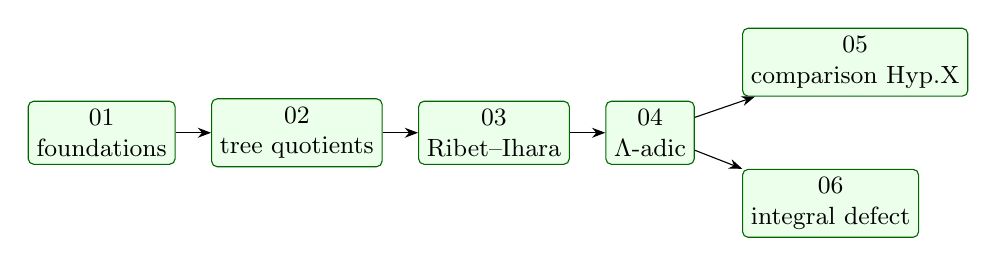
\begin{tikzpicture}[node distance=0.5cm and 0.45cm, >={Stealth},
  st/.style={draw,rounded corners=2pt,inner sep=3pt,font=\small,align=center,fill=green!8,draw=green!40!black}]
  \node[st] (s1) {01\\foundations};
  \node[st,right=of s1] (s2) {02\\tree quotients};
  \node[st,right=of s2] (s3) {03\\Ribet--Ihara};
  \node[st,right=of s3] (s4) {04\\$\Lambda$-adic};
  \node[st,above right=0.05cm and 0.6cm of s4] (s5) {05\\comparison $\HypX$};
  \node[st,below right=0.05cm and 0.6cm of s4] (s6) {06\\integral defect};
  \draw[->] (s1)--(s2); \draw[->] (s2)--(s3); \draw[->] (s3)--(s4); \draw[->] (s4)--(s5); \draw[->] (s4)--(s6);
\end{tikzpicture}\\[2pt]
{\small All six stages are closed and merged (milestone closures S01--S06, 14--15 November 2026).}
\end{center}

\subsection{HACS}
HACS (\emph{Harder Arithmetic Cohomology System}; Fabian Januszewski) computes the cohomology of arithmetic groups with
integral coefficients, the Hecke action and congruence phenomena, via simplicial orbifold models (C++/AVX-512/CUDA). It is released as v0.2.1 \cite{HACS021} with census data hacs-data v0.2.0 \cite{HACSdata020}; the snapshot
in \texttt{code/hacs/} is HACS v0.2.1 plus our clearly marked JL module, three documented hook lines (a \texttt{CMakeLists.txt}
include and the \texttt{RegisterJL} declaration and call) and the regenerated CLI manual tables (\texttt{code/hacs/CHANGES.md}). In this project HACS was used in two lanes (\S\ref{ss:hacs}): Lane~A
bridges our Python/PARI results to HACS (definite local algebras, the Betti side of T4, a Brandt-lattice export format),
and Lane~B adds a native quaternion core and exact integral congruence modules of Brandt lattices read through HACS's
integral engine. Every HACS number in this report is \emph{computed}; nothing is called ``certified''.

\subsection{The agentic process}
The work was carried out by a hierarchy of Claude Code agents coordinated through git: a global master on Fabian's node
delegates to stage masters and work-package agents (Haiku, Sonnet, Opus; Fable for audits), two further machines (TITAN,
CONCEPTD) run all Lean builds and the from-scratch final gates, and Abhijit's node (a separate account) takes work
packages over a git message channel, including cross-account blind reviews. Each stage ran through a staged plan, work
packages on branches, batched integration builds, an early gate, parallel Fable Lean and chapter audits, and a
from-scratch final gate on two machines. Stage wall times were about $2.2$, $1.3$, $1.1$, $2.2$, $1.1$ and $1.2$ hours
(stages 01--06). Decisions of mathematical substance (e.g.\ FD1, FD2 and the case $q\equiv-1\bmod p$, \S\ref{sec:open}) were
taken by Fabian. The process is documented in \texttt{docs/agentic-process/}.

\subsection{Status legend}\label{ss:legend}
Statuses are those of the chapters, never upgraded. The markers are the macros of \texttt{mathematics/preamble.tex}:
\begin{center}\small
\begin{tabular}{@{}l p{0.68\textwidth}@{}}\toprule
marker & meaning\\\midrule
\stproved & proof written in the chapter\\
\stpmc & proved here, modulo the cited inputs named in the statement\\
\stcited & taken from the literature, with a precise pointer\\
\stknown & standard / textbook, reference given\\
\stformal{} / \stformalized & exists in Lean 4 (declaration names given by \lean{\dots}); \emph{formalized modulo $H$}: the Lean statement takes the registered hypotheses $H$ as explicit arguments\\
\stcomp & machine computation, result file under \texttt{code/results/}\\
\stconj{} / \stexp & conjectural / expected\\
\stopen & open (no proof claimed)\\
\stsketch & sketched (argument not complete)\\
\sttoprove & still to be proved (planning marker)\\
\sthyp & a hypothesis, assumed\\
\leanplanned & formalization planned, not done at that point\\
\provisional{\dots} & a change made provisionally after the global seam audit, pending Fabian's review\\\bottomrule
\end{tabular}
\end{center}
A Lean \emph{hypothesis} \texttt{Hyp.X} is a named \texttt{Prop} taken as an explicit argument, never an \texttt{axiom}.
A toy instance of a hypothesis in the Lean tests shows consistency (non-vacuity) only and is never called evidence.

% SPDX-License-Identifier: CC-BY-4.0
% Copyright (C) 2026 Fabian Januszewski, Abhijit (the Langlandscape team)
\section{Results of the six stages}\label{sec:results}

\paragraph{How this section is made.} Each box below is a statement copied \emph{verbatim} from the chapter source
\texttt{mathematics/chapters/s0N/*.tex} by \texttt{tools/extract\_statements.py}, including its status markers and
\verb|\provisional| notes. Where the chapter prints the status in a paragraph directly after the statement (as in stage~02
and in parts of stage~04), that paragraph is copied as well, below the statement and marked as such; a \stformal{} there
is the Lean status of the result (for Thm~6.1 and Thm~6.3 a schematic interface), not a claim about its mathematics. The only changes are mechanical: the \verb|\label| is moved into the box header, and every
cross-reference is replaced by its number in \mainpdf{} (built from the chapters of this submission tree, 170 pp; Lean tree 2323a252); so ``Thm~21.5'' inside a box
means Theorem~21.5 of \mainpdf. Hypotheses such as (H0)--(H2), (P), (Lev) and the cited inputs are defined there.
Each header gives the number and page in \mainpdf{} (the page is that of the label; in a few cases the statement
starts on the next page). Proofs are not reproduced. A box may carry several status markers;
each marker refers to the part of the statement it is attached to. Table~\ref{tab:allresults} at the end of the section
lists every theorem, proposition, corollary and conjecture of the chapters with the markers occurring in its statement.

\subsection{Stage 01: quaternionic foundations}
Chapter: \mainpdf, pp.~1--24. Lean: 17 results of the chapter are marked formalized (milestone closure S01).
% SPDX-License-Identifier: CC-BY-4.0
% Copyright (C) 2026 Fabian Januszewski, Abhijit (the Langlandscape team)
% GENERATED by tools/extract_statements.py from mathematics/chapters/ -- do not edit by hand.

\begin{quoted}{Theorem}{2.1}{31}{thm:s01-mass}{Eichler mass formula; \texttt{if:s01-mass}}{chapters/s01/2-mass.tex}
\begin{enumerate}[label=(\alph*)]
\item $\displaystyle\sum_{[x]\in\XB{\hat\cO^\times}}\frac1{|\Gamma_x|}=\frac{1}{24}\prod_{\ell\mid D}(\ell-1)$
  (full-unit convention), equivalently $\sum 1/w_x=\varphi(D)/12$.
\item (level change) For open $U'\le U\le\hat\cO^\times$: $\sum_{X_B(U')}1/|\Gamma_{x'}(U')|=[U:U']\sum_{X_B(U)}1/|\Gamma_x(U)|$.
  With $w$ in place of $|\Gamma|$ the same holds iff $-1\in U'$ or $-1\notin U$; if $-1\in U\setminus U'$ then
  $2\sum_{X_B(U')}1/w_{x'}=[U:U']\sum_{X_B(U)}1/w_x$ (\lean{Langlandscape.Quat.massW\_level\_change\_two}).
\item $[\hat\cO^\times:\Uzero{N}]=\psi(N)=N\prod_{\ell\mid N}(1+\ell^{-1})$ and $[\hat\cO^\times:\Uone{N}]=\psi(N)\varphi(N)=N^2\prod_{\ell\mid N}(1-\ell^{-2})$.
\item Hence $\sum_{\XB{\Uzero{N}}}1/w_x=\varphi(D)\psi(N)/12$, and for $p\ge5$, $p\nmid D$, $s\ge1$, $(M,pD)=1$:
\[|S_s|=|\XB{\Uone{Mp^s}}|=\frac{\varphi(D)}{24}\,\psi(Mp^s)\,\varphi(Mp^s).\]
\end{enumerate}
Status: (a) \stcited{} \lit{voight\_2021\_quaternion-algebras}{Thm.~25.1.1, p.~415 (with $w_J=\#\cO_L(J)^\times/\{\pm1\}$,
hence $1/12$)}; \lit{eichler\_1955\_zur-zahlentheorie-der-quaternionen-algebren}{\S4 ``Klassenzahl und Maß'', p.~136ff.};
in Lean it is the registered hypothesis \pathtt{Hyp.EichlerMass} (\Tpath{Hyp/EichlerMass.lean}, $1/24$, full units), proved
for $D=2,11$ in tests. (b) \stformal{} \Tpath{P2/Mass.lean} \pathtt{mass\_orbit\_count}; the $w$-variant \stformal{} \pathtt{Quat.massW\_level\_change},
\pathtt{Quat.massW\_level\_change\_two} (orbit counting). (c) first half \stformal{} \pathtt{gl2\_borel\_index}, \pathtt{mass\_level\_change}; second half
\stproved{} below (count $|\GL_2(\Z/N)|/(N\varphi(N))$). (d) first half \stpmc{} from (a)--(c) (proof below; cf.\ \lit{voight\_2021\_quaternion-algebras}{Thm.~25.3.18,
p.~423}), \stpmc{} in Lean as \pathtt{eichlerOrder\_mass} (under \pathtt{Hyp.EichlerMass}); second half \stpmc{} from (a)--(c)
and Lemma~1.7(b) (all $\Gamma_x=1$), and \stformal{} under \pathtt{Hyp.EichlerMass} as \pathtt{Quat.card\_XB\_Utower}.
\end{quoted}

\begin{quoted}{Theorem}{6.1}{48}{thm:s01-JLclassical}{classical JL, Brandt form; \pathtt{if:s01-targets}; seed Thm.~3.1}{chapters/s01/6-targets.tex}
Let $(M,D)=1$; for the $\Gamma_0$ statement let $k\ge2$ be even. Choosing $\Qp\hookrightarrow\C$ (or working with the import's global splitting over a number
field), there is an isomorphism of modules over the algebra generated by the $T_\ell$, $\ell\nmid DM$,
\[\Brandt{\Uzero{M}}{V_k}\otimes\C\ \cong\ S_k(\Gamma_0(DM))^{D\text{-new}}\ \oplus\ \begin{cases}\C\cdot\mathbf 1&k=2,\\0&k>2,\end{cases}\]
where $\mathbf 1$ spans the functions factoring through $\Nrd$ (one-dimensional since $\Q_{>0}\backslash\hat\Q^\times/\Zhat^\times=1$),
and $H^1_{\rm par}(\Gamma_0(DM),V_k\otimes\C)\cong S_k\oplus\overline{S_k}$. At $\Gamma_1$-level, for $(N,D)=1$ and $k\ge2$ of any parity: for $k\ge3$,
$\Brandt{\Uone{N}}{V_k}\otimes\C\cong S_k(\Gamma_1(N)\cap\Gamma_0(D))^{D\text{-new}}$, and for $k=2$ the same after dividing
by the functions factoring through $\Nrd$, compatibly with $T_\ell,S_\ell$ for $\ell\nmid ND$.
\stcited{} \lit{jacquet-langlands\_1970\_automorphic-forms-on-gl2}{Thm.~16.1 (LNM~114, p.~494; p.~250 in the retypeset copy in \pathtt{literature/}) (representation-theoretic; JL call
their proof a sketch)}; \lit{buzzard\_2004\_p-adic-families-of-automorphic-forms\_preprint}{Thm.~2, p.~13 ($\Gamma_1$ form,
attributed to JL, Shimizu, Arthur)}; \lit{hijikata-pizer-shemanske\_1980\_basis-problem-for-modular-forms-announcement}{\S0,
p.~280 (basis problem, all $N$)}; \lit{shimizu\_1965\_zeta-functions-of-quaternion-algebras}{(scan; not text-verified)};
\lit{pizer\_1980\_an-algorithm-for-computing-modular-forms-on-gamma0-n\_scan}{(scan; not text-verified; algorithmic side)};
survey \lit{voight\_2021\_quaternion-algebras}{Remark~41.5.13, p.~778 (historical account of the correspondence; the
statement itself is not formulated there)}.
\par\smallskip\noindent{\scriptsize\itshape [Status paragraph following the statement in the chapter:]}\par
\noindent\emph{Lean status.} \lean{Langlandscape.Hyp.JLClassical} \stformal{} as a \emph{schematic interface} (S01-L13): only the case $k=2$
with trivial coefficients, the Eisenstein line $\C$ with $T_\ell=\ell+1$, and an abstract Hecke module in place of
$S_k(\Gamma_0(DM))^{D\text{-new}}$. It is a statement about the true space only once that space is substituted for the abstract datum, which cannot be checked
in Lean here; no later result may be advertised as ``under classical JL'' without this caveat.
\end{quoted}

\begin{quoted}{Theorem}{6.3}{49}{thm:s01-lambdaJL}{$\Lambda$-adic Hecke JL}{chapters/s01/6-targets.tex}
Let $\T^{\ord}(DM)$ be Hida's ordinary $\Lambda$-adic Hecke algebra of tame level $\Gamma_1(M)\cap\Gamma_0(D)$ and
$\T^{\ord}_B(M)$ the one acting on $\varprojlim_se\,\Brandt{U_s}{\cOE}$ (or on its homological dual). There is a surjection
$\T^{\ord}(DM)\twoheadrightarrow\T^{\ord}_B(M)$ with $T_\ell\mapsto T_\ell$ ($\ell\nmid DMp$), $U_\ell\mapsto U_\ell$ ($\ell\mid Mp$),
classical $\langle d\rangle\mapsto$ seed $\langle d\rangle^{-1}$ for $d$ prime to $Mp$ (the guard $\gcd(d,Mp)=1$, stated in \lean{Langlandscape.Hyp.LambdaJL} as \texttt{Nat.Coprime d (M*p)}, S04-L17a; the diamonds are defined only for such $d$; the seed's adelic diamond, right translation by $\mathrm{diag}(1,d)$; Remark~4.5, Lemma~5.5), and $U_\ell\mapsto+\Pi_\ell$ ($\ell\mid D$), $\Pi_\ell$ acting by right translation; Hsieh writes $-$, which is not imported (stage 05, \pathtt{rem:s05-hsieh}),
\provisional{F6/D3: sign fixed to $+\Pi_\ell$, Hsieh's sign declared not imported; before: $U_\ell\mapsto\pm\Pi_\ell$ ($\ell\mid D$; sign convention-dependent); the Hsieh citation below read ``$\mathrm{JL}(U_q)=-U_q$ for $q\mid N^-$'' without the remark that it is not imported.}
whose kernel cuts out the
$D$-new quotient: $\T^{\ord,D\text{-new}}\cong\T^{\ord}_B$.
\stcited{} \lit{longo-vigni\_2009\_quaternion-algebras-heegner-points-and-the-arithmetic-of-hida-families\_arxiv}{Prop.~6.1,
p.~27 (iso of $\tilde\Lambda$-algebras $\T^{\ord}_\infty\simeq\mathbb B^{\ord}_\infty$, with $T(n,n)=\langle n\rangle$ normalised as in
their [25])}; \lit{hsieh\_2017\_hida-families-and-p-adic-triple-product-l-functions\_arxiv}{\S4.5, p.~34 (surjection
$\mathrm{JL}:\T(N,\mathbb I)\to\T^D(N,\mathbb I)$, with his sign $\mathrm{JL}(U_q)=-U_q$ for $q\mid N^-$, not imported)}.
\par\smallskip\noindent{\scriptsize\itshape [Status paragraph following the statement in the chapter:]}\par
\noindent\emph{Lean status.} \lean{Langlandscape.Hyp.LambdaJL} \stformal{} as a \emph{schematic interface} (S01-L13): two conjuncts, the surjection
$\varphi$ with the generator matching (including classical $\langle d\rangle\mapsto$ seed $\langle d\rangle^{-1}$ and $U_\ell\mapsto+\Pi_\ell$ for $\ell\mid D$; the diamond field of the Lean hypothesis is corrected to the inverse diamond on the Lean side, S04) and $\ker\varphi=$ an abstract ideal cutting out the $D$-new
quotient. The $\GL_2$ side (algebra, generators, ideal) is abstract data, so the hypothesis is $\Lambda$-adic JL only after instantiation by the true objects.
\end{quoted}


\subsection{Stage 02: tree quotients}
Chapter: \mainpdf, pp.~24--50. 72 \verb|\lean| markers at the S02 closure.
% SPDX-License-Identifier: CC-BY-4.0
% Copyright (C) 2026 Fabian Januszewski, Abhijit (the Langlandscape team)
% GENERATED by tools/extract_statements.py from mathematics/chapters/ -- do not edit by hand.

\begin{quoted}{Theorem}{7.7}{54}{thm:s02-SA}{strong approximation for $B^1$ at $S=\{\infty,q\}$}{chapters/s02/2-quotient.tex}
Since $q\nmid D$, $B_q\cong M_2(\Qq)$ is split and $B^1_q\cong\SL_2(\Qq)$ is non-compact. Hence $B^1$ (embedded diagonally) is
dense in the restricted product $\Bhat^{1,(q)}:=\prod'_{\ell\ne q}B^1_\ell$ (with respect to the $\cO^1_\ell$).
\smallskip

\noindent\emph{Consequence (the shape used; \texttt{if:s02-SA}).} For every $q$-admissible $U$,
\[\Bhat^1=B^1\big(B^1_q\times U^{1,(q)}\big).\tag{SA$_U$}\]
\par\smallskip\noindent{\scriptsize\itshape [Status paragraph following the statement in the chapter:]}\par
\noindent\emph{Status.} The theorem is \stcited{}:
\lit{voight\_2021\_quaternion-algebras}{Main Thm.~28.5.3, p.~485}, applied to the global ring $R=\Z[1/q]$ with eligible set
$S=\{\infty,q\}$. In Voight's notation $\Bhat=\Bhat^S=\prod'_{v\notin S}B_v$ is the $S$-finite adele ring
(\lit{voight\_2021\_quaternion-algebras}{27.6.4, p.~469}; there, when $S$ is clear from the context, the superscript $S$ is dropped and replaced by hats), so his
$\Bhat^1$ is our $\Bhat^{1,(q)}$. The hypothesis ``$B$ is $S$-indefinite'' (\lit{voight\_2021\_quaternion-algebras}{Def.~28.5.1,
p.~485}: $S$ contains a place unramified in $B$) holds because $q\in S$ and $q\nmid D$.
Equivalently \lit{vigneras\_1980\_arithmetique-des-algebres-de-quaternions}{Ch.~III, Thm.~4.3, p.~81} ($H^1_KH^1_S$ dense in
$H^1_{\A}$ if $H^1_S$ is not compact; page-checked) and
\lit{platonov-rapinchuk\_1994\_algebraic-groups-and-number-theory\_2up}{\S7.4, Thm.~7.12, p.~427} (page-checked in the M8 litnote).
Kneser \lit{kneser\_1969\_lectures-on-galois-cohomology-of-classical-groups}{\S5.5, Sublemma~b, p.~94 (Tata pagination; p.~72 of the scan)} only states the result;
it is listed for orientation and not relied upon. The consequence (SA$_U$) is \stproved{} below from the theorem. It is
\lit{voight\_2021\_quaternion-algebras}{28.4.8, p.~484} (density implies $\Bhat^1\subseteq B^1\hat\cO^1$) and
\lit{voight\_2021\_quaternion-algebras}{Cor.~28.5.12, p.~486}; the shape (SA$_U$), with the factor $B^1_q$, is the projection away from $\infty$ of the \emph{second}
equality of (28.5.13) there (which multiplies in $B^1_S=B^1_\infty\times B^1_q$). Both are stated only for the norm-one units $\hat\cO^1$ of an
$R$-order $\cO$, not for a general open subgroup; the same proof extends, since it uses only that $\hat\cO^1$ is open (proof below); this matters because $U^{(q)}$ need not be the unit group of an order (e.g.\ $\Uone{N}$-levels).
In Lean, (SA$_U$) for all admissible $U$ is registered as the hypothesis $\HypSA$, \lean{Langlandscape.Hyp.SA} (shape
\lean{Langlandscape.Tree.SAat}, quantified over \pathtt{Tree.IsQAdmissible}); this is a registered hypothesis, not a proof, and the
theorem stays \stcited. The derivation of (SA$_U$) from density below is not formalised. Per level, $\HypSA$ is replaced by
Prop.~7.9.
\end{quoted}

\begin{quoted}{Proposition}{7.9}{55}{prop:s02-BG}{SA for one level as a finite check}{chapters/s02/2-quotient.tex}
Let $U$ be $q$-admissible. The maps
\begin{gather*}
\phi_0:\GU\backslash V_0(\cT_q)\to\XB U,\ \GU gv_0\mapsto[g];\\
\phi_1:\GU\backslash V_1(\cT_q)\to\XB U,\ \GU g\alpha v_0\mapsto[g\alpha];\\
\phi_E:\GU\backslash E(\cT_q)\to\XB{U'},\ \GU ge_0\mapsto[g]
\end{gather*}
($g\in B^1_q$) are well defined and \emph{injective}, and $\phi=(\phi_0,\phi_1,\phi_E):\GU\backslash\cT_q\to\BG(U,q)$ is a locally
surjective morphism of graphs. The following are equivalent:
\begin{enumerate}[label=(\roman*)]
\item $\phi_0$ is surjective;
\item (SA$_U$) holds and $\Xone(U)\to\XB{U}$ is surjective;
\item $\BG(U,q)$ is connected.
\end{enumerate}
Moreover:
\begin{enumerate}[label=(\alph*)]
\item (i) implies that $\phi_0,\phi_1,\phi_E$ are all bijective, so $\phi$ is an isomorphism of graphs $\GU\backslash\cT_q\cong\BG(U,q)$.
  This implication does not use the connectedness of $\cT_q$.
\item In all cases, $\phi$ is an isomorphism of $\GU\backslash\cT_q$ onto a union of connected components of $\BG(U,q)$ containing
  $([1],0)$; using that $\cT_q$ is connected, onto the connected component of $([1],0)$.
\end{enumerate}
\par\smallskip\noindent{\scriptsize\itshape [Status paragraph following the statement in the chapter:]}\par
\noindent\emph{Status.} \stproved{} (new in this plan). No strong approximation is used. The connectedness of $\cT_q$
(Lemma~7.3(a), \stcited) enters only in (i)$\Rightarrow$(iii) and in the last clause of (b); the implications
(iii)$\Rightarrow$(i)$\Leftrightarrow$(ii), the injectivity, local surjectivity, and (a) are tree-free.
In particular Thm.~7.7 together with Hasse--Schilling (Lemma~7.6(b)) implies (ii), hence (i) and the
bijections of (a) (tree-free), and hence (iii) (using connectedness of $\cT_q$). As hypotheses, SA alone does not give (ii).
Conversely, for an explicit $(B,U,q)$ the condition (iii) is a finite computation, and it discharges (SA$_U$) and the surjectivity
of $\Xone(U)\to\XB U$ for that level. Classically, SA enters at this point through the definite analogue of Ihara's lemma:
\lit{diamond-taylor\_1994\_non-optimal-levels-of-mod-l-modular-representations}{Lemma~2 and Cor.~1, pp.~445--446} show that $T_\ell-2$, $S_\ell-1$ annihilate $A[l]$, $A$ the kernel of
$(f_1,f_2)\mapsto f_1+\varphi_pf_2$ on $S_k(U;\Q_l/\Z_l)^2$, for almost all $\ell\equiv1\bmod d$ (Lemma~2; hypotheses $p\nmid N_U l$), whence the Eisenstein statement (Cor.~1), and the paper says this lemma ``plays the role of Ihara's result'' (p.~445).
\emph{Lean status.} \stformal{} (all tree-free parts; in the coset model of Lemma~7.3, with $\phi_0,\phi_1$ combined
into one map \texttt{phiV} on all vertex orbits to $\XB U\sqcup\XB U$):
\lean{Langlandscape.Tree.phiV\_injective}, \lean{Langlandscape.Tree.phiE\_injective},
\lean{Langlandscape.Tree.phiV\_oO}, \lean{Langlandscape.Tree.phiV\_tO} (Step~3),
\lean{Langlandscape.Tree.phi\_locSurj\_type0}, \lean{Langlandscape.Tree.phi\_locSurj\_type1} (Step~4);
(i) is \lean{Langlandscape.Tree.surjType0} (every class of $\XB U$ is $[g]$ with $g\in\SL_2(\Qq)$), and
\lean{Langlandscape.Tree.surjType0\_iff} identifies it with the surjectivity of $\phi_0$;
\lean{Langlandscape.Tree.surjType0\_of\_BGConnected} ((iii)$\Rightarrow$(i)),
\lean{Langlandscape.Tree.bijective\_of\_BGConnected} ((iii)$\Rightarrow$ bijections),
\lean{Langlandscape.Tree.bijective\_of\_surjType0} ((a)), \lean{Langlandscape.Tree.surj\_of\_SA} ((ii)$\Rightarrow$(i)),
\lean{Langlandscape.Tree.SA\_of\_surj} ((i)$\Rightarrow$(ii)). None of these takes a \texttt{Hyp.*} argument.
(i)$\Rightarrow$(iii) is \lean{Langlandscape.Tree.BGConnected\_of\_surj}, formalized modulo \texttt{Hyp.BTtree}; the ``in particular''
is \lean{Langlandscape.Tree.BGConnected\_of\_SA\_HS}, formalized modulo $\HypSA$, $\HypHS$, \texttt{Hyp.BTtree} (and
\lean{Langlandscape.Tree.surjType0\_of\_SA\_HS} for (i), modulo $\HypSA$, $\HypHS$ only). The last clause of (b) (image $=$ the
component of $([1],0)$) also uses connectedness of $\cT_q$; it has no separate Lean declaration (not formalised; it would take
\texttt{Hyp.BTtree}).
\emph{Hypothesis on $U$ in Lean} (audit note): all of these except \pathtt{BGConnected\_of\_SA\_HS} and \pathtt{surjType0\_of\_SA\_HS}
assume only that $U$ is a $q$-level (\texttt{IsQLevel}: $U\le\hat\cO^\times$ of finite index, factoring at $q$), not that $U$ is
$q$-admissible; the condition $\Nrd U=\Zhat^\times$ is not needed for the proposition, in line with the proof above (Step~2 uses only
$\Nrd U\subseteq\Zhat^\times$).
\emph{Deviation from the plan tex (refinement).} The tex's ``Moreover, in all cases the maps are injective and $\phi$ is an isomorphism
onto the component of $(1,0)$'' is split here into the injectivity/local surjectivity in the statement, (a) ((i)$\Rightarrow$ bijections,
tree-free) and (b) (union of components, tree-free; single component, with the tree).
\end{quoted}

\begin{quoted}{Proposition}{7.10}{57}{prop:s02-quot}{quotient graph; seed Prop.~quot}{chapters/s02/2-quotient.tex}
Let $U$ be $q$-admissible and assume (iii) of Prop.~7.9. By Prop.~7.9 this holds given
Thm.~7.7, Hasse--Schilling \emph{and} the connectedness of $\cT_q$ (Lemma~7.3(a), \stcited; \textbf{[tree]}):
$\HypSA\wedge\HypHS\wedge\mathrm{Hyp.BTtree}\Rightarrow$ (iii) (Lean \pathtt{Tree.BGConnected\_of\_SA\_HS}, which takes \texttt{Hyp.BTtree});
the bijections of (a) need only $\HypSA\wedge\HypHS$. As hypotheses, SA alone does not suffice.
(iii) itself is the working hypothesis here.
\begin{enumerate}[label=(\alph*)]
\item There are bijections
  \begin{gather*}
    \GU\backslash\{\text{type-}0\text{ vertices}\}\ \xrightarrow{\ gv_0\mapsto[g]\ }\ \XB{U},\\
    \GU\backslash\{\text{type-}1\text{ vertices}\}\ \xrightarrow{\ g\alpha v_0\mapsto[g\alpha]\ }\ \XB{U},\\
    \GU\backslash\{\text{edges}\}\ \xrightarrow{\ ge_0\mapsto[g]\ }\ \XB{\Uzero{q}U}
  \end{gather*}
  ($g\in B^1_q$). Under these bijections the endpoint maps $o,t$ become $s_0,s_1$. In other words,
  $\GU\backslash\cT_q\cong\BG(U,q)$ as graphs.
\item For $g\in B^1_q$, $\Stab_{\GU}(gv_0)=\Gamma_g$ (level $U$), $\Stab_{\GU}(g\alpha v_0)=\Gamma_{g\alpha}$
  (level $U$) and $\Stab_{\GU}(ge_0)=\Gamma_g$ (level $\Uzero{q}U$). For another representative
  $x'=\gamma xu$ one has $\Gamma_{x'}=\gamma\Gamma_x\gamma^{-1}$. Each $\Gamma_x$ has norm $1$
  (Lemma~1.7(a)), so it lies in $\GU$ after conjugation.
\item Let $T$ be any Hecke operator supported away from $q$ ($T_\ell,S_\ell,U_\ell$ for $\ell\mid M$,
  $\langle d\rangle$, $U_p$ with the normalisation $\NUp$ of stage 01, and $\Pi_\ell$ for $\ell\mid D$),
  acting compatibly on levels $U$ and $\Uzero{q}U$. Then $s_0^*,s_1^*,s_{0*},s_{1*}$ commute with $T$ on
  Brandt modules $\Brandt{\cdot}{V}$ and on their homological versions (on $\Brandt{\cdot}{V}$, $s_{j*}$ means the trace
  $\mathrm{tr}_j$ of Def.~7.13).
\end{enumerate}
\par\smallskip\noindent{\scriptsize\itshape [Status paragraph following the statement in the chapter:]}\par
\noindent\emph{Status.} (a): \stproved{} given (iii); \stpmc{} via Thm.~7.7 and Hasse--Schilling (through
(ii)$\Rightarrow$(i)$\Rightarrow$(a), which does not use connectedness of the tree). (b): \stproved; \emph{refinement of the plan tex} (which has ``given (iii)''): the three stabiliser identities
hold for every $g\in B^1_q$ without (iii); (iii) is used only to know that every class of $\XB U$, $\XB{U'}$ has such a tree
representative. (c): \stproved{} (unconditional).
\end{quoted}

\begin{quoted}{Proposition}{7.19}{66}{prop:s02-harm}{harmonic cochains; seed Prop.~harm}{chapters/s02/3-cohomology.tex}
Under the hypotheses of Prop.~7.18(b), let $c$ be a function on oriented edges with values in $V$
such that $c(\gamma e)=\gamma_p\,c(e)$ for $\gamma\in\GU$, $c(\bar e)=-c(e)$, and $\sum_{o(e)=v}c(e)=0$ for all
$v$. The $\GU$-invariant $V$-valued harmonic cochains of this kind are
\[\ker\Big(\Brandt{\Uzero{q}U}{V}\xrightarrow{(\mathrm{tr}_0,\,\mathrm{tr}_1)}\Brandt{U}{V}^{2}\Big)\ \cong\ H_1(\GU,V),\]
with the trace maps $\mathrm{tr}_j$ (the plan's ``$s_{j*}$'') of Def.~7.13. If $-1\in U$, assume $-1$ acts trivially on $V$
(the standing hypothesis of Def.~7.13, needed for $\nu$); otherwise replace $V$ by $V^+$, as $V^-$ contributes $0$ to both sides
(Remark~7.15). This is the \emph{$q$-new} submodule of the Brandt
module of level $\Uzero{q}U$; the term is defined here as this kernel. The isomorphism is $\nu_{U'}^{-1}$ followed by
Prop.~7.18(b), $H_1(\GU,V)=\ker\partial$.
\par\smallskip\noindent{\scriptsize\itshape [Status paragraph following the statement in the chapter:]}\par
\noindent The description of the harmonic cochains as $\ker(\mathrm{tr}_0,\mathrm{tr}_1)$ is \stproved{} given (iii); the isomorphism with
$H_1(\GU,V)$ is \stpmc{} given (iii) (via Prop.~7.18(b); registered in Lean as hypothesis \pathtt{Hyp.SerreCoh}). (In
the sum, ``$o(e)=v$'' runs over all oriented edges with origin $v$, in both orientation classes.)
\emph{Lean status.} For trivial coefficients $V=R$ the $q$-new module $\ker(\mathrm{tr}_0,\mathrm{tr}_1)$ is
\lean{Langlandscape.Tree.qNew}, and $\nu_{U'}:\ker\partial\cong\ker(\mathrm{tr}_0,\mathrm{tr}_1)$ is \stformal{}
\lean{Langlandscape.Tree.qNewEquivKerPartial} (also \lean{Langlandscape.Tree.normMap\_restrict\_bijective}), assuming all $w_x$
at level $U$ are units in $R$ (remark below); no (iii) is needed for it. The identification with harmonic cochains on the tree is not
formalised.
\end{quoted}


\subsection{Stage 03: weighted graphs, the definite Ribet sequence and the Ihara lemma}
Chapter: \mainpdf, pp.~50--82.
% SPDX-License-Identifier: CC-BY-4.0
% Copyright (C) 2026 Fabian Januszewski, Abhijit (the Langlandscape team)
% GENERATED by tools/extract_statements.py from mathematics/chapters/ -- do not edit by hand.

\begin{quoted}{Proposition}{8.8}{79}{prop:s03-mazur}{Mazur check; seed Example mazur}{chapters/s03/1-graphs.tex}
For every prime $q$,
\[\Phicomb\big(\GDR_q(\hat\cO^\times)\big)\ \cong\ \Z\big/\mathrm{num}\tfrac{q-1}{12},\]
and this group is cyclic, generated via $\bar\lambda$ of Lemma~8.4. For $q\in\{2,3\}$ both sides are trivial.
\stpmc: Lemma~8.7, Prop.~8.3, Lemma~8.4. Lean (S03-L5, L6):
\lean{Langlandscape.Graph.mazurNum}, \lean{Langlandscape.Graph.mazur\_prod\_mul\_sum}, \lean{Langlandscape.Graph.mazur\_weights\_pairwise\_coprime}
\stformal{} (abstract arithmetic core: for weights in $\{1,2,3\}$ with the counts $n_2,n_3$ and $\sum w^{-1}=\frac{q-1}{12}$ one has
$\prod w\cdot\sum w^{-1}=\mathrm{num}\frac{q-1}{12}$, and the weights are pairwise coprime; $q\ge5$ only); the identification of the weights with the DR graph
(\lean{Langlandscape.Ribet.sum\_inv\_wx\_Ohat}, \lean{Langlandscape.Ribet.mazur\_check}, \stformal{} modulo the registered hypothesis \lean{Langlandscape.Hyp.EllipticCount} (and \pathtt{Hyp.EichlerMass})); the cases $q=2,3$ are \stformal{} as well, through the $q\le3$ clause of the same hypothesis \lean{Langlandscape.Hyp.EllipticCount} (which asserts $|\XB{\hat\cO^\times}|=1$ there; \lean{Langlandscape.Ribet.mazur\_check} covers every prime $q$), so the chapter's elementary derivation of that case is not formalized
\end{quoted}

\begin{quoted}{Proposition}{9.5}{83}{prop:s03-phieis}{$\Phicomb$ is Eisenstein}{chapters/s03/2-eisenstein.tex}
Let $q$ be any prime, $U=\Uzero M$, $B=B_q$, $\ell\nmid qM$, and let $T_\ell$ act on $\Z[\XBq U]$ by the Brandt matrix (homological
convention, $[x]\mapsto\sum_i[xg_i]$). Then $T_\ell$ is self-adjoint for $\langle,\rangle_w$, so it acts on $\Phicomb(\GDR_q(U))$, and
$T_\ell-(1+\ell)$ annihilates $\Phicomb(\GDR_q(U))$. \stproved{} (proof below, steps (1)--(4); valid for all primes $q$, including $q\in\{2,3\}$, and all
$M$ with $q\nmid M$ and $\ell\nmid qM$; it uses Lemma~9.2, Prop.~3.3(a),(b), Prop.~8.3, and the
finiteness of $\XBq U$, Prop.~1.6, which makes $\GDR_q(U)$ a finite graph). Lean: abstract core \stformal{}: \lean{Langlandscape.Graph.heckeQ} and \lean{Langlandscape.Graph.phiComb\_eisenstein} (steps (2)--(4), abstract: an integer matrix $B$ with row sums $\ell+1$,
$w_{e'}B(e,e')=w_eB(e',e)$ and $w_e\mid B(e,e')$ off the diagonal, acting on $\Phicomb$ of the two-vertex lattice $\Z[E]^0$ with weights $w_e>0$). Instantiation at $U=\hat\cO^\times$: \lean{Langlandscape.Ribet.phiComb\_eisenstein\_Ohat} \stformal{} modulo the registered hypothesis (step (1)) \lean{Langlandscape.Hyp.BrandtStabFree}.

Cross-references (not needed for the proof): [Ri90, Thm~3.12, p.~449; proof pp.~449--450, Remark~3.13] \stcited{}
\lit{ribet\_1990\_modular-representations-of-gal-qbar-q-arising-from-modular-forms}{Thm 3.12, p.~449}. Ribet's $\Phi=\coker(\iota)$ is our
$\Phicomb$, and his proof is the divisibility of the off-diagonal Brandt entries $B_\ell(i,j)$ by $e(i)=w_i$, which is step~(1) below, a purely quaternionic
fact. The geometric analogue for $\Phi_{N,p}$ is [Ed91, Th.~1, p.~163] \stcited{}
\lit{asterisque\_1991\_courbes-modulaires-et-courbes-de-shimura\_vol}{Edixhoven, Th\'eor\`eme~1, p.~163}, which assumes $p>3$.
\end{quoted}

\begin{quoted}{Theorem}{10.2}{89}{thm:s03-ribet}{definite Ribet sequence as a vertex collapse; seed Thm ribet}{chapters/s03/3-ribet.tex}
Let $q\nmid D$, $U$ as in \texttt{if:s02-quot}, $\G:=\GU\quot\cT_q$, and $|\G|$ its underlying graph, with the orientation (C1).
\begin{enumerate}[label=(\alph*)]
\item Over $\Z$ there is an exact sequence, equivariant for all Hecke operators $T=[UgU]$ with $g$ supported at a finite set $\Sigma\not\ni q$ of
  places at which $U$ is factorisable (Prop.~7.10(c); this holds for all standard levels):
  \[0\to H_1(|\G|,\Z)\to\Z[\XB{U'}]^0\xrightarrow{\ \alpha=(-s_{0*},\,s_{1*})\ }\big(\Z[\XB U]^0\big)^{2}\to0.\]
\item Let $p\ge5$ and let $V$ be a finitely generated $\Zp$-module with continuous $U_p$-action. Then, with the traces of (C3),
  \[0\to H_1(\GU,V)\to\Brandt{U'}V\xrightarrow{\alpha}\Brandt UV^{2}\to H_0(\GU,V)\to0.\]
\item $\rk_\Z H_1(|\G|)=|\XB{U'}|-2|\XB U|+1$. At a level where all $\Gamma_x$ are trivial, this is $(q-1)|\XB U|+1$, as in
  \pathtt{if:s02-indef}. For $V=\Zp$, $p\ge5$: $H_1(\GU,\Zp)=H_1(|\G|,\Z)\otimes\Zp$.
\end{enumerate}
Part (a) holds over every commutative ring $R$ in place of $\Z$ (with $H_1(|\G|,R)$).
\emph{Status.} Given (iii): (a), (c) first two sentences \stproved{} (Lemma~10.1 and Prop.~7.10); (b) and the last
sentence of (c) \stpmc{} (Prop.~7.18(b), which rests on the cited tree property and Shapiro's lemma; Lean \pathtt{Hyp.SerreCoh}). Without
assuming (iii): \stpmc{} via $\HypSA\wedge\HypHS\wedge\mathrm{Hyp.BTtree}\Rightarrow$(iii) (Prop.~7.10). The definite form of Ribet's
surjectivity is [Ri90, Thm~3.15, p.~451]
\lit{ribet\_1990\_modular-representations-of-gal-qbar-q-arising-from-modular-forms}{Thm 3.15, p.~451} \stcited. Ribet proves it with Eichler's
theorems. [Ri90, Rem.~3.18, p.~452]
\lit{ribet\_1990\_modular-representations-of-gal-qbar-q-arising-from-modular-forms}{Rem.~3.18, p.~452} records the graph-connectivity
proof (Livn\'e, Edixhoven), which is ours. Lean (S03-L9, any \texttt{CommRing R}, under \pathtt{Tree.BGConnected}, or under $\HypSA\wedge\HypHS\wedge\mathrm{Hyp.BTtree}$ in the \texttt{\_of\_SA\_HS} versions): \lean{Langlandscape.Ribet.ribet\_exact}, \lean{Langlandscape.Ribet.ribet\_rank}, \lean{Langlandscape.Ribet.ribet\_hecke\_equivariant}, \lean{Langlandscape.Ribet.boundary\_BG\_eq}, \lean{Langlandscape.Ribet.boundary\_BG\_apply}, \lean{Langlandscape.Ribet.ribet\_exact\_of\_SA\_HS}, \lean{Langlandscape.Ribet.ribet\_rank\_of\_SA\_HS} \stformal{} for (a) and the rank in (c);
coefficient layer for (b), definitions and compatibilities only (S03-L14): \lean{Langlandscape.Ribet.CoeffData}, \lean{Langlandscape.Ribet.CoeffData.ofLocal},
\lean{Langlandscape.Ribet.alphaV}, \lean{Langlandscape.Ribet.alphaVee}, \lean{Langlandscape.Ribet.s0TrV\_comp\_s0PullV}, \lean{Langlandscape.Ribet.alphaV\_triv},
\lean{Langlandscape.Ribet.alphaVee\_triv} \stformal{}; the exactness statement (b) with coefficients $V$ itself is not formalized (\leanplanned)
\end{quoted}

\begin{quoted}{Corollary}{10.5}{90}{cor:s03-ihara}{definite Ihara lemma, (i)--(ii); seed Cor.~ihara}{chapters/s03/3-ribet.tex}
(i) $\alpha$ in Thm~10.2(a) is surjective over $\Z$.
(ii) For every abelian group $A$ (in particular $A=\F_\ell$ for every prime $\ell$), the kernel of
$\alpha^\vee:(A^{\XB U})^2\to A^{\XB{U'}}$, $(f_0,f_1)\mapsto s_1^*f_1-s_0^*f_0$, is the line of constants $A\cdot(\mathbf1,\mathbf1)$.
(ii$'$) Let $p\ge5$ and let $W$ be a $\Zp$-module with continuous $U_p$-action. Then
\[\ker\big(\alpha^\vee:\Brandt UW^2\to\Brandt{U'}W\big)=\big\{(f_w,\,f_{[q]^{-1}w}):w\in W^{U^1_p}\big\},\qquad f_w(x):=[\tau(x)]^{-1}w,\]
and this is $H^0(\GU,W)=W^{U^1_p}$.
\stproved{} for (i), (ii) given (iii) (Lemma~10.1 and Prop.~7.10). (ii$'$): \stpmc{} (proof below, new: it checks
$f_w\in\Brandt UW$ by (C5) and $s_1^*f_{[q]^{-1}w}=s_0^*f_w$, and uses Lemma~7.17 (given (iii); the tree property is cited)
and the density of $\GU$ in $U^1_p$, i.e.\ Thm.~7.7; see (R4)). Here $U$ is assumed factorisable at $p$, $U=U_p\times U^{(p)}$ (true
for all standard levels), so that $\det:U_p\to\Zp^\times$ is onto and (C6) applies; ``continuous'' refers to a Hausdorff topology on $W$ for which
$W$ is a topological $\Zp$-module (e.g.\ $W$ finitely generated with the $p$-adic topology, or discrete). Lean (S03-L9): \lean{Langlandscape.Ribet.ihara\_surj}, \lean{Langlandscape.Ribet.ihara\_surj\_of\_SA\_HS} (i), \lean{Langlandscape.Ribet.ihara\_ker\_const}, \lean{Langlandscape.Ribet.ihara\_ker\_const\_of\_SA\_HS} (ii, any $A$) \stformal{}; (ii$'$) is not formalized.
\end{quoted}

\begin{quoted}{Theorem}{11.3}{95}{thm:s03-iharaH0}{Ihara (iii): $H_0$ and its Hecke action}{chapters/s03/4-ihara.tex}
Let $p\ge5$ and let $V$ be a finitely generated $\Zp$-module with continuous $U_p$-action. Use conventions (C1)--(C6).
\begin{enumerate}[label=(\alph*)]
\item The map
  \[\varepsilon:\Brandt UV^2\to V_{U^1_p},\qquad \varepsilon(f_0,f_1)=\sum_{[x]\in\XB U}w_x^{-1}\big([\tau(x)]\,f_0(x)+[q\,\tau(x)]\,f_1(x)\big)\]
  is well defined and surjective, and $\ker\varepsilon=\mathrm{im}\,\alpha$. Hence $\coker\alpha\cong H_0(\GU,V)=V_{U^1_p}$.
\item For $g$ supported at $\ell\nmid Dpq$, and $U$ factorisable at $\ell$, $U=U_\ell\times U^{(\ell)}$ (true for the standard levels,
  Def.~1.2), the induced action of $T_g$ on $\coker\alpha$ is
  \[T_g\ \longmapsto\ \deg(UgU)\cdot[\ell^{\,v_\ell(\Nrd g)}].\]
  In particular, $T_\ell$ acts as $(1+\ell)[\ell]$ and $S_\ell$ acts as $[\ell]^2$, the exponent being $+1$. If $U_p$ contains
  the scalars, then $[\ell]^2$ is the scalar $\ell$, which acts on $\Vk$ as $\ell^{k-2}$, in agreement with the classical
  normalisation $S_\ell=\ell^{k-2}$. The exponent $+1$ is for the cohomological operators $T_g$; for the transposed (homological) operators of the normative convention of stage 02, \pathtt{if:s02-indef}, it is $-1$, and there $S_\ell$ acts as $[\ell]^{-2}$ (Remark~11.4,
  exponent table, (R3)).
\item On the $\chi$-eigenpiece of $V_{U^1_p}\otimes\cOE$ for a character $\chi:\Zp^\times\to\cOE^\times$ (via $[\cdot]$), $T_\ell$ acts by
  $(1+\ell)\chi(\ell)$.
\end{enumerate}
\emph{Status.} \stpmc{} (proof below; the stage tex has \sttoprove{} with a sketch, which upgrades the seed's ``Hecke action \stsketch''). The
well-definedness of $\varepsilon$, $\varepsilon\circ\alpha=0$, surjectivity and the formula $\varepsilon\circ T_g=\deg(UgU)[\ell^m]\circ\varepsilon$ are \stproved{}
outright; $\ker\varepsilon\subseteq\mathrm{im}\,\alpha$ uses Cor.~10.5(ii$'$), hence (iii) and the density of $\GU$ in $U^1_p$ (full strong
approximation, (R4)); the identification with $H_0(\GU,V)$ is Prop.~7.18(b),(c). Lean (S03-L11): the definitions \lean{Langlandscape.Ribet.tau}, \lean{Langlandscape.Ribet.diamond}, \lean{Langlandscape.Ribet.epsilon} and the predicate
\lean{Langlandscape.Ribet.EpsWellDefined} \stformal{} (definitions only); clause (a) is the \emph{registered hypothesis} \lean{Langlandscape.Hyp.IharaH0} over
\pathtt{Ribet.alphaV} (an assumption, not a formalized theorem); clause (b) is
maths only here (the Hecke operators with coefficients, S04-L15a, now exist in Lean, but clause (b) itself is neither stated nor proved), \leanplanned
\end{quoted}

\begin{quoted}{Conjecture}{12.10}{107}{conj:s03-iharaGL2}{Ihara lemma for $\GL_2$, Betti form}{chapters/s03/5-amalgam.tex}
Let $\m$ be a maximal ideal of $\T^{(Mql)}$ (Lemma~12.7); call $\m$ \emph{Eisenstein} if there is $d\ge1$ such that $T_p-2\in\m$ for all but finitely
many primes $p\equiv1\bmod d$. This is the notion of [DT, p.~439--440]
\lit{diamond-taylor\_1994\_non-optimal-levels-of-mod-l-modular-representations}{p.~439--440}; DT's second condition $S_p-1\in\m$ is automatic for $p\equiv1\bmod dl$, since the
scalar $p$ acts as $p^{k-2}$ (Lemma~12.4(b)) and $l\in\m$. Compare Cor.~11.5 on the quaternionic side.
For non-Eisenstein $\m$, $(\coker\Psi)_{\m,\mathrm{tors}}=0$. Equivalently, $\Psi\otimes\F_l$ is injective after localisation at
$\m$, because the groups $H^1(\cdot,V)$ are torsion-free (so the Tor sequence of $\otimes\F_l$ has no extra term; $H^2(\Gamma,V/l)$ plays no role) and $\Psi$ is injective (Lemma~12.8). \stexp{} (consistent with C3: all torsion found is
Eisenstein, at $l=k+1$). The classical route uses Ihara's lemma [Ih75] (not in \pathtt{literature/}; \texttt{ihara\_1966} there is a different paper) or the congruence subgroup
property of $\SL_2(\Z[\frac1q])$ (\pathtt{literature/serre\_1970\_*}, scan, theorem not checked). The indefinite quaternionic analogue
is [MS19, Thm~1.1]
\lit{manning-shotton\_2019\_iharas-lemma-for-shimura-curves-over-totally-real-fields-via-patching\_arxiv}{Thm 1.1, p.~2} \stcited.
The ``equivalently'' needs $\ker\Psi=H^1(G,V)=0$, which is Lemma~12.8. Writing $0\to K\to A\xrightarrow\Psi B\to C\to0$ with
$A=H^1(\Gamma,V)^2$, $B=H^1(\Gamma_0(Mq),V)$ free over $\Z_{(l)}$ (Prop.~12.3), one has $\ker(\Psi\otimes\F_l)\supseteq K/l$ and
$\ker(\Psi\otimes\F_l)/(K/l)\cong C[l]$; so, as $K=0$, $\Psi\otimes\F_l$ is injective after localisation at $\m$ iff $C[l]_\m=0$ iff $C_{\m,\mathrm{tors}}=0$
(all maps are $\T^{(Mql)}$-linear by Lemma~12.7).
\end{quoted}


\subsection{Stage 04: the ordinary and \texorpdfstring{$\Lambda$}{Lambda}-adic passage}
Chapter: \mainpdf, pp.~82--101.
% SPDX-License-Identifier: CC-BY-4.0
% Copyright (C) 2026 Fabian Januszewski, Abhijit (the Langlandscape team)
% GENERATED by tools/extract_statements.py from mathematics/chapters/ -- do not edit by hand.

\begin{quoted}{Lemma}{13.2}{109}{lem:s04-ekills}{$e$ kills degree, vertex and component terms; seed Lemma ekills}{chapters/s04/ordinary.tex}
Let $s\ge1$, $V=\Zp$, $U$ of level prime to $p$.
\begin{enumerate}[label=(\alph*)]
\item $\deg:\Zp[X_s(U)]\to\Zp$ satisfies $\deg\circ U_p=p\cdot\deg$. Hence $e$ kills $\Zp$ (with $U_p=p$), $e\,\Zp[X_s]^0=e\,\Zp[X_s]$,
  and, for $q\nmid Dp$ and $U_q=\GL_2(\Zq)$, $e$ kills $H_0(\Gamma_{UU_s},\Zp)\cong\Zp$ (with the $U_p$-action induced from
  $\coker\partial$, \texttt{if:s02-coh}).
  \provisional{S04-M1: the $H_0$ clause uses that $\BG(UU_s,q)$ is connected (as in Thm.~lambdaribet, F7); the stage tex's proof
  says ``the connected graph'' but the statement does not list the hypothesis.} Mathematically the hypothesis is a theorem:
  $\Nrd(UU_s)=\hat\Z^\times$ and $B_q$ is split, so strong approximation for $B^1$ (Eichler, Kneser) gives connectivity; it is kept as
  a hypothesis because the Lean side carries it as \texttt{Hyp.SA}. (Also, $H_0(\Gamma,\Zp)\cong\Zp$ holds for any group; connectivity
  is needed for its identification with $\coker\partial$.)
\item ($B=B^{(q)}$, the definite algebra ramified exactly at $\{q,\infty\}$, written $B_q$ in stage~03, Def.~8.6; not
  the local algebra $B\otimes\Q_q$ of (N4); here $U=\Uone M$, so that $UU_s=\Uone{Mp^s}$ is a level of Def.~8.6, defined on
  $\hat B^{(q)\times}$ by the same local conditions; DR graph $\GDR_q(UU_s)$, \pathtt{if:s03-graph}.) Let $U_p$ act on the vertex module $\Zp[\{v_0,v_1\}]$ by $p$; then
  $\partial$ is $U_p$-equivariant, $e$ kills the vertex term, and $e\,\Xcomb_q(UU_s)\otimes\Zp=e\,\Zp[\XBq{UU_s}]$.
\item ($B=B^{(q)}$ as in (b).) $\Phicomb(\GDR_q(UU_s))\otimes\Zp\cong\Zp/|X_s|$ carries the action $\varphi\mapsto\varphi\circ U_p^*$ induced from
  $\Hom(X,\Z)$, which is multiplication by $p$; so $e(\Phicomb\otimes\Zp)=0$. This is a non-trivial statement: $v_p|X_s|\ge 2s-2$.
\item (Any $B$.) The Brandt pairing $\langle[x],[y]\rangle=\delta_{xy}$ on $\Zp[X_s]$ restricts to a perfect pairing
  \[e\,\Zp[X_s]\times e^*\Zp[X_s]\to\Zp,\]
  and $\nu$ identifies $e^*\Zp[X_s]$ with $e\,\Zp^{X_s}$ for the \emph{cohomological} $U_p$ ($f\mapsto\sum_jf(\cdot\,\varpi_j)$).
  Thus the perfect pairing is the evaluation pairing $e\,\Zp[X_s]\times e\,\Zp^{X_s}\to\Zp$. ($e$ and $e^*$ differ in general:
  Remark~13.3.)
\end{enumerate}
Here $U_p^*=T_{\varpi_p^{-1}}=\langle p\rangle_MU'_p$, where $U'_p=[UU_s\,\eta_p\,UU_s]$, $\eta_p=\iota_p^{-1}\mathrm{diag}(1,p)$, and
$\langle p\rangle_M$ is right translation by the central idele $t$ with $t_\ell=p$ for $\ell\ne p$ and $t_p=1$; for
$U^{(p)}=\Uone M$ this is the diamond $\langle d\rangle$ with $d\equiv p\bmod M$, $d\equiv1\bmod p^s$ (Lemma~4.3(d)).
\stproved{} below ((a)--(c) as in the seed, with the missing equivariance details; (d) with the identification of $e^*$; the
$H_0$ clause of (a) under the connectivity hypothesis). \emph{Lean} (for $\Zp$, $U=\Uone M$, $p\ge5$; the argument \texttt{hdec} is discharged by
\pathtt{padicOrdDecomp\_holds}): (a), degree part, \stformal: \lean{Langlandscape.Ordinary.deg\_comp\_UpHom},
\lean{Langlandscape.Ordinary.ekillsA\_tower} ($e\,\Zp[X_s]^0=e\,\Zp[X_s]$; abstract form \lean{Langlandscape.Ordinary.ordPart\_ker\_deg}); (d), perfect pairing,
\stformal: \lean{Langlandscape.Ordinary.perfect\_ordPart\_pairing\_tower\_padic}, \lean{Langlandscape.Ordinary.brandtPairing\_eq\_deltaPairing}. For (b), (c) only
the \emph{abstract} parts are formalized (\lean{Langlandscape.Ordinary.ordPart\_le\_ker\_of\_vertex}, \lean{Langlandscape.Ordinary.ordPart\_tensor\_phiComb\_eq\_bot}, with the
graph inputs and the identification $\Phicomb\cong\Z/|X_s|$ as hypotheses; the valuation bound $v_p|X_s|\ge2s-2$ modulo \pathtt{Hyp.EichlerMass} and a level-index input
\texttt{hlev}). Not formalized: the $H_0$ clause, the flatness identification $\Xcomb\otimes\Zp=\ker\partial_{\Zp}$, and the identification of $e^*$ with $e\,\Zp^{X_s}$
under $\nu$. So the lemma as a whole stays \stproved{} (tex).
\end{quoted}

\begin{quoted}{Theorem}{14.4}{114}{thm:s04-control}{$\Lambda$-freeness and control; seed Prop.~free (b); \texttt{if:s04-Mord}}{chapters/s04/control.tex}
Let $U$ be of level prime to $p$ and $r:=\rk_{\Zp}e\,\Zp[X_1(U)]$.
\begin{enumerate}[label=(\alph*)]
\item $\Mord(U)$ is a free $\Lam$-module of rank $r$, and for every $s\ge1$,
  $\Mord(U)\otimes_\Lam\cOE[\Delta_s]\xrightarrow{\sim}e\,\cOE[X_s(U)]$, compatibly with all Hecke operators.
\item (weights; $U=\Uone M$) For $k\ge2$, $\Mord(U)\otimes_\Lam\Lam/P^{\rm ad}_k$ is dual to $e\,\Brandt{U\Kp1}{\Vk\otimes\cOE}$ (Def.~16.1).
  On the component where $\mu_{p-1}$ acts by $\omega^{-(k-2)}$ it is dual to $e\,\Brandt{U\cdot\iota_p^{-1}\Uzero{p}_p}{\Vk\otimes\cOE}$, for every $k\ge2$.
  For $k\ge3$ the latter equals $e\,\Brandt{U}{\Vk\otimes\cOE}$ by $p$-stabilisation (\stexp{} in our normalisation).
  The first sentence is claimed integrally (over $\cOE$) only if $p\nmid\varphi(M)$; for $p\mid\varphi(M)$ it holds after inverting $p$,
  and its integral form is \stsketch{} (Remark~16.2(iv)). For a general level $U$ prime to $p$, (b) is \stexp{}
  (source: Hida 1988, Thm.~9.4, not checked here).
  \provisional{F4: (b) restated so that the character piece and the level match; before: ``For $k\ge2$ and $\chi$ the component on which $\mu_{p-1}$ acts by $\omega^{-(k-2)}$, $\Mord(U)^{(\chi)}\otimes_\Lam\Lam/P^{\rm ad}_k$ is dual to $e\,M(U\Kp1;\Vk\otimes\cOE)$; for $k\ge3$ one may replace $U\Kp1$ by $U\cdot\iota_p^{-1}\Uzero p_p$ (Hida's control at $\Gamma_0(p)$-level; expected)''; the left side was one $\mu_{p-1}$-eigenpiece and the right side the whole level-$U\Kp1$ module.}
\end{enumerate}
Status: (a) \stproved{} from Lemma~14.3 and Prop.~14.2 (choose compatible bases by Nakayama;
$\Lam=\varprojlim\cOE[\Delta_s]$); proof below, which uses only stage-01 results and elementary commutative algebra (raised from
\stpmc{} after the chapter audit S04-M9). Also \stcited{} \lit{hsieh\_2017\_hida-families-and-p-adic-triple-product-l-functions\_arxiv}{Thm.~4.2 and
its proof, p.~32: $\varprojlim_\alpha e\cO[X_\alpha]$ is $\Lam[\Delta_p]$-free, via [Hid88b, Cor.~10.1]} (Hsieh's ``Cor.~10.1'' is
\emph{Theorem}~10.1 in Hida's paper; there is no Cor.~10.1) and
\lit{longo-vigni\_2011\_control-theorems-for-quaternionic-hida-families\_arxiv}{Prop.~3.6 and its proof, p.~28: $\varprojlim_r
S_2(U_r,\cO_f)^{\rm ord}$ is $\Lam$-free by [Hid88b, Cor.~10.4]}.
(b) for $U=\Uone M$: \stcited{}, integrally if $p\nmid\varphi(M)$ (otherwise the integral form is \stsketch); general $U$: \stexp.
\lit{hsieh\_2017\_hida-families-and-p-adic-triple-product-l-functions\_arxiv}{Thm.~4.2(2), p.~32 (forms side; via
[Hid88b, Thm.~9.4])}; \lit{longo-vigni\_2011\_control-theorems-for-quaternionic-hida-families\_arxiv}{Thm.~3.7, p.~28 (eigen-components,
over a field)}; the dictionary to our $\NUp$, $\Vk$ and $P^{\rm ad}_k$ is Remark~16.2 (S04-M4), whose key
computation is Def.~16.1. The original source is
\lit{hida\_1988\_p-adic-hecke-algebras-for-gl2-over-totally-real-fields}{Thm.~8.6, p.~362 (weight independence of $\mathcal V^{\rm ord}$);
Thm.~9.4, p.~369 (control); Thm.~10.1, p.~370 (freeness over $\cO[[Z_a]]$ under $p$-divisibility); Cor.~10.4, p.~373 ($\Lam$-freeness,
$p>2$)}: the theorem headers and page numbers are located in the OCR text, but the statements are only partly legible, so their exact
hypotheses are taken from Hsieh and LV11.
\emph{Lean status of (a):} the finite-level part is \stformal{} for $\Zp$, $U=\Uone M$, $p\ge5$: control as surjectivity plus kernel
(\lean{Langlandscape.Ordinary.ord\_control\_finite}, \lean{Langlandscape.Ordinary.TowerHyp.mordTrans\_surjective},
\lean{Langlandscape.Ordinary.Mord.proj\_surjective}), freeness at level $s$ (\lean{Langlandscape.Ordinary.ordFree\_finite}). \emph{Not} formalized:
the constancy of the rank in $s$ (\pathtt{ordRank\_const}); the $\Lam$-adic half ($\Mord$ free of finite rank over $\Lam$ and the control
isomorphism for all $s$) is only stated, as the open hypothesis \lean{Langlandscape.Hyp.MordLambdaFree} (Lean-side status: open, S04-L14b). Thus
(a) as a whole stays \stproved{} (tex), with the Lean part \emph{formalized modulo \pathtt{Hyp.MordLambdaFree}} for the $\Lam$-adic half. The
Lean hypothesis \lean{Langlandscape.Hyp.MordLambdaFree} is thus the statement of a tex-proved theorem (not a merely cited one), taken as an argument because the data
$G_n=\Delta_{n+1}$, the reduction maps and the diamond representations are not yet in Lean; it has no named consumer in the stage-05/06 plans.
\emph{(b), Lean form (M9.3 sub-check, recorded):} \lean{Langlandscape.Hyp.HidaControl} is schematic, on abstract \emph{modules} $M_k$, $M_2$, $Q_k$ (the tex theorem is stated on
duals, $P^{\rm ad}_k$-quotients); it carries the guard $p\nmid\varphi(M)$ (M9.3) and $U_1(M)$-type levels only; its arguments \texttt{hk} and \texttt{h$\varphi$} are not used in the
statement (audit item O1 not applied).
\end{quoted}

\begin{quoted}{Theorem}{15.1}{116}{thm:s04-lambdaribet}{$\Lambda$-adic definite Ribet sequence; seed Thm.~lambdaribet; \pathtt{if:s04-lambdaribet}}{chapters/s04/lambdaribet.tex}
Let $q\nmid Dp$, $U$ of level prime to $pq$ with $U_q=\GL_2(\Zq)$ ($q$-admissible in the sense of stage 02). Assume $\BG(UU_s,q)$ is
connected for every $s\ge1$ (equivalently, Prop.~quot holds at all these levels). This follows from \texttt{Hyp.SA} $\wedge$
\texttt{Hyp.HS} (in Lean also \texttt{Hyp.BTtree}); it is not a finite check, and it does not imply $H_0=V_{U_p^1}$.
\provisional{F7: connectivity hypothesis made explicit; before: no such hypothesis was stated (only the implicit ``$q$-admissible'').}
Here $\Gamma_{UU_s}:=(\cO_{UU_s}[1/q])^1$ is the norm-one $\{q\}$-arithmetic group (as in Step~2 of the proof of Prop.~18.1); it does not
contain the central $q^{\Z}$. Put
\[\Xord_{Dq}(U):=\varprojlim_se\,H_1(\Gamma_{UU_s},\Zp)\otimes\cOE\]
(transition maps: corestriction, i.e.\ the restriction of $\pi_*$ on $\Zp[X^{(q)}_s]$-chains; over $\Zp$, $p\ge5$,
$H_1(\Gamma,\Zp)=H_1(\BG,\Z)\otimes\Zp$ by stage 02, D1). Then:
\begin{enumerate}[label=(\alph*)]
\item the sequence of $\Lam$-modules, equivariant for all Hecke operators supported away from $q$ (including $U_p$, $\langle d\rangle$,
  $\Pi_\ell$ for $\ell\mid D$),
  \[0\to\Xord_{Dq}(U)\to\Mord(\Uzero{q}U)\xrightarrow{\ \alpha=(-s_{0*},\,s_{1*})\ }\Mord(U)^{\oplus2}\to0\]
  is exact;
\item all three terms are $\Lam$-free, and $\rk_\Lam\Xord_{Dq}(U)=\rk_\Lam\Mord(\Uzero qU)-2\rk_\Lam\Mord(U)$;
\item at finite level $s\ge1$: $\rk_{\Zp}H_1(\Gamma_{UU_s},\Zp)=(q-1)|X_s(U)|+1$, and $\rk_{\Zp}e\,H_1=\rk e\Zp[X^{(q)}_{s}]-2\rk e\Zp[X_s]$,
  the ``$+1$'' being the degree line killed by $e$ (here $X^{(q)}_s$ is the level $\Uzero qUU_s$).
\end{enumerate}
Status: (a) \stproved{} below given \pathtt{if:s03-ribet}, Lemma~13.2(a) and $\NUp$; (b) \stproved{} via
Thm.~14.4(a); (c) \stproved{} (seed rank check; \pathtt{if:s02-indef}). \emph{Lean status:} \stformal{} for $E=\Q_p$, $U=\Uone M$, $p\ge5$, $q\ne p$:
the finite-level sequence of (a) and (c) at every $s\ge1$ (\lean{Langlandscape.Ordinary.ordRibet\_exact\_Utower\_uncond},
\lean{Langlandscape.Ordinary.rank\_ordRibet\_uncond}, \lean{Langlandscape.Ordinary.rank\_ordRibet\_full\_uncond}; connectivity of $\BG(UU_s,q)$ is an explicit
argument, \pathtt{Hyp.PadicOrdDecomp} is discharged). The limit statement of (a) is \emph{formalized modulo \pathtt{Hyp.InvLimExact}}
(and the connectivity argument): \lean{Langlandscape.Ordinary.lim\_exact\_ribet} proves injectivity, exactness in the middle and surjectivity of $\alpha$ on the
limits, but takes the surjectivity of the $A$-transitions $e\,H_1(\Gamma_{UU_{s+1}})\to e\,H_1(\Gamma_{UU_s})$ as the literal argument
\texttt{hA : $\forall n$, Function.Surjective (H.transA n)} (not a term of type \lean{Langlandscape.Hyp.InvLimExact}: that hypothesis is the implication
``$\forall s\ge1$ \texttt{BGConnected} $\Rightarrow\forall n$, \texttt{Surjective (H.transA n)}'', so \texttt{hA} is its conclusion, available once the connectivity argument is supplied). This $A$-surjectivity is \emph{not} formalized (undischarged; the snake-lemma route was dropped in S04-L13b), so
(a) stays \stproved{} (tex) and is not upgraded. Not formalized: (b) (the $\Lam$-rank formula).
\end{quoted}

\begin{quoted}{Theorem}{16.6}{122}{thm:s04-Gor}{Gorenstein and freeness; \texttt{if:s04-Mord}, second half}{chapters/s04/hsieh.tex}
Let $p>3$, $p\nmid MD$, $N=MD$, and let $F\in eS(N,\chi,\mathbb I)$ be an ordinary $\Lam$-adic newform of tame conductor $N$ with
$\mathrm{supp}\,N^-\subseteq\Sigma^0_F$ (discrete series at every $\ell\mid D$; Hsieh's hypothesis for the factorisation of
$\lambda_F$ through JL, [Hs, \S4.5, p.~34]), satisfying (CR, $\mathrm{supp}\,N^-$) (Hyp.~16.5). Let $\m_F\subset\T^D(N,\mathbb I)$
be the maximal ideal containing $\ker\lambda^D_F$ (above the maximal ideal $\m$ of Hyp.~16.5; all localisations below are
at $\m_F$, of $\T^D(N,\mathbb I)$-modules). Then:
\begin{enumerate}[label=(\roman*)]
\item Hsieh's $eS^D(N,\mathbb I)_{\m_F}$ is free of rank one over $\T^D(N,\mathbb I)_{\m_F}$ (proof of [Hs, Thm.~4.5]);
\item $eS^D(N,\chi,\mathbb I)_{\m_F}$ is free of rank one over $\T^D(N,\chi,\mathbb I)_{\m_F}$, and $\T^D(N,\chi,\mathbb I)_{\m_F}$ is
  Gorenstein (ibid.);
\item the eigenline $eS^D(N,\mathbb I)[\lambda^D_F]$ is free of rank one over $\mathbb I$ (its generator $F^D$: the primitive JL lift)
  ([Hs, Thm.~4.5]);
\item if moreover $p\nmid\varphi(M)$, then $\T^D(N,\mathbb I)_{\m_F}=\T^D(N,\chi,\mathbb I)_{\m_F}$ is Gorenstein, and
  $(\Mord(\Uone M)\otimes_\Lam\mathbb I)_{\m_F}$, which is the $\iota_2$-twisted $\mathbb I$-dual of $eS^D(N,\mathbb I)_{\m_F}$
  (Remark~16.3), is free of rank one over $\T^D(N,\mathbb I)_{\m_F}$.
\end{enumerate}
If $p\mid\varphi(M)$, Gorenstein-ness of the full $\T^D(N,\mathbb I)_{\m_F}$ and the homological freeness in (iv) are not cited and
not proved here (\stexp). For other $\m$ satisfying (CR$_D$) (old at $M$, or of smaller conductor) the conclusions are \stexp{}
(cf.\ [Wil95, Thm.~2.1], [Hel07, Cor.~8.11]; not checked here).
\par\smallskip\noindent{\scriptsize\itshape [Status paragraph following the statement in the chapter:]}\par
\noindent Registered in Lean as the hypothesis \lean{Langlandscape.Hyp.HsiehGor} (cited, not discharged; used by \lean{Langlandscape.Defect.Setting.gor\_new}, stage~6, which instantiates it over $\Lambda$).
\noindent\stcited{} (i)--(iii) \lit{hsieh\_2017\_hida-families-and-p-adic-triple-product-l-functions\_arxiv}{Thm.~4.5 and its proof, p.~34};
(iv) \stproved{} from (ii): if $p\nmid\varphi(M)$, the torsion of the diamond group, of order $(p-1)\varphi(M)$, is prime to $p$, so
(after enlarging $\cO$) its idempotents lie in $\T^D(N,\mathbb I)$ and $eS^D(N,\mathbb I)=\bigoplus_{\chi'}eS^D(N,\chi',\mathbb I)$; the
characters $\chi'$ have distinct reductions (orders prime to $p$), so exactly one idempotent, that of $\chi$, survives in the local ring
$\T^D(N,\mathbb I)_{\m_F}$, giving $\T^D(N,\mathbb I)_{\m_F}=\T^D(N,\chi,\mathbb I)_{\m_F}$; dualising a free rank-one module over a
Gorenstein ring gives a free rank-one module. The proof of Thm.~4.5 cites [Wil95, Thm.~2.1], [Hel07, Cor.~8.11, Rem.~8.12]
(\lit{helm\_2004\_maps-between-modular-jacobians-and-jacobians-of-shimura-curves\_arxiv}{Cor.~8.11 and Rem.~8.12, p.~31; journal
version p.~110, not checked on this node}) and [PW11, Prop.~6.4, 6.5]
(\lit{pollack-weston\_2006\_anticyclotomic-mu-invariants-of-modular-forms\_arxiv}{Prop.~6.4, p.~19; Prop.~6.5, p.~20}); the
freeness statement itself there is PW Thm.~6.2, p.~19, transported to the definite side by Prop.~6.5 (Prop.~6.4 is the self-pairing
statement, conditional on freeness). The inputs carry their own hypotheses (PW's CR; Helm's ``controllable'' $\m$; Wiles' Thm.~2.1);
that (CR, $\mathrm{supp}\,N^-$) suffices for this chain is Hsieh's claim and is not re-verified here. Gorenstein
follows from freeness plus the perfect pairing $B_N$. The freeness in (i), (ii) is in the \emph{proof}, not the statement, of
Thm.~4.5 (seed cites only ``Thm.~4.5''), and Hsieh states Gorenstein only for the $\chi$-piece $\T^D(N,\chi,\mathbb I)_{\m_F}$. Passing between $\Mord$ (homological) and $eS^D$ (forms) uses Hsieh (4.6) and
Thm.~4.2(1); dualising a free rank-one module over a Gorenstein ring is again free of rank one.
\end{quoted}

\begin{quoted}{Proposition}{17.1}{124}{prop:s04-etaprinciple}{$\eta$-principle; \pathtt{thm:s04-etaB}, \texttt{lem:s06-S}}{chapters/s04/etaprinciple.tex}
Let $A$ be a commutative ring and $S$ a commutative $A$-algebra that is finite free as an $A$-module. Let $M$ be an $S$-module with an
$S$-linear isomorphism $e:M\xrightarrow{\sim}S$, and let $B:M\times M\to A$ be an $A$-bilinear form such that
\begin{itemize}
\item $B$ is \emph{perfect}: the $A$-linear map $M\to\Hom_A(M,A)$, $m\mapsto B(m,\cdot)$, is bijective;
\item $B$ is \emph{$S$-equivariant}: $B(sm,n)=B(m,sn)$ for all $s\in S$, $m,n\in M$.
\end{itemize}
Let $\mu:S\to A$ be a homomorphism of $A$-algebras, and let $m_0\in M$ generate the eigenline
\[M[\mu]:=\{m\in M:\ sm=\mu(s)m\ \text{for all }s\in S\},\qquad\text{i.e.\ }M[\mu]=A\,m_0.\]
Then:
\begin{enumerate}[label=(\alph*)]
\item $S$ is Gorenstein with trace $\ell(s):=B(m_1,s\,m_1)$, where $m_1:=e^{-1}(1)$ (\lean{Langlandscape.CommAlg.EtaPrinciple.isGorensteinWith\_of\_pairing});
\item $\mathrm{congruenceIdeal}(\mu)=\big(B(m_0,m_0)\big)$, the principal ideal of $A$ generated by $B(m_0,m_0)$
  (\lean{Langlandscape.CommAlg.EtaPrinciple.congruenceIdeal\_eq\_span\_pairing}).
\end{enumerate}
\stproved{} below. \stformal{} (S06-L17, \pathtt{CommAlg/EtaPrinciple.lean}), in full generality of the statement and without registered hypotheses: \lean{Langlandscape.CommAlg.EtaPrinciple.isGorensteinWith\_of\_pairing} for (a) and \lean{Langlandscape.CommAlg.EtaPrinciple.congruenceIdeal\_eq\_span\_pairing} for (b); the trace in Lean is \texttt{traceOfPairing}, $\ell=B(e^{-1}(1),e^{-1}(\cdot))$.
\end{quoted}


\subsection{Stage 05: the comparison hypothesis and the simplicial shape}
Chapter: \mainpdf, pp.~101--134. The hypothesis $\HypX$ is never called known; in Lean it is split into
\texttt{Hyp.X.char}, \texttt{Hyp.X.iso}, \texttt{Hyp.X.gal} (\S\ref{sec:lean}). FD1 (the model for $\HypX$:
$\mu_N$-model with Picard functoriality) and FD2 (the sign $U_q\mapsto+\Pi_q$, \S\ref{sec:hsieh}) were decided by Fabian
on 15 November 2026; the chapter text below still carries the \verb|\provisional| notes recording the change.
% SPDX-License-Identifier: CC-BY-4.0
% Copyright (C) 2026 Fabian Januszewski, Abhijit (the Langlandscape team)
% GENERATED by tools/extract_statements.py from mathematics/chapters/ -- do not edit by hand.

\begin{quoted}{Hypothesis}{18.15}{139}{hyp:s05-X}{$\HypX(M;q)$; \texttt{if:s05-hypX}; seed Hyp.~8.1}{chapters/s05/hypX.tex}
\emph{Data.} A prime $p\ge5$, a prime $q\ne p$, an integer $M\ge1$ with $(M,pq)=1$; $B=B_q$; for $s\ge0$:
$\Gamma_s=\Gamma_1(Mp^s)\cap\Gamma_0(q)$, $X_s$ its compactified modular curve over $\Q$ in the $\mu_N$-model, $J_s=\Jac X_s$ with Picard
functoriality (decided, Fabian, 2026-11-15: FD1), $\Xq(J_s)$ the character group of the toric part of the special fibre at $q$ of its Néron model,
$S_s=\XBq{\Uone{Mp^s}}$, $\Z[S_s]^0$ the degree-zero part of the homological Brandt module, $\cH_s$ and
$\theta_s:\cH_s\to\End\Z[S_s]^0$ as in Def.~18.4 ($\langle d\rangle\mapsto\langle d\rangle^{-1}$, $U_p\mapsto N_{U_p}$ for $s\ge1$,
$T_p\mapsto T_p$ for $s=0$, $U_q\mapsto+\Pi_q$).

\emph{Statement.} There is a family of isomorphisms of abelian groups $\varphi_s:\Xq(J_s)\xrightarrow{\sim}\Z[S_s]^0$, $s\ge0$, such that:
\provisional{S05-M3: one family $(\varphi_s)_s$, as (X3) links $\varphi_s$ and $\varphi_{s'}$; the stage tex's Lean track writes
$\forall s\,\exists\varphi$ (Remark~18.16).}
\begin{enumerate}[label=(X\arabic*)]
\item \emph{(Hecke)} $\varphi_s\circ h=\theta_s(h)\circ\varphi_s$ for all $s\ge0$ and all $h\in\cH_s$;
\item \emph{(pairing)} $\langle\varphi_sx,\varphi_sy\rangle_w=u_s(x,y)$ for all $s\ge0$ and $x,y\in\Xq(J_s)$, where $u_s$ is Grothendieck's
  monodromy pairing, normalised to be positive definite (\pathtt{rem:s05-illusie}), and $\langle[e],[e']\rangle_w=w_e\delta_{ee'}$ with
  $w_e=|\Gamma_e/(\Gamma_e\cap\{\pm1\})|$ (\pathtt{if:s03-graph});
\item \emph{(naturality)} for $s'\ge s\ge0$, let $\beta_{s's}:\Xq(J_{s'})\to\Xq(J_s)$ be the map on character groups induced by the
  Picard pullback $J_s\to J_{s'}$ along the natural projection $X_{s'}\to X_s$ (contravariance of $\Xq$). Then
  $\varphi_s\circ\beta_{s's}=\pi_*\circ\varphi_{s'}$, with $\pi_*:\Z[S_{s'}]^0\to\Z[S_s]^0$ the pushforward along $\pi:S_{s'}\to S_s$. (Direction: the torus of the special fibre of a semistable Jacobian is
  $H^1(\Gamma,\Z)\otimes\mathbb G_m$ for the dual graph $\Gamma$ \lit{mazur\_1977\_modular-curves-and-the-eisenstein-ideal}{Appendix, \S3,
  p.~183, for $N=p$}, so $\Xq=H_1(\Gamma,\Z)$, and the map on characters induced by Picard pullback is dual to pullback on $H^1$, i.e.\
  the pushforward on $H_1$ of the dual graphs; this is why (X3) pairs $\beta_{s's}$ with $\pi_*$. \stsketch{} at $\Gamma_1$-level.)
\item \emph{(Galois)} for all $s\ge0$: on $T_pJ_s$, with $G_{\Q_q}$ and $\cH_s$ acting, the filtration $T_t\subset T^{I_q}\subset T_pJ_s$
  (Thm.~18.30(v), stated for any semistable abelian variety) has, as $\cH_s[G_{\Q_q}]$-modules, the graded pieces
  \[\begin{gathered}\text{bottom }T_t:\ \Hom(\Z[S_s]^0,\Zp(1))\ (\text{transpose action}),\\
  \text{middle }T^{I_q}/T_t:\ T_pJ_1(Mp^s)^{\oplus2}\ (\text{via the two degeneracies; for the operators away from $q$}),\\
  \text{top }T_pJ_s/T^{I_q}:\ \Z[S_s]^0\otimes\Zp\ (\text{action }h\mapsto\theta_s(h^\Ros)),\end{gathered}\]
  where $h^\Ros$ is the Rosati dual (for $T_\ell$: $\langle\ell\rangle^{-1}T_\ell$); for $h$ with $h^\Ros\notin\cH_s$ ($U_p$, and $U_\ell$ for
  $\ell\mid M$, whose Rosati duals involve $w_{Mp^s}$), $\theta_s(h^\Ros)$ \emph{means} the $\langle,\rangle_w$-adjoint $\theta_s(h)^*$ (the two readings
  agree where both are defined, Lemma~18.12(b)); the arithmetic $\Frob_q$ acts on the bottom piece as $q\,U_q$
  (equivalently $\sigma_q=U_q^{-1}$ on $\Xq(J_s)$, i.e.\ the Frobenius permutation of $S_s$ is right multiplication by $\Pi_q^{-1}$ under
  $\varphi_s$; this uses the $\mu_N$-model)
  (Frobenius clause in the $\mu_N$-model with Picard functoriality, as decided (Fabian, 2026-11-15, FD1); with the naive model it would read
  $q\langle q\rangle^{-1}U_q$, Remark~18.10);
  and the monodromy operator $N$ from the top to the bottom piece is $x\mapsto\langle x,\cdot\rangle_w$ (via (X2)). Transported to
  $H^1_{\rm par}(\Gamma_s,\Zp)(1)$ by the comparison of $T_pJ_s$ with Betti cohomology.
\end{enumerate}
$\HypXchar(M;q):=$ (X1)$\wedge$(X2)$\wedge$(X3); $\HypXgal(M;q):=$ (X4) (presupposing the family $\varphi$); $\HypX:=$ both. \sthyp.
At $s=0$ and $M\le2$, the $u$-adjoint of $\beta_{s'0}$ is compared with the transfer $\pi^!$ with the factor $2$ of Remark~18.3 (Lemma~18.12(c)).
\end{quoted}

\begin{quoted}{Proposition}{18.6}{128}{prop:s05-sign}{$\varepsilon=+1$; exponent $+1$}{chapters/s05/sign.tex}
\begin{enumerate}[label=(\alph*)]
\item ($\Gamma_0$-level, weight $2$.) Let $N=qM'$ with $q\nmid M'$, and identify $\Xq(J_0(N))\cong\Z[\Sigma(M')]^0$ (Ribet's
  Prop.~3.1; Thm.~18.30(ii)), and $\Sigma(M')\cong\XBq{\Uzero{M'}}$ by Deuring's correspondence as in Ribet \S3. Then $U_q=T_q$ acts
  on $\Xq(J_0(N))$ as the permutation $[x]\mapsto[x\Pi_q]$; so $\varepsilon=+1$. Since $\Pi_q^2$ acts trivially on
  $\XBq{\Uzero{M'}}$, this permutation equals $[x]\mapsto[x\Pi_q^{-1}]$ (the Frobenius permutation). \stpmc.
  At $\Gamma_1$-level, in the $\mu_N$-model of the Setting, the Frobenius permutation is $[x]\mapsto[x\Pi_q^{-1}]$ and differs from
  $[x]\mapsto[x\Pi_q]$ in general: \stpmc{} given (X1) and FD1 (it follows from (X1) and the four-row table, Remark~18.10, anchored at the naive/Albanese row, which is \stpmc{} conditional on FD1; Ribet--Stein's Lemma~3.17 agrees under a convention).
  (The model is fixed by the decision FD1 (Fabian, 2026-11-15): the Frobenius permutation at $\Gamma_1$-level ($\mu_N$-model, Picard functoriality) is $\Pi_q^{-1}$; the status \stpmc{} above is that of the derivation (given FD1), not of the model choice.)
\item (Consistency with stage 01.) For $D=q=11$, $M'=1$: $\Pi_{11}=\mathrm{id}$ on $\Z[\XB{\hat\cO^\times}]$, and $a_{11}(11a)=+1$
  (Example~5.6); so $\varepsilon=+1$. \stproved{} that $\Pi_{11}=\mathrm{id}$; $\varepsilon=+1$ then follows given the \stknown{} value $a_{11}=+1$ and the compatibility of
  $\theta$ with $U_{11}$ on the cuspidal line ((X1) at $\Gamma_0(11)$, i.e.\ (a), or JL at $11$; Example~5.6 is itself \stpmc).
\item (Exponent.) Let $N\ge1$ with $(N,q)=1$ and let $\cH^{\rm new}$ be the image of the weight-$2$ Hecke algebra of
  $\Gamma_1(N)\cap\Gamma_0(q)$ (generated by the $T_\ell$, $\ell\nmid Nq$, the $U_\ell$, $\ell\mid N$, the classical
  $\langle d\rangle$, $d\in(\Z/N)^\times$, and $U_q$) in the endomorphisms of the $q$-new subspace. Let
  $\theta:\cH^{\rm new}\to\End\Z[\XBq{\Uone N}]^0$ be a ring homomorphism with $\theta(\langle d\rangle)=\langle d\rangle^{-\delta}$ (adelic)
  and $\theta(U_q)=\varepsilon\Pi_q^{\,e}$, $\varepsilon,\delta,e\in\{\pm1\}$. If $\langle q\rangle^2\ne1$ on $\Z[\XBq{\Uone N}]^0\otimes\C$ (equivalently:
  some character $\chi$ of $(\Z/N)^\times$ with $\chi(q)\ne\pm1$ occurs in the adelic diamond action on it), then $e=\delta$. If
  $\langle q\rangle^2=1$ there (e.g.\ $N\le2$, or $q^2\equiv\pm1\bmod N$: only even $\chi$ occur, since $\langle-1\rangle=1$ on the class set,
  see the proof), the relation imposes nothing. \stpmc{}; checked numerically in T05-2, Remark~18.7(2).
  \provisional{S05-M1: compared with the stage tex, (c) constrains only $\theta(\langle d\rangle)$ and $\theta(U_q)$ (the other generators are
  arbitrary), and the condition on $\chi$ is read on the definite side; both are harmless generalisations (self-audit F8).}
\item (The diamond convention is $\delta=+1$, among the dictionaries considered here.) Let $\theta'=(\theta'_s)_{s\ge1}$ be either $(\theta_s)_s$ or $(\theta^\Ros_s)_s$
  (Prop.~18.18). If (X1)--(X3) of Hypothesis~18.15 hold for some family $(\varphi_s)$ with $\theta'$ in place of $\theta$,
  and $\rk_{\Zp}e\,\Zp[S_s]\ge2$ for some $s\ge1$, then $\theta'=\theta$; i.e.\ $\delta=+1$ among $\theta_s$, $\theta^\Ros_s$ and the dictionaries with $T_\ell\mapsto T_\ell$ \emph{as soon as some $\langle\ell\rangle^2\ne1$ on $\Z[S_s]^0$} (at $p=5$, $s=1$, $M=1$ only even $\chi$ with $\chi^2=1$ occur, so this qualifier is needed), hence $e=+1$ whenever (c) applies:
  $U_q\mapsto+\Pi_q$. The dictionaries with $\delta=-1$ and $T_\ell\mapsto T_\ell$ are excluded by the $T_\ell$-relation as soon as some
  $\langle\ell\rangle^2\ne1$ on $\Z[S_s]^0$ (Lemma~18.12(a)). This agrees with stage 01's diamond flag on forms (adelic
  $\langle d\rangle$ $=$ classical $\langle d\rangle^{-1}$, Remark~4.5). \stpmc{} (the input ``Picard $U_p$ commutes with the
  pullbacks'' is Lemma~18.9, \stpmc; batch-5 closure, previously \sttoprove). The hybrid dictionary $\langle d\rangle\mapsto\langle d\rangle$, $T_\ell\mapsto\langle\ell\rangle T_\ell=T_\ell^*$, $U_q\mapsto\Pi_q^{-1}$, $U_p\mapsto N_{U_p}$ ($\delta=-1$) satisfies the
  relations of Lemma~18.12(a), (b) and commutes with $\pi_*$, and is \emph{not} excluded by these arguments (nor by (X3)). Nor is it excluded by T05-2: at the levels computed there ($s=0$, no $U_p$) it
  coincides with $\theta^\Ros_0$, which matches the classical eigensystems as well as $\theta_0$ does (Remark~18.7(2); this is
  Prop.~18.18 at a single level). Excluding it \emph{modulo cited results}: under the hybrid dictionary the Brandt eigenvector attached to an eigenform $f$ carries the eigensystem of $\bar f$ away from $Mpq$, but $U_p\mapsto a_p(f)$ in place of $a_p(\bar f)=\overline{a_p(f)}$. The eigensystem matching away from $Mpq$ is Jacquet--Langlands
  (\lit{jacquet-langlands\_1970\_automorphic-forms-on-gl2}{Ch.~III, \S14, Thm.~14.4, p.~470 (printed pagination; PDF p.~479)}, with strong multiplicity one), which says nothing about $U_p$ at $p\mid$ level. The $U_p$-step needs \emph{local newform theory at $p$}
  (Casselman 1973, \emph{On some results of Atkin and Lehner}, Math.\ Ann.\ 201; not in \pathtt{literature/}, not checked): if $f$ is \emph{new at $p^s$}, the $U_1(p^s)$-fixed space of the local component $\pi_p$ is a line on which $U_p$ acts by $a_p(f)$, and $\bar f$ is again new at $p^s$ with $a_p(\bar f)=\overline{a_p(f)}$; the Brandt side has the same $\GL_2(\Q_p)$-module, so the $U_p$-eigenvalue on the line of $\bar f$ must be $\overline{a_p(f)}$. Hence the hybrid is excluded at every level $s\ge1$ carrying a form $f$ that is $q$-new, \emph{new at $p^s$} and has $a_p(f)\notin\R$ (this forces the $p$-part of the nebentypus to be primitive of conductor $p^s$: for trivial $p$-part $a_p$ is real). The hypothesis ``new at $p$'' cannot be dropped: for a $p$-stabilisation $f$ of a $p$-old form with $\chi(p)=1$, the $U_p$-eigenvalues on the $\bar f$-old space are $\{\bar\alpha,\bar\beta\}=\{p/\alpha,\bar\chi(p)\alpha\}\ni\alpha=a_p(f)$, so no contradiction arises, although $\alpha\notin\R$. Thm.~6.3 for the $\Lambda$-adic form is not re-checked here. \stpmc{} (cited: JL, strong multiplicity one, local newform theory; the existence of such an $f$ at some level is an extra condition we do not verify in general). All of (d) is a statement about the shape of
  $\HypX$, which itself stays \sthyp.
\end{enumerate}
Part (e) of the stage tex (higher weight, local Jacquet--Langlands for $\St\otimes\chi$) is written in the section on higher weight
(WP S05-M2).
\end{quoted}

\begin{quoted}{Proposition}{18.24}{150}{prop:s05-Xiso}{$\HypXiso$ holds non-canonically}{chapters/s05/subquot.tex}
Under the hypotheses of Def.~18.23, assume:
\begin{enumerate}[label=(\roman*)]
\item $H:=eH^1_{\rm par}(\Gamma_s,\Zp)^{\pm}_\m$ is free of rank one over $\T_\m$, and $\T_\m$ is $\Zp$-Gorenstein;
\item the hypotheses of Prop.~18.25 hold for $A=\Zp$, $\T_\m$, $\fa$ and $\fb:=\ker(\T_\m\to\T''_\m)$ ($\T''$ the $q$-old
  quotient): $\T_\m$ is finite free over $\Zp$ (automatic: finite and torsion-free over the PID $\Zp$), $\T'_\m$, $\T''_\m$ are torsion-free
  (automatic: images in endomorphism rings of lattices), $\fa\cap\fb=0$ and $(\T_\m)_K=(\T'_\m)_K\times(\T''_\m)_K$ (new and old
  eigensystems are disjoint, as the $U_q$-eigenvalues on the $q$-old part have absolute value $\sqrt q$ and those on the $q$-new part
  absolute value $1$);
\item $\T'_\m\cong\T_{B,\m}$ via $\theta_s$ (\pathtt{if:s01-targets}), and $e\,\Zp[S_s]_\m$ is free of rank one over $\T_{B,\m}$ with
  $\T_{B,\m}$ Gorenstein (16.8, [Hs, Thm.~4.5]).
\end{enumerate}
Then both sides of $\HypXiso(s)$ are free of rank one over $\T'_\m$, hence isomorphic (non-canonically). \stpmc.\\\emph{Lean:} the algebraic half (for $H$ free of rank one over a local $A$-Gorenstein $T$, with $T/\fa$ Gorenstein and the hypotheses of Prop.~18.25, $H[\fa]\cong T/\fa$) is \stformal{} (\pathtt{Comparison/XIso.lean}, sorry-free): \lean{Langlandscape.Comparison.xiso\_of\_gorenstein}; the verification of (i)--(iii) for the Hecke algebras of the modular curve and the $\Lam$-adic compatibility are not formalized.
Compatibility in $s$ (choosing compatible generators along the tower) additionally needs $\Lam$-adic freeness of $\varprojlim_sH$ over
the $\Lam$-adic $\T_\m$ (Hida, [Hi86a], not in \pathtt{literature/}) and of ${\Mord}_\m$ (16.8); \stsketch.
\emph{Freeness of rank one} is Hsieh's Thm.~4.5, which also assumes his hypothesis (CR) and the support condition on $N^-$ (to be carried explicitly in (i), (iii)); Helm's Cor.~8.11 and Rem.~8.12 are multiplicity-one (dimension) statements, entering via Hsieh's proof.\\
References: \lit{hsieh\_2017\_hida-families-and-p-adic-triple-product-l-functions\_arxiv}{Thm.~4.5, p.~34, whose proof cites
[Wil95, Thm.~2.1] and [Hel07, Cor.~8.11, Rem.~8.12]};
\lit{helm\_2004\_maps-between-modular-jacobians-and-jacobians-of-shimura-curves\_arxiv}{Cor.~8.11, Remark~8.12, p.~31}.
\end{quoted}

\begin{quoted}{Proposition}{18.25}{151}{prop:s05-subquot}{$q$-new sub- versus quotient lattice; seed Prop.~subquot; \pathtt{if:s05-subquot}}{chapters/s05/subquot.tex}
Let $A$ be a Noetherian local domain with fraction field $K$, $\T$ a local, finite free $A$-algebra, and $\fa,\fb\subseteq\T$ ideals with
$\T/\fa$, $\T/\fb$ $A$-torsion-free, $\fa\cap\fb=0$ and $\T_K=(\T/\fa)_K\times(\T/\fb)_K$ (equivalently, by \pathtt{NewOldData.split\_iff}:
there is $c\in A\setminus\{0\}$ with $c\in\fa+\fb$). Put $\T':=\T/\fa$, $\T'':=\T/\fb$ and $\cc_{\T'}:=(\fa+\fb)/\fa\subseteq\T'$. Let $H$ be free
of rank $r\ge0$ over $\T$, and $H[\fa]:=\{h\in H:\fa h=0\}$. Then
\[H[\fa]=\fb H\cong\fb^{\oplus r},\qquad H/\fa H\cong\T'^{\oplus r},\]
the natural map $H[\fa]\hookrightarrow H\twoheadrightarrow H/\fa H$ is injective, and its cokernel is $(\T'/\cc_{\T'})^{\oplus r}\cong(\T/(\fa+\fb))^{\oplus r}$.
In particular the cokernel is killed by $c$. \stproved{} (below), using only Lemma~D(a) ($\Ann_\T\fa=\fb$; \texttt{if:s06-lemD}; there
\stproved).
\emph{Lean:} \stformal{} (\pathtt{CommAlg/SubQuot.lean}, sorry-free, standard axioms only): \lean{Langlandscape.CommAlg.subquot\_kernel}, \lean{Langlandscape.CommAlg.subquot\_coker}.
\end{quoted}

\begin{quoted}{Proposition}{18.20}{144}{prop:s05-Xlambda}{$\Lam$-adic version; seed Prop.~Xlambda}{chapters/s05/hypX.tex}
Assume $\HypXchar(M;q)$. All limits are over $s\ge1$ (at $s=0$ there is no $U_p$ in $\cH_0$, hence no $e$; $s=0$ plays no role).
\begin{enumerate}[label=(\alph*)]
\item The maps $\beta_{s's}\otimes\Zp$ restrict to $e(\Xq(J_{s'})\otimes\Zp)\to e(\Xq(J_s)\otimes\Zp)$, and the $\varphi_s$ induce an isomorphism
  \[\Phi:\varprojlim_{s\ge1}e\big(\Xq(J_s)\otimes\Zp\big)\xrightarrow{\sim}\Mord(M),\]
  compatible with $T_\ell\mapsto T_\ell$ ($\ell\nmid Mpq$), $U_\ell\mapsto U_\ell$ ($\ell\mid M$), $U_p\mapsto U_p$, $U_q\mapsto\Pi_q$, the classical
  $\langle d\rangle\mapsto$ the adelic $\langle d\rangle^{-1}$ for $d\in(\Z/M)^\times\times\mu_{p-1}$ (embedded in $(\Z/Mp^s)^\times$ via $d\bmod M$ and the
  Teichmüller lift mod $p^s$; the finite group of \pathtt{def:s04-Mord}), and $\iota$-semilinear for $\Lam$: $\Phi(\lambda x)=\iota(\lambda)\Phi(x)$.
  In particular $\iota$ carries the seed's weight-$k$ point $P_k=\ker([u]\mapsto u^{k-2})$ to $P^{\rm ad}_k=\ker([u]\mapsto u^{2-k})$ of stage 04.
  \stproved{} given 13.4(a).
\item The left side of (a) is free over $\Lam$ of rank $r=\rk_{\Zp}e\,\Zp[S_1]$, and for $s\ge1$ its $\iota$-twisted specialisation
  $(\varprojlim e(\Xq(J_\bullet)\otimes\Zp))\otimes_{\Lam,\iota}\Zp[\Delta_s]$ is $e(\Xq(J_s)\otimes\Zp)$, Hecke-equivariantly
  ($\Delta_s$ the image of $1+p\Zp$ in $(\Z/p^s)^\times$). \stpmc{} (transport of Thm.~control(a) of stage 04, 16.8).
\item (Twisted pairings.) For $s\ge1$ let $E_s:=e(\Xq(J_s)\otimes\Zp)$ ($U_p$ is invertible on $E_s$), $w=w_{Mp^s}$, and
  \[[x,y]_s:=u_s(x,\,w\,U_p^{-s}y)\qquad(x,y\in E_s).\]
  \begin{enumerate}[label=(c\arabic*)]
  \item $[\,,\,]_s$ is perfect and $\cH_s$-equivariant: $[hx,y]_s=[x,hy]_s$ for $h\in\cH_s$. \stpmc{} (batch 6: from Lemma~18.19, (R2), (X1), (X2) and
    13.4(d)).
  \item \emph{(Expected; not proved.)} Through $\varphi_s$, $[\,,\,]_s$ corresponds to the twisted Brandt pairing of stage 04 (Hsieh's $B_{N,s}$,
    \texttt{def:s04-BN}), compatibly along the tower. \stopen{} (expected: a heuristic with no precise statement yet; the label \texttt{conjectural} is used only for want of a weaker label). This is not yet a precise statement: the normalisation of the comparison
    (which modules, which constant) is item (vi) of Remark~18.22, which lists the missing steps (i)--(vi). Nothing in this chapter
    uses (c2) as proved.
    \provisional{S05-M10: (c2) downgraded from \stsketch{} to \stconj/\stopen, after S05-R1 (batch-6 re-read, GAP: the norm twist was missing from
    the list). The list is completed in Remark~18.22; Lemma~18.21 locates the norm twist on the Brandt side.
    Downstream uses flagged: the $\Hom_\Lam(\Mord,\Lam)(1)$-form of (d2), the sentence after the proof, Remark~18.36, and the
    $\eta^B_F$ row of the table in \S18.4.1.}
  \end{enumerate}
  \provisional{batch 6 (E3): the seed and stage tex twist by $U_p^{-s}w_{p^s}$. Two changes, both corrections.
  (i) We use $w_{Mp^s}$, not $w_{p^s}$. Stage 04's $\tau^D_{Np^\alpha}$ has components at all primes of $M$ (\texttt{def:s04-BN}, translation (ii)).
  Also, for the partial $w_{p^s}$, Atkin--Li Prop.~1.3 gives $w_{p^s}U_\ell w_{p^s}^{-1}=\langle\ell\rangle_{p^s}^{-1}U_\ell$ for $\ell\mid M$. That is not
  $U_\ell^\Ros$ on the $\ell$-old part, where $U_\ell$ is not normal. So the (R1)-analogue that (c1) needs fails for $w_{p^s}$ when $M>1$ (\stsketch).
  (ii) We apply $U_p^{-s}$ first, then $w$. With the other order, equivariance for $h=U_p$ would need $U_p^\Ros$ to commute with $U_p$, which fails in general.
  The order agrees with $B_{N,\alpha}$, where $U_p^{-\alpha}$ is applied before translating by $\tau^D$.}
\item (Monodromy filtration of the ordinary tower.) Assume also $\HypXgal$. Let
  \[\Tord:=\varprojlim_{s\ge1}e_*\,T_pJ_s,\]
  the limit along the Albanese pushforwards $\pi_*:J_{s'}\to J_s$. Here $e_*$ is the ordinary projector of the Albanese $U_{p,*}=U_p^\Ros$, which commutes
  with $\pi_*$ (Lemma~18.9(c)). Each $h\in\cH_s$ acts through its Albanese version $h_*:=h^\Ros$, and $\Lam$ through the Albanese diamonds.
  This is Hida's convention
  \lit{hida\_1986\_galois-representations-into-gl2-zp-x-attached-to-ordinary-cusp-forms}{\S8, pp.~595--596: $J_r$ viewed as
  $\mathrm{Alb}(X_r)$, covariant Hecke action, limit along the covariant maps, $e$ attached to $T(p)$}.
  The filtrations $T_t\subset T^{I_q}\subset T_pJ_s$ (Thm.~18.30(v)) induce a $\Lam[G_{\Q_q}]$-stable filtration
  $\Tord_t\subset{\Tord}^{I}\subset\Tord$ with:
  \begin{enumerate}[label=(d\arabic*)]
  \item \emph{top:} $\Tord/{\Tord}^{I}\cong\varprojlim_se(\Xq(J_s)\otimes\Zp)$, the left side of (a); hence $\Tord/{\Tord}^I\cong\Mord(M)$ via $\Phi$.
    Under this, $h_*\mapsto\theta(h)$ for the operators $h$ listed in (a), and the $\Lam$-structure is $\iota$-semilinear as in (a). $\Frob_q$ acts as $\Pi_q^{-1}$
    (the Frobenius clauses of (d1), (d2) come from the Frobenius clause of (X4); FD1 is decided (Fabian, 2026-11-15): the model of $X_s$ is the $\mu_N$-model with Picard functoriality.).
  \item \emph{bottom:} $\Tord_t\cong\Mord(M)\otimes\Zp(1)$, with the same Hecke and $\Lam$-structure. $\Frob_q$ acts as $q\,\Pi_q^{-1}$.
  \item \emph{monodromy:} under (d1), (d2), the monodromy operator $\Tord/{\Tord}^I\to\Tord_t(-1)$ is $\pm$ the identity of $\Mord(M)$, with $+$ for the
    identifications fixed in the proof.
  \item \emph{middle:} ${\Tord}^I/\Tord_t\cong\Tord(M)^{\oplus2}$, Hida's ordinary Tate module at level $M$, via the two degeneracy maps.
    It is $\Lam$-free \lit{hida\_1986\_galois-representations-into-gl2-zp-x-attached-to-ordinary-cusp-forms}{Thm.~3.1(ii), p.~562
    ($V^{\rm ord}$ is $\Lam$-free of finite rank), with $J^{\rm ord}_\infty\cong V^{\rm ord}$, p.~596}. Hence $\Tord$ is $\Lam$-free.
  \end{enumerate}
  Status: (d1)--(d3) \stpmc{} (batch 6). The Hecke and transition structure of (d1), (d2) uses only $\HypXchar$; the Frobenius and $N$ use the
  corresponding clauses of (X4). (d4) \stsketch{} (missing step at the end of the proof).
  \provisional{batch 6 (E3): statement of (d) changed. Batch 5 found that the projector and the tower were not fixed, and that the pieces had been computed
  with the wrong (Picard) projector. Now:
  \begin{itemize}
  \item $\Tord$ is Hida's Albanese tower with $e_*$.
  \item The bottom piece is $\Mord(M)(1)$, identified canonically through the perfect $(e,e^*)$ Brandt pairing. It replaces the former
    $\Hom_\Lam(\Mord,\Lam)(1)$; identifying the two needs the $\Lam$-adic twisted pairing of (c2), which is \stopen{} (\stconj; Remark~18.22),
    so the $\Hom_\Lam$-form is not claimed.
  \item The top piece is $\Mord(M)$ with $h_*\mapsto\theta(h)$. This is the former ${\Mord}^\Ros$ read through $h_*=h^\Ros$: the same Rosati twist as in (X4).
  \item Hida's $\Lam$-freeness is now needed only for the middle piece, and its page is checked.
  \end{itemize}
  The status is raised from \stsketch{} to \stpmc{} for (d1)--(d3).}
\end{enumerate}
\par\smallskip\noindent{\scriptsize\itshape [Status paragraph following the statement in the chapter:]}\par
\noindent\emph{Lean status} (part (a), finite level only): \stformal{} \emph{conditional on} $\HypXchar$ (carried as the argument \texttt{hX : Hyp.X.char}), for an abstract \texttt{CharGroupData} $G$ and not for $\Xq(J_s)$ itself (\lean{Langlandscape.Comparison.xlambda\_finite}, \pathtt{Comparison/XLambda.lean}): for each $s\ge1$ it gives $\mathtt{Nonempty}$ of a $\Zp$-linear equivalence $e(\Zp\otimes G.X_s)\simeq e\,\Zp[S_s]$, with $e$ the ordinary part of $U_p\otimes1$ resp.\ of $U_p$. It is a corollary of \lean{Langlandscape.Comparison.xlambda\_finite\_iso} (under $\HypXchar$, a $\Zp$-linear isomorphism $\Psi:\Zp\otimes G.X_s\simeq\Zp[S_s]^0$ intertwining $U_p\otimes1$ and $U_p$). The Lean statement is only an existence (rank-level) statement: that the equivalence is \emph{induced by} $\varphi_s$ is not part of the \texttt{Nonempty} statement (it is for the definition \texttt{xlambdaOrd}; the open point R2-2 of the Lean audit). The inverse limit over $s$, parts (b)--(d) and the Galois and monodromy statements are not formalized (\leanplanned{}).
\end{quoted}

\begin{quoted}{Conjecture}{18.40}{159}{conj:s05-O2}{O2, a simplicial realisation; open}{chapters/s05/simplicial.tex}
There is a Hecke-equivariant map of finite simplicial (orbi-)sets, defined over $\Z[\frac1{6}]$ at most, from $\GDR_q(U_s)$ to a simplicial
model of the special fibre of $X_s$ at $q$ (or to a $q$-adic tubular neighbourhood), inducing $\varphi_s^{-1}$ on $H_1$. \stconj{};
equivalently (by Remark~18.38) a degree-shifting map between the two $S$-arithmetic complexes. The most promising concrete
form is the Deuring map on supersingular points, which exists only after reduction mod $q$; we expect no characteristic-zero Betti
version. \stopen.
\end{quoted}


\subsection{Stage 06: the integral Jacquet--Langlands defect}
Chapter: \mainpdf, pp.~134--162. On the case $q\equiv-1\bmod p$ with $\bar\rho$ unramified at $q$: Fabian lifted the
\verb|\provisional| marks on (F1) and (F1$'$) (15 November 2026); $N(\bar\rho)>1$ and non-squarefree $M$ ($\ell^2\mid M$ at a prime where $\bar\rho$ is unramified) are \stopen{} and are not claimed
(Prop.~23.2 and the note after the stage-06 boxes).
% SPDX-License-Identifier: CC-BY-4.0
% Copyright (C) 2026 Fabian Januszewski, Abhijit (the Langlandscape team)
% GENERATED by tools/extract_statements.py from mathematics/chapters/ -- do not edit by hand.

\begin{quoted}{Hypothesis}{20.1}{165}{hyp:s06-H}{standing hypotheses; seed \S9.1, corrected}{chapters/s06/s06-m2.tex}
\leavevmode
\begin{itemize}
\item[(H0)] $p\ge5$, $q\ne p$, $(M,pq)=1$, $N=qM$, $p\nmid\varphi(N)$. In particular $q\not\equiv1\bmod p$.
\item[(H0$^-$)] (\emph{new}; needed for the fixed-weight input Cor.~21.2 and for Prop.~24.1;
  Thm~21.5 needs (H0$^-$) \emph{or} (Lev); the inclusion of Prop.~22.1 uses neither)
  $q\not\equiv-1\bmod p$, or $\bar\rho_\m$ is ramified at $q$. Together with (H0): $p\nmid q^2-1$, or $\bar\rho_\m$ is ramified at $q$.
\item[(Lev)] (\emph{new}; alternative to (H0$^-$) in Thm~21.5) At the point $P$ of (P), of weight $k=k_P$, with
  $f=F_P$ (ordinary): either (F0) $M=1$; or (F1) $M>1$ is squarefree, $\bar\rho$ is unramified at every $\ell\mid M$ (so $N(\bar\rho)=1$),
  and $\ell\not\equiv-1\bmod p$ for every $\ell\mid M$; or (F1$'$) as (F1), but with some $\ell\mid M$, $\ell\equiv-1\bmod p$. These are the
  cases (F0), (F1), (F1$'$) of Prop.~23.2, in which its hypothesis (Lev$'_M$) (with (L3)) holds automatically. Status:
  Prop.~23.2 is \stpmc{} in all three cases, for (F1$'$) in our sign-fixed reading R4 of \cite[Thm~3.14]{KO} (ours, not
  \cite{KO}'s text). Not included: $N(\bar\rho)>1$ and non-squarefree $M_0$, which are \stopen{} (Remark~23.8); (L3) is the condition under
  which the method may extend.

\item[(H1)] $\T$ is Hida's full ordinary cuspidal Hecke algebra of tame level $\Gamma_0(N)$ over $\Lam$, in a fixed weight component
  $k_0\bmod(p-1)$. It is generated by all $T_\ell$ ($\ell\nmid Np$), $U_\ell$ ($\ell\mid Np$, in particular $U_q$ and $U_p$), and it
  is localised at a non-Eisenstein maximal ideal $\m$. $F$ is a primitive ordinary $q$-new branch, with $\lambda_F:\T\to I_F$, and
  $I_F$ is a normal local domain finite over $\Lam$. Then $I_F$ is $\Lam$-free: it is normal of dimension $2$, hence
  Cohen--Macaulay (Serre's criterion), hence free over the regular local ring $\Lam$ (Auslander--Buchsbaum). So the seed's
  ``hence $\Lam$-free'' is correct; it is used only through flatness of $R=\T\otimes_\Lam I_F$ over $I_F$.
\item[(H2)] $\bar\rho=\bar\rho_\m$ is absolutely irreducible on $G_{\Q(\sqrt{p^*})}$ and $p$-distinguished.
\item[(Im)] $p\mid\#\bar\rho(G_\Q)$. \emph{None of the cited theorems below uses (Im).} \cite[Thm~1.1]{KO} needs only (H2) (its
  condition (2) $=$ Assumption 2.1(TW)), and \cite[Rem.~2.10]{KO} says that the \cite{DFG} and \cite{Dim09} image conditions are interchangeable
  over $\Q$. We keep (Im) as in the seed, flagged as probably superfluous (Risk R4).
\item[(P)] Either (P1) $k_0\not\equiv2\bmod(p-1)$, and then $F$ has an arithmetic point $P$ of weight $k_P\in[3,p-1]$ with trivial
  character (a \emph{Kim--Ota point}). Or (P2) $k_0\equiv2$, $F$ has a weight-two point $P$ which is the ordinary
  $p$-stabilisation of a newform $f$ of level $N$, \emph{and} (\emph{new}) the weight-two ordinary Hecke algebra
  $\T^{\ord}_2(\Gamma_0(Np))_\m$ has no $p$-new eigenforms. The extra condition makes $\T/P\T\cong\T_2(\Gamma_0(N))_\m$,
  which is the algebra of \cite{KO}. Without it the control step (3) of the proof compares with an algebra that \cite{KO} does not treat.
\end{itemize}
\sthyp
\end{quoted}

\begin{quoted}{Theorem}{19.8}{163}{thm:s06-E}{the combinatorial half; seed Thm~E, hypotheses explicit}{chapters/s06/s06-m1.tex}
Let $S,\fa,\fb$ be as in Lemma~19.5. Put $S'=S/\fa$, and let $\lambda:S\to A$ factor through $\lambda':S'\to A$. Assume
\begin{itemize}
\item[(Gor$_S$)] $S$ is $A$-Gorenstein.
\end{itemize}
Let $\theta$ generate $S[\lambda]$ (Lemma~19.3), and let $x\in S'$ be its image. Then:
\begin{enumerate}[label=(\roman*)]
\item $\theta\in\fb$, $x\in S'[\lambda']$, $\eta(S,\lambda)=(\lambda'(x))$, and $\cc_q:=\lambda(\fb)=\{\psi(x):\psi\in S'^\vee\}$ (the
  \emph{order ideal} of $x$).
\item If $S'[\lambda']$ is free of rank one with a generator $\theta'$ that is unimodular in $S'$ (i.e.\ $S'[\lambda']$ is an
  $A$-direct summand of $S'$), then $\eta(S,\lambda)=\cc_q\cdot\eta(S',\lambda')$.
\item This holds in particular under (Gor$_{S'}$): $S'$ is finite free and $A$-Gorenstein. It also holds whenever $A$ is a DVR
  (\emph{no} hypothesis on $S'$). For $A$ normal, the identity therefore holds after localisation at every height-one prime.
\item In general $\cc=\mathrm{im}(\fb\to S')\cong\fb\cong S'^\vee$. So, if $S'$ is $A$-free (e.g.\ $S/\fb$ free, Lemma~19.5(c)), $\cc$ is a principal ideal of $S'$ if and only if
  (Gor$_{S'}$) holds.
\end{enumerate}
With $S=R$, $A=I_F$: under (Gor$_R$) and (Gor$_{R'}$), $\eta_F=\cc_q(F)\cdot\eta^B_F$, i.e.\ $(h_F)=\cc_q(F)$. \stproved{}
(Lean, namespace \pathtt{Langlandscape.CommAlg.ThmE}: (i) \lean{Langlandscape.CommAlg.ThmE.theta\_mem\_b}, \pathtt{mk\_theta\_mem\_ann}, \pathtt{eta\_eq\_span\_lambda'}, \lean{Langlandscape.CommAlg.ThmE.c\_eq\_orderIdeal};
(ii) \lean{Langlandscape.CommAlg.ThmE.eta\_eq\_c\_mul\_of\_unimodular};
(iii) Gorenstein half \lean{Langlandscape.CommAlg.ThmE.unimodular\_of\_isGorenstein}, \lean{Langlandscape.CommAlg.ThmE.eta\_eq\_c\_mul\_of\_isGorenstein}, DVR half \lean{Langlandscape.CommAlg.ThmE.eta\_eq\_c\_mul\_of\_dvr} (\pathtt{CommAlg/DVR.lean}, with \pathtt{exists\_unimodular\_of\_dvr});
(iv) \lean{Langlandscape.CommAlg.ThmE.c\_principal\_iff\_isGorenstein}.)
\stformalized{} for (i), (ii), (iii) (both halves) and (iv) for $S'$ $A$-free, under the hypotheses of Lemma~19.5 as the structure \texttt{NewOldData} (same qualifiers as there). \emph{Not formalized:} the localisation clause of (iii) for $A$ normal (height-one primes), the isomorphism $\mathrm{im}(\fb\to S')\cong\fb\cong S'^\vee$ as a standalone statement for general $S'$, and the final specialisation $S=R$, $A=I_F$ (the abstract statement is formalized, its instantiation to the Hecke rings is not).
\end{quoted}

\begin{quoted}{Proposition}{22.1}{174}{prop:s06-galois}{Galois comparison; seed Prop.~galois}{chapters/s06/s06-m4.tex}
Assume (H0), (H1), (H2). Then $\tq_q(F)\subseteq\cc_q(F)$. \stpmc{}
(Lean: Given \pathtt{Hyp.ResidualBurnside}, \pathtt{Hyp.FreeRankTwo} is equivalent to the inclusion $\tq_q\subseteq\cc_q$; both directions are proved in Lean (\pathtt{Defect.galois}, \pathtt{Defect.freeRankTwo\_of\_le}, packaged as \pathtt{Defect.freeRankTwo\_iff\_le}). The Galois half is therefore not formalized independently: its arithmetic content (that the old-form representation $\rho_M$ exists at level $M$, steps 1--3 of Prop.~22.1) is the cited hypothesis. \pathtt{Hyp.ResidualBurnside} is discharged only given absolute irreducibility, (H2).)
\par\smallskip\noindent{\scriptsize\itshape [Status paragraph following the statement in the chapter:]}\par
\noindent\emph{Cited inputs.}
(1) $H$ is free of rank two over $\T$, and $H(M)$ is free of rank two over $\T(M)_\m$ (tame level $M$):
\cite[\S7.2, p.~68]{Hs} \lit{hsieh\_2017\_hida-families-and-p-adic-triple-product-l-functions\_arxiv}{\S7.2, proof of Lemma 7.4, p.~68}
\stcited, citing \cite[Cor.~1, 2, p.~482]{Wi95}
\lit{wiles\_1995\_modular-elliptic-curves-and-fermats-last-theorem}{Thm 2.1, Cor.~1, Cor.~2, p.~482}, under (CR) (which (H2)
implies, Remark~20.2). The Galois action on $H$ (resp.\ $H(M)$) is unramified outside $Np$ (resp.\ $Mp$), and
$\tr(\Frob_\ell\mid H)=T_\ell$ in $\T$ for $\ell\nmid Np$ (Eichler--Shimura; for each classical specialisation this is
\lit{darmon-diamond-taylor\_1997\_fermats-last-theorem\_preprint}{Thm 3.1(a), p.~85}) \stcited.
(2) $H(M)$ is unramified at $q$, since $q\nmid Mp$ ($X_1(Mp^r)$ has good reduction at $q$; for each classical specialisation this is
again \lit{darmon-diamond-taylor\_1997\_fermats-last-theorem\_preprint}{Thm 3.1(a), p.~85}) \stknown.
(3) Chebotarev: for a Galois extension of $\Q$ unramified outside a finite set $S$, the Frobenius elements at primes $\notin S$ are
dense \lit{darmon-diamond-taylor\_1997\_fermats-last-theorem\_preprint}{Thm 2.3, p.~52} \stknown.
\end{quoted}

\begin{quoted}{Theorem}{21.5}{172}{thm:s06-defect}{$\Lam$-adic defect formula; seed Thm~defect, corrected}{chapters/s06/s06-m3.tex}
Assume (H0), (H1), (H2), (P) (with (P2) in its corrected form), and (H0$^-$) or (Lev) (Hyp.~20.1). Then
\[(h_F)=\cc_q(F)=\tq_q(F)\qquad\text{as principal ideals of }I_F.\]
\stpmc{} under (H0$^-$). Under (Lev) (this is where $q\equiv-1\bmod p$ with $\bar\rho$ unramified at $q$ is covered): \stpmc{} for $M=1$
and for $M>1$ in the cases (F1), (F1$'$) of Prop.~23.2 (for (F1$'$) in our sign-fixed reading of \cite[Thm~3.14]{KO}, not
\cite{KO}'s text). For $q\equiv-1\bmod p$ with $\bar\rho$ unramified at $q$ and outside (Lev) ($N(\bar\rho)>1$, or $\ell^2\mid M$ at a prime $\ell$ where $\bar\rho$ is unramified) the theorem is \stopen{} (Remark~25.1(i), Remark~23.8).

 Cited inputs: Hida freeness
and control \cite[Thm~3.1, Cor.~3.2]{Hi86b} \lit{hida\_1986\_iwasawa-modules-attached-to-congruences-of-cusp-forms}{Thm 3.1, Cor.~3.2
(3.3b), p.~250}; (Gor$_R$) and (Gor$_{R'}$), with freeness of $H$ (\cite{Hs} as above, resting on \cite{Wi95}, \cite{MW86}, \cite[Cor.~8.11]{Hel}
\lit{helm\_2004\_maps-between-modular-jacobians-and-jacobians-of-shimura-curves\_arxiv}{Cor.~8.11, p.~31}); the $\Lam$-adic JL
(\pathtt{if:s01-targets}); and Thm~21.1 at the point $P$ of (P) under (H0$^-$), or Prop.~23.2 at $P$ under
(Lev) (resting on \cite[Thm~2.9, Lemma~2.4]{KO} for $M=1$, \cite[Thm~3.14]{KO} for (F1), (F1$'$)). (Im) is not used.
\end{quoted}

\begin{quoted}{Corollary}{21.6}{173}{cor:s06-allweights}{all weights of the branch; seed Cor.~allweights}{chapters/s06/s06-m3.tex}
Under the hypotheses of Thm~21.5, let $P'$ be any arithmetic point of weight $k'\ge3$ with trivial character
(including $k'\ge p$), with $q$-new $f'=F_{P'}$ ($F_{P'}$ is the $p$-stabilisation of a newform of level $N$, $F$ being primitive of tame level $N$). Then $\cc_q(f')=(\varpi_{P'}^{t_{f'}(q)})$ (in $\widetilde\cO_{P'}$) and
$\ord_{\varpi_{P'}}\eta_{f'}(N)-\ord_{\varpi_{P'}}\eta_{f'}(M,q)=t_{f'}(q)$, for the ring-theoretic congruence ideals of $\T_{k'}(N)_\m$ and of its
$q$-new quotient. \stpmc{} (with the status of the case of Thm~21.5 that is used; under (Lev), case (F1$'$), in our reading of \cite[Thm~3.14]{KO}).
\end{quoted}

\begin{quoted}{Proposition}{23.2}{176}{prop:s06-levM}{the inclusion without (H0$^-$); the seed's step (4)}{chapters/s06/s06-m5.tex}
Let $f$ be as above, with (H0) and (Lev$'_M$) (Hyp.~23.1), and assume that $f$ is $p$-ordinary, i.e.\ $a_p(f)\in\cO^\times$
(automatic for $f=F_P$ in Thm~21.5). Then $\cc_q(f)\subseteq(\varpi^{t_f(q)})$ in each of the following cases, in which
(Lev$'_M$) holds automatically, $N(\bar\rho)=1$, $M_0=M$ and $\Sigma^+=P_{\bar\rho}=\emptyset$:
\begin{itemize}
\item[(F0)] $M=1$. \stpmc{} (Remark~23.10).
\item[(F1)] $M>1$ squarefree, $\bar\rho$ unramified at every $\ell\mid M$, and $\ell\not\equiv-1\bmod p$ for every $\ell\mid M$.
  \stpmc
\item[(F1$'$)] as (F1), but some $\ell\mid M$ has $\ell\equiv-1\bmod p$. \stpmc{} in the sign-fixed reading of \cite[Thm~3.14]{KO}
  (Remark~23.4), which is our reading, not \cite{KO}'s text (F2 part B and audit part 2: confirmed as a reading).

\end{itemize}
No condition on $q\bmod p$ beyond (H0) is used; in particular $q\equiv-1\bmod p$ is allowed. For $N(\bar\rho)>1$ (under (Lev$'_M$), with
or without (L3)) the inclusion is \stopen: the proof below does not apply when $\bar\rho$ is not twist-minimal (counterexample B2 of F2,
Remark~23.9), and the inclusion itself is neither proved nor disproved there.
\end{quoted}

\begin{quoted}{Proposition}{24.1}{184}{prop:s06-betti}{Betti incarnation of $\cc_q$}{chapters/s06/s06-m7.tex}
Let $l=p>k\ge4$ (the range of \pathtt{if:s03-amalgam}), $q\not\equiv-1\bmod p$, and let $\m$ be non-Eisenstein for $\T_k(M)$ acting on
$H^1(\Gamma_0(M),V_k)$, with $H^1(\Gamma_0(M),V_k)_\m$ free of rank two over $\T_k(M)_\m$. Then:
\begin{enumerate}[label=(\alph*)]
\item $\coker(\Psi^*\Psi)_\m\cong\big(\T_k(M)_\m/(\delta)\big)^{\oplus2}$, where $\delta:=\det(\Psi^*\Psi)=(q+1)^2-q^{2-k}T_q^2$.
  Since $p\nmid2(q+1)$, $(\delta)=(T_q-\epsilon(q+1)q^{(k-2)/2})$ for the unique sign $\epsilon$ with this element in $\m$.
\item $\T_k(N)_{\m}/(\fa+\fb)\cong\T_k(M)_\m/(T_q-\epsilon(q+1)q^{(k-2)/2})$ (Ribet's level-raising module, with Ihara's lemma).
\item If $\rk_\cO\T'_{k,\m}=1$, then $\ord_\varpi\cc_q(f)=\tfrac12\,\mathrm{length}_\cO\coker(\Psi^*\Psi)_\m$. In general only
  $\ord_\varpi\cc_q(f)\le\tfrac12\mathrm{length}$ holds.
\end{enumerate}
(a) \stproved{} (linear algebra, Lemma~24.2). (b) \stpmc{} (Ihara's lemma in weight $k$ and the cohomological
congruence module: \cite[Lemma~3.2 and \S2]{Dia91}, \cite[\S3]{Dia89}). (c) \stpmc{} (from (a), (b)).
Here: in (a), if neither sign gives an element of $\m$, then $\delta\in\T_k(M)_\m^\times$ and both sides are $0$ for either sign;
in (b), $\T_k(N)_\m$ is the localisation of the weight-$k$ Hecke algebra of $\Gamma_0(N)$ (with $U_q$; $N=qM$) at the maximal ideal $\m_N$
generated by $\m$ (on the $T_\ell$, $\ell\nmid Np$, and $U_\ell$, $\ell\mid M$) and $U_q-\epsilon c$, and $\fa,\fb$ are its $q$-new and
$q$-old kernels; in (c), $f$ is a $q$-new eigenform in $\m_N$, $\T'_{k,\m}$ is the $q$-new quotient of $\T_k(N)_\m$, $\cc_q(f)$ is as in
Def.~20.5, and (H0) is assumed. \provisional{S06-M7: the degenerate case ``no sign'' in (a) and the maximal ideal
$\m_N$ of (b) are made explicit, and (H0) ($p\nmid\varphi(N)$, $q\not\equiv1$) is used in (b); statement otherwise unchanged.}
\end{quoted}

\begin{quoted}{Conjecture}{25.2}{187}{conj:s06-several}{several ramified primes; seed \S10, last paragraph}{chapters/s06/s06-m8.tex}
Let $D=q_1\cdots q_r$ ($r$ odd), with each $q_i$ satisfying (H0), (H0$^-$) and $F$ $D$-new. Let
$\T=\T^{(0)}\twoheadrightarrow\T^{(1)}\twoheadrightarrow\cdots\twoheadrightarrow\T^{(r)}=\T^{D\text{-new}}\cong\T^{\ord}_{B_D}$ be the
$q_1\cdots q_i$-new quotients, and let $\cc^{(i)}_{q_i}(F)$ be the old/new congruence ideal of $\T^{(i-1)}\twoheadrightarrow\T^{(i)}$ at
$q_i$. Then $(h_F)=\prod_i\cc^{(i)}_{q_i}(F)=\prod_i\tq_{q_i}(F)$. \stconj{} If every $\T^{(i)}_\m$ is Gorenstein, the first
equality follows by iterating Thm~19.8 \stsketch. Whether the intermediate quotients are Gorenstein is \stopen{} (Hsieh
covers $i=0$ and $i=r$). The second equality would follow from Prop.~22.1 at each step and \cite[Thm~1.1]{KO} with
$N^-=D$, by the squeeze of step (5) \stsketch. Note that $q_i$ is $q_1\cdots q_{i-1}$-new-ramified in the intermediate algebras,
which needs the relative version of Lemma~20.4 at each step.
\end{quoted}

\noindent\emph{Note.} The status remark for Prop.~23.2 (Remark~23.8 of \mainpdf, p.~156) records: (F0) \stpmc; (F1) \stpmc; (F1$'$) \stpmc{} in our sign-fixed reading R4 of \cite[Thm~3.14]{KO},
which is our reading, not \cite{KO}'s text; $N(\bar\rho)>1$ \stopen. There is no numerical test of (F1) or (F1$'$).

\subsection{All results of the chapters}
{\small
% SPDX-License-Identifier: CC-BY-4.0
% Copyright (C) 2026 Fabian Januszewski, Abhijit (the Langlandscape team)
% GENERATED by tools/extract_statements.py from mathematics/chapters/ -- do not edit by hand.

\begin{longtable}{@{}>{\raggedright}p{0.13\textwidth} >{\raggedright}p{0.25\textwidth} >{\raggedright}p{0.30\textwidth} >{\raggedright\arraybackslash}p{0.25\textwidth}@{}}
\caption{Every theorem, proposition, corollary and conjecture of \texttt{mathematics/main.pdf} (number, page), with the status markers that occur inside its statement and, marked ``after the statement'', those of a status paragraph printed directly after it in the chapter (generated; \texttt{\textbackslash lean} refs = number of Lean cross-references in the statement). Mixed markers refer to different clauses; the statement in main.pdf is authoritative. A ``--'' means that no marker was found in either place, not that the result is proved. Rows are in the numerical order of main.pdf within each stage.}\label{tab:allresults}\\
\toprule no.\ (p.) & label & title & status markers\\\midrule\endfirsthead
\toprule no.\ (p.) & label & title & status markers\\\midrule\endhead
\multicolumn{4}{@{}l}{\textbf{Stage 01}}\\
Prop. 1.4 (p.~28) & \texttt{\footnotesize prop:s01-eichler} & Eichler orders & \stknown{}\\
Prop. 1.6 (p.~29) & \texttt{\footnotesize prop:s01-finite} & finiteness & \stknown{}, \stformal{}; 2 \texttt{\textbackslash lean} refs\\
Theo. 2.1 (p.~31) & \texttt{\footnotesize thm:s01-mass} & Eichler mass formula; \texttt{if:s01-mass} & \stcited{}, \stformal{}, \stproved{}, \stpmc{}; 1 \texttt{\textbackslash lean} refs\\
Prop. 3.3 (p.~33) & \texttt{\footnotesize prop:s01-adjoint} & adjoints; equivariance of $\nu$ & \stcited{}, \stproved{}, \stformal{}; 8 \texttt{\textbackslash lean} refs\\
Prop. 4.4 (p.~39) & \texttt{\footnotesize prop:s01-relations} & relations & \stproved{}, \stformal{}, \stknown{}; 4 \texttt{\textbackslash lean} refs\\
Theo. 6.1 (p.~48) & \texttt{\footnotesize thm:s01-JLclassical} & classical JL, Brandt form; \pathtt{if:s01-targets}; seed Thm.~3.1 & \stcited{}; after the statement: \stformal{}\\
Theo. 6.2 (p.~49) & \texttt{\footnotesize thm:s01-chenevier} & $p$-adic JL; Chenevier & \stcited{}\\
Theo. 6.3 (p.~49) & \texttt{\footnotesize thm:s01-lambdaJL} & $\Lambda$-adic Hecke JL & \stcited{}, \textsf{\small[provisional note]}; 1 \texttt{\textbackslash lean} refs; after the statement: \stformal{}\\
\multicolumn{4}{@{}l}{\textbf{Stage 02}}\\
Theo. 7.7 (p.~54) & \texttt{\footnotesize thm:s02-SA} & strong approximation for $B^1$ at $S=\{\infty,q\}$ & after the statement: \stcited{}, \stproved{}\\
Prop. 7.9 (p.~55) & \texttt{\footnotesize prop:s02-BG} & SA for one level as a finite check & after the statement: \stproved{}, \stcited{}, \stformal{}\\
Prop. 7.10 (p.~57) & \texttt{\footnotesize prop:s02-quot} & quotient graph; seed Prop.~quot & \stcited{}; after the statement: \stproved{}, \stpmc{}\\
Prop. 7.14 (p.~61) & \texttt{\footnotesize prop:s02-Mhomprops} & properties of Def.~7.13 & after the statement: \stproved{}, \stformal{}\\
Prop. 7.16 (p.~64) & \texttt{\footnotesize prop:s02-duality} & the two pairings & \stformal{}; 2 \texttt{\textbackslash lean} refs; after the statement: \stproved{}\\
Prop. 7.18 (p.~65) & \texttt{\footnotesize prop:s02-coh} & seed Prop.~coh & after the statement: \stcited{}, \stpmc{}, \stproved{}, \stformal{}\\
Prop. 7.19 (p.~66) & \texttt{\footnotesize prop:s02-harm} & harmonic cochains; seed Prop.~harm & after the statement: \stproved{}, \stpmc{}, \stformal{}\\
Prop. 7.20 (p.~67) & \texttt{\footnotesize prop:s02-free} & the free case & after the statement: \stpmc{}, \stproved{}, \stformal{}\\
Prop. 7.22 (p.~68) & \texttt{\footnotesize prop:s02-indefprops} & properties of the tree model & after the statement: \stpmc{}, \stproved{}, \stformal{}\\
Prop. 7.31 (p.~73) & \texttt{\footnotesize prop:s02-sa-step-d} & tex L02.SA(d) & \stpmc{}, \stcited{}\\
Theo. 7.34 (p.~74) & \texttt{\footnotesize thm:s02-sa-main} & Thm.~7.7, proof & \stpmc{}\\
\multicolumn{4}{@{}l}{\textbf{Stage 03}}\\
Prop. 8.3 (p.~76) & \texttt{\footnotesize prop:s03-phi} & two-vertex graphs; seed Prop.~phi & \stproved{}, \stformal{}; 4 \texttt{\textbackslash lean} refs\\
Prop. 8.8 (p.~79) & \texttt{\footnotesize prop:s03-mazur} & Mazur check; seed Example mazur & \stpmc{}, \stformal{}; 8 \texttt{\textbackslash lean} refs\\
Prop. 9.5 (p.~83) & \texttt{\footnotesize prop:s03-phieis} & $\Phicomb$ is Eisenstein & \stproved{}, \stformal{}, \stcited{}; 4 \texttt{\textbackslash lean} refs\\
Prop. 9.7 (p.~85) & \texttt{\footnotesize prop:s03-LRdef} & definite level-raising operator & \stproved{}, \stformal{}, \stcited{}; 11 \texttt{\textbackslash lean} refs\\
Theo. 10.2 (p.~89) & \texttt{\footnotesize thm:s03-ribet} & definite Ribet sequence as a vertex collapse; seed Thm ribet & \stproved{}, \stpmc{}, \stcited{}, \stformal{}, \leanplanned{}; 14 \texttt{\textbackslash lean} refs\\
Coro. 10.5 (p.~90) & \texttt{\footnotesize cor:s03-ihara} & definite Ihara lemma, (i)--(ii); seed Cor.~ihara & \stproved{}, \stpmc{}, \stformal{}; 4 \texttt{\textbackslash lean} refs\\
Theo. 11.3 (p.~95) & \texttt{\footnotesize thm:s03-iharaH0} & Ihara (iii): $H_0$ and its Hecke action & \stpmc{}, \sttoprove{}, \stsketch{}, \stproved{}, \stformal{}, \leanplanned{}; 5 \texttt{\textbackslash lean} refs\\
Coro. 11.5 (p.~98) & \texttt{\footnotesize cor:s03-eis} & Eisenstein support & \stpmc{}, \stcited{}, \leanplanned{}\\
Prop. 12.2 (p.~101) & \texttt{\footnotesize prop:s03-amalgam} & amalgam & \stpmc{}, \stcited{}\\
Prop. 12.3 (p.~101) & \texttt{\footnotesize prop:s03-MV} & Mayer--Vietoris; seed \S6.4 & \stpmc{}, \stcited{}\\
Prop. 12.6 (p.~104) & \texttt{\footnotesize prop:s03-PsiPsi} & $\Psi^*\Psi$ & \stpmc{}, \sttoprove{}, \stcomp{}\\
Conj. 12.10 (p.~107) & \texttt{\footnotesize conj:s03-iharaGL2} & Ihara lemma for $\GL_2$, Betti form & \stexp{}, \stcited{}\\
\multicolumn{4}{@{}l}{\textbf{Stage 04}}\\
Prop. 14.2 (p.~112) & \texttt{\footnotesize prop:s04-freeA} & freeness at finite level; seed Prop.~free (a) & \stproved{}\\
Theo. 14.4 (p.~114) & \texttt{\footnotesize thm:s04-control} & $\Lambda$-freeness and control; seed Prop.~free (b); \texttt{if:s04-Mord} & \stexp{}, \stsketch{}, \stproved{}, \stpmc{}, \stcited{}, \stformal{}, \textsf{\small[provisional note]}; 7 \texttt{\textbackslash lean} refs\\
Theo. 15.1 (p.~116) & \texttt{\footnotesize thm:s04-lambdaribet} & $\Lambda$-adic definite Ribet sequence; seed Thm.~lambdaribet; \pathtt{if:s04-lambdaribet} & \stproved{}, \stformal{}, \textsf{\small[provisional note]}; 5 \texttt{\textbackslash lean} refs\\
Theo. 16.6 (p.~122) & \texttt{\footnotesize thm:s04-Gor} & Gorenstein and freeness; \texttt{if:s04-Mord}, second half & \stexp{}; after the statement: \stcited{}, \stproved{}\\
Theo. 16.7 (p.~123) & \texttt{\footnotesize thm:s04-etaB} & $\eta^B_F$ as a self-pairing; \texttt{if:s04-etaB} & after the statement: \stcited{}\\
Prop. 17.1 (p.~124) & \texttt{\footnotesize prop:s04-etaprinciple} & $\eta$-principle; \pathtt{thm:s04-etaB}, \texttt{lem:s06-S} & \stproved{}, \stformal{}; 4 \texttt{\textbackslash lean} refs\\
Prop. 18.1 (p.~125) & \texttt{\footnotesize prop:s04-ekillsVk} & $e$ kills $H_0$ with $\Vk$-coefficients & after the statement: \sttoprove{}\\
\multicolumn{4}{@{}l}{\textbf{Stage 05}}\\
Prop. 18.6 (p.~128) & \texttt{\footnotesize prop:s05-sign} & $\varepsilon=+1$; exponent $+1$ & \stpmc{}, \stproved{}, \stknown{}, \sttoprove{}, \sthyp{}, \textsf{\small[provisional note]}\\
Prop. 18.13 (p.~137) & \texttt{\footnotesize prop:s05-signe} & Prop.~sign (e): higher weight & \stpmc{}, \stexp{}\\
Prop. 18.18 (p.~141) & \texttt{\footnotesize prop:s05-AL} & Atkin--Lehner variant & \stpmc{}, \stcited{}, \stexp{}, \stsketch{}, \textsf{\small[provisional note]}\\
Prop. 18.20 (p.~144) & \texttt{\footnotesize prop:s05-Xlambda} & $\Lam$-adic version; seed Prop.~Xlambda & \stproved{}, \stpmc{}, \stopen{}, \stsketch{}, \stconj{}, \textsf{\small[provisional note]}; after the statement: \stformal{}, \leanplanned{}\\
Prop. 18.24 (p.~150) & \texttt{\footnotesize prop:s05-Xiso} & $\HypXiso$ holds non-canonically & \stpmc{}, \stformal{}, \stsketch{}; 1 \texttt{\textbackslash lean} refs\\
Prop. 18.25 (p.~151) & \texttt{\footnotesize prop:s05-subquot} & $q$-new sub- versus quotient lattice; seed Prop.~subquot; \pathtt{if:s05-subquot} & \stproved{}, \stformal{}; 2 \texttt{\textbackslash lean} refs\\
Prop. 18.28 (p.~152) & \texttt{\footnotesize prop:s05-nochain} & no tree-only chain; corrected form of seed Prop.~noChain & \stproved{}, \stpmc{}\\
Theo. 18.30 (p.~153) & \texttt{\footnotesize thm:s05-G} & (G1)--(G4) at $\Gamma_0$-type level & \stcited{}; after the statement: \stcited{}\\
Conj. 18.40 (p.~159) & \texttt{\footnotesize conj:s05-O2} & O2, a simplicial realisation; open & \stconj{}, \stopen{}\\
\multicolumn{4}{@{}l}{\textbf{Stage 06}}\\
Theo. 19.8 (p.~163) & \texttt{\footnotesize thm:s06-E} & the combinatorial half; seed Thm~E, hypotheses explicit & \stproved{}, \stformalized{}; 7 \texttt{\textbackslash lean} refs\\
Theo. 21.1 (p.~170) & \texttt{\footnotesize thm:s06-KO} & Kim--Ota & \stcited{}\\
Coro. 21.2 (p.~170) & \texttt{\footnotesize cor:s06-fixed} & fixed-weight level lowering mod $\varpi^t$; replaces seed step (4) & \stpmc{}\\
Theo. 21.5 (p.~172) & \texttt{\footnotesize thm:s06-defect} & $\Lam$-adic defect formula; seed Thm~defect, corrected & \stpmc{}, \stopen{}\\
Coro. 21.6 (p.~173) & \texttt{\footnotesize cor:s06-allweights} & all weights of the branch; seed Cor.~allweights & \stpmc{}\\
Prop. 22.1 (p.~174) & \texttt{\footnotesize prop:s06-galois} & Galois comparison; seed Prop.~galois & \stpmc{}; after the statement: \stcited{}, \stknown{}\\
Prop. 23.2 (p.~176) & \texttt{\footnotesize prop:s06-levM} & the inclusion without (H0$^-$); the seed's step (4) & \stpmc{}, \stopen{}\\
Prop. 24.1 (p.~184) & \texttt{\footnotesize prop:s06-betti} & Betti incarnation of $\cc_q$ & \stproved{}, \stpmc{}, \textsf{\small[provisional note]}\\
Conj. 25.2 (p.~187) & \texttt{\footnotesize conj:s06-several} & several ramified primes; seed \S10, last paragraph & \stconj{}, \stsketch{}, \stopen{}\\
\bottomrule\end{longtable}
}

% SPDX-License-Identifier: CC-BY-4.0
% Copyright (C) 2026 Fabian Januszewski, Abhijit (the Langlandscape team)
\section{The Lean formalization}\label{sec:lean}

\paragraph{Setting.} Lean~4 \texttt{v4.35.0} with a frozen matching Mathlib; the project \texttt{lean/Langlandscape/}
(library \texttt{Langlandscape}, tests \texttt{LanglandscapeTests}) builds on a curated fork of our earlier GL(2)/$\Q$
trace-formula project (\texttt{lean/trace-formula-project-import/}, library \texttt{AlgJL}, namespace \texttt{GL2TF}).
\emph{Status words} (milestone closure S06): \emph{formalized} = compiles, standard axioms only (checked by \texttt{\#print axioms} for the \GateAudited{} audited
declarations, which since the submission bundle include every library declaration named in the chapters; for the 2 test-library declarations named there, by the \texttt{sorry} count and the forbidden-token grep); \emph{formalized modulo
$H$} = compiles with the hypotheses $H$ as explicit arguments. Every hypothesis is a \texttt{def \dots : Prop} in
\texttt{Langlandscape/Hyp/}, taken as an explicit argument, never an \texttt{axiom} and never a global instance; the registry
is \texttt{lean/Langlandscape/HYPOTHESES.md}.

\subsection{Gates}
Each stage was closed by a from-scratch final gate on TITAN, cross-checked on CONCEPTD from a fresh checkout; after
stage~06 one more from-scratch gate was run for the discharge of \texttt{Hyp.RamNrdSurj} (840/840), one for
the Lean submission bundle (950/950, now the previous gate), and a last one after the discharge of \texttt{Hyp.BrandtStabFree}, which is the final gate. The six
steps are: (a) build of \texttt{Langlandscape} and \texttt{LanglandscapeTests}, (b) \texttt{VendorStacks}, (c)
\texttt{\#print axioms} on every headline declaration (\texttt{Audit/PrintAxioms.lean}), (d) forbidden-token grep, (e)
\texttt{sorry} count, (f) \texttt{check\_frozen} (toolchain and Mathlib unchanged). Numbers from the milestone closures
(\emph{computed}):
\begin{center}\small
\begin{tabular}{@{}lllrl@{}}\toprule
stage & final gate & Lean tree & \texttt{\#print axioms} lines, all standard & \texttt{sorry}\\\midrule
01 & s01-final-1 & 0492baa & 161 & 0\\
02 & s02-final-1 & c45f2e8 & 195/195 & import's 1 only\\
03 & s03-final-1 & 5aa765a & 519/519 & import's 1 only\\
04 & s04-final-1 & 71576d1c & 592/592 & import's 1 only\\
05 & s05-final-1 & 9ddd83ea & 747/747 & import's 1 only\\
06 & s06-final-1 & 4405815 & 836/836 & import's 1 only\\
RamNrdSurj & ramnrd-final-2 & 2323a252 & 840/840 & import's 1 only\\
bundle (previous) & subl-gate-1 & 28d2b091 & 950/950 & import's 1 only\\
final & bsf-gate-1 & c70ef3a9 & \textbf{\GateAudited/\GateAudited} & import's 1 only\\\bottomrule
\end{tabular}
\end{center}
\emph{Stage-06 gate} (s06-final-1, TITAN, from scratch, sha 4405815): (a) 4194 jobs, rc~0, 319\,s, 4.53\,GB; (b) rc~0;
(c) \texttt{PrintAxioms} 836/836, non-standard 0 (every line $\subseteq\{$\texttt{propext}, \texttt{Classical.choice},
\texttt{Quot.sound}$\}$; no \texttt{sorryAx}, \texttt{ofReduceBool}, \texttt{trustCompiler}); (d) grep empty; (e) one
\texttt{sorry}, in the frozen import; (f) clean; \texttt{check\_wp} on 32 files OK; 0 warnings in the stage-06 files.
Cross-check s06-final-1x (CONCEPTD, fresh checkout, 4405815): 4194 jobs rc~0, 5:21, 836/836, non-standard 0, the same
single \texttt{sorry}.

\emph{RamNrdSurj gate} (ramnrd-final-2, TITAN, from scratch, sha 2323a252, after the merge of the \texttt{Hyp.RamNrdSurj}
discharge): (a) 4198 jobs, rc~0, 321\,s, 4.9\,GB; (b) rc~0; (c) \texttt{PrintAxioms} 840/840, non-standard 0,
the same 23 lines with a proper subset of the standard triple as at the stage-06 gate; the four new declarations
\texttt{Hyp.ramNrdSurj\_holds}, \texttt{Hyp.ramNrdSurj\_of\_local}, \texttt{Local.exists\_nrd\_eq\_unit\_of\_ne\_two},
\texttt{Local.exists\_nrd\_eq\_unit\_two} each use exactly \texttt{propext}, \texttt{Classical.choice}, \texttt{Quot.sound};
(d) grep empty; (e) one \texttt{sorry}, in the frozen import (unchanged); (f) clean; \texttt{check\_wp} on the 5 new or
changed files OK. Quick check ramnrd-3 (CONCEPTD): build of the affected modules rc~0, \texttt{check\_wp} rc~0 on five file
sets, \texttt{PrintAxioms} 840/840, non-standard 0; PASS.

\emph{Submission-bundle gate} (previous gate; subl-gate-1, TITAN, from scratch; gate commit dc61af50, Lean tree of the bundle merge 28d2b091: fresh-clone
\texttt{lakefile.toml} path, \texttt{BUILDING-LEAN.md}, 110 new \texttt{\#print axioms} rows (102 of the 104 chapter-cited but
unaudited declarations; the 2 test-library ones \texttt{LanglandscapeTests.S04.Hyp.hsiehCR\_toy},
\texttt{LanglandscapeTests.Hyp.S05.toyTate\_gal\_uncond} are not in the audit), and \texttt{Uncond.lean} with the 8
\texttt{Hyp.RamNrdSurj}-free \texttt{\_uncond} twins): (a) 4199 jobs, rc~0, 323\,s; (b) rc~0; (c) \texttt{PrintAxioms}
950/950, non-standard 0, the same 23 proper-subset lines, no \texttt{sorryAx}; (d) grep empty; (e) one
\texttt{sorry}, in the frozen import (unchanged); (f) clean; 0 warnings in \texttt{Uncond.lean}. Cross-check subl-gate-1x
(CONCEPTD, fresh checkout): build rc~0, 341\,s, 950/950, non-standard 0, the same single \texttt{sorry}; PASS.
Clean-room test subl-clean-1 (TITAN, fresh clone of dc61af50 in an empty directory): \texttt{lake exe cache get} and \texttt{lake build}
succeeded (library 224\,s, imported GL(2) project 96\,s, tests and vendored files 70\,s); \texttt{PrintAxioms} 950 lines, all standard;
lakefile and manifest unchanged; only the nine pinned packages fetched.

\emph{Final gate} (bsf-gate-1, TITAN, from scratch in an unseeded worktree, Lean tree c70ef3a9, after the merge of the discharge of \texttt{Hyp.BrandtStabFree} by \texttt{Hyp.brandtStabFree\_holds}; logs fa755069): (a) \texttt{Langlandscape} and \texttt{LanglandscapeTests} rc~0, 4205 jobs; (b) \texttt{VendorStacks} rc~0, 1955 jobs; (c) \texttt{PrintAxioms} \GateAudited/\GateAudited{} standard (929 full triple, 23 proper subset, 3 none), non-standard 0, the five new rows full triples; (d) grep empty; (e) \texttt{sorry} 0 in our files, the single import \texttt{sorry} (\texttt{AlgJL/VolIII/P2/Instances.lean:1815}) unchanged; (f) \texttt{check\_frozen} clean.

\paragraph{The \texttt{sorry}.} There is no \texttt{sorry} in \texttt{lean/Langlandscape/} (the table of
\texttt{SORRIES.md} for \texttt{lean/Langlandscape/} is empty; its second section lists the two \texttt{sorry}s of the import).
1 \texttt{sorry} in the built tree (frozen import, \texttt{AlgJL/VolIII/P2/Instances.lean}); 1 more in the frozen import's
\texttt{AlgJL/VolIII/Brandt/BrandtInstances.lean} (\texttt{hecke\_d11\_weight4}), which is not imported by
\texttt{Langlandscape} and not part of our build. The first is \texttt{GL2TF.Quat.eichler\_mass\_instances\_small}
(\texttt{Instances.lean:1815}), a stretch example already open in the parent project; that module is imported only by two
test files that do not use it. Since \texttt{sorryAx} occurs in none of the \GateAudited{}
audited axiom lists, no audited declaration depends on either (details: Appendix~\ref{app:hyp}, ``The sorrys of the import'').

\subsection{What is formalized}
In brief (per-stage detail in the milestone closures and in Table~\ref{tab:allresults}):
\begin{itemize}
\item \textbf{01}: class sets, stabilisers and weights, finiteness, $|\Gamma_x|\mid 24$, mass level change with the factor-2
  case, Brandt modules and pairing, Hecke operators and relations, the $U_p$ normalisation; the cited JL targets as
  schematic hypotheses (\texttt{Hyp.JLClassical}, \texttt{Hyp.LambdaJL}).
\item \textbf{02}: the coset model of the tree, $\Gamma_U$ and its action, the Brandt graph and its pull/push maps, the
  SA- and tree-free bijections of \texttt{prop:s02-BG}, \texttt{prop:s02-quot}(a) given connectivity (iii) (or modulo
  \texttt{Hyp.SA}, \texttt{Hyp.HS}), (b), and (c) for trivial coefficients and the pull/push maps (not the traces), graph
  homology and the rank formula (given connectivity),
  the two-term complex with trivial coefficients, $q$-new $\simeq\ker\partial$; norm surjectivity $\Nrd(U)=\Zhat^\times$ at the
  standard levels (\texttt{lem:s01-nrd}), with its ramified part \texttt{Hyp.RamNrdSurj} discharged.
\item \textbf{03}: weighted graphs, $X$ and $\Phicomb$, two-vertex $\Phicomb$, the Mazur arithmetic (the check on the DR graph modulo \texttt{Hyp.EllipticCount} and \texttt{Hyp.EichlerMass}),
  $\Phicomb$ Eisenstein (abstract core; the instance at $\hat\cO^\times$ modulo \texttt{Hyp.BrandtStabFree}),
  the level-raising operator (with its hypotheses discharged on the Brandt graph), the definite Ribet sequence (a) and
  the rank in (c), and Ihara (i),(ii), over any ring, given connectivity (\texttt{Tree.BGConnected}, or modulo \texttt{Hyp.SA},
  \texttt{Hyp.HS}, \texttt{Hyp.BTtree}); Ihara (iii) as a statement (\texttt{Hyp.IharaH0}).
\item \textbf{04}: the ordinary projector and its $\Zp$-instance (\texttt{Hyp.PadicOrdDecomp} \textbf{discharged},
  \texttt{Ordinary.padicOrdDecomp\_holds}), $e$ kills the degree term; for the vertex and component terms the abstract forms only (graph inputs as hypotheses; the
  $H_0$ clause is not formalized); $U_p^*=\langle p\rangle_M U'_p$,
  control at finite level, the ordinary Ribet sequence at every finite level $s\ge1$ (connectivity of $\BG(UU_s,q)$ an
  explicit argument), its inverse limit \emph{formalized modulo \texttt{Hyp.InvLimExact}} (the surjectivity of the
  $A$-transitions is an argument and is not formalized), Hecke operators with coefficients.
\item \textbf{05}: the hypotheses \texttt{Hyp.X.char}, \texttt{Hyp.X.iso}, \texttt{Hyp.X.gal} with non-vacuity instances (for \texttt{X.char}, \texttt{X.gal} relative to an uninhabited
  context, see Table~\ref{tab:hyps}), the
  dictionary $\theta$ and its consistency, \texttt{prop:s05-subquot} (\texttt{CommAlg.subquot\_kernel},
  \texttt{subquot\_coker}), the algebraic half of \texttt{prop:s05-Xiso} (\texttt{xiso\_of\_gorenstein}), the finite-level
  $\Lambda$-adic comparison \texttt{xlambda\_finite}, \emph{formalized modulo \texttt{Hyp.X.char}}, for an abstract
  \texttt{CharGroupData} (not for $X_q(J_s)$ itself) and as an existence statement only; it no longer depends on
  \texttt{Hyp.PadicOrdDecomp}.
\item \textbf{06}: the commutative-algebra layer \texttt{CommAlg} (abstract commutative algebra; no \texttt{Hyp.*}; all
  declarations with the standard axioms), checked against the gated tree 4405815 and as stated in \mainpdf, \S19:
  \begin{itemize}
  \item cyclic dual lemma: formalized (\texttt{isGorenstein\_iff\_cyclic});
  \item Lemma S and base change: formalized, full statement;
  \item Lemma G: formalized, full statement;
  \item Lemma D (a)--(c): formalized with qualifiers: the splitting hypothesis is used only in field-free form; the
    isomorphisms are $A$-linear plus equivariance; the closing base-change sentence is not formalized;
  \item splitting lemma: only $\exists c\ne0,\ c\cdot1\in\fa+\fb\iff(\fa+\fb)S_K=S_K$ is formalized; the CRT step is not;
  \item Theorem~E (Thm~19.8): (i), (ii), (iii) (both the Gorenstein half and the DVR half) and (iv) (for $S'$ $A$-free) formalized, under the hypotheses of Lemma~D (Lemma~19.5) as the structure \texttt{NewOldData} (with the qualifiers of Lemma~D), as abstract
    commutative algebra. \emph{Not formalized}: the localisation clause of (iii) at height-one primes for normal $A$; the
    standalone $\operatorname{im}(\fb\to S')\cong\fb\cong S'^\vee$; the specialisation $S=R$, $A=I_F$ to Hecke rings;
  \item further modules: trace form, Burnside, squeeze, \texttt{TwoByTwo}, the $\eta$-principle (\texttt{CommAlg.EtaPrinciple}).
  \end{itemize}
  The Defect layer (\texttt{Defect.defect\_formula}, \texttt{defect\_formula\_of\_le}, \texttt{cor\_fixed},
  \texttt{cor\_allweights}, \texttt{galois}, \texttt{freeRankTwo\_iff\_le}) is \emph{formalized modulo registered
  hypotheses} (next subsection).
\end{itemize}

\subsection{The defect formula and the Galois half}
The binding wording (milestone closure S06; Fabian): \textbf{\texttt{Defect.defect\_formula} is formalized modulo the
registered \texttt{Hyp.*}, including the Galois half (\texttt{Hyp.FreeRankTwo}); it is not an unconditional theorem.}
The Lean statement is about an abstract \texttt{Defect.Setting} (rings $\Lambda$, $I$, $T$, $\mathcal O$, a group $G$ and
$\rho:G\to\GL_2(I)$); Hida's Hecke algebra and the Galois representation are not constructed in Lean, and (H1), (H2), (P)
and (Lev) are not Lean arguments: they are the conditions under which the cited \texttt{Hyp.*} are asserted.
\texttt{defect\_formula\_of\_le} takes in addition the inclusion $\cc_q(f)\subseteq\m^t$ and (Gor$_{R'}$) as plain arguments.
The disclosure sentence, verbatim as in the chapter (\mainpdf, \S21--22), the registry and the Lean docstring:
\begin{quote}\small
Given \texttt{Hyp.ResidualBurnside}, \texttt{Hyp.FreeRankTwo} is equivalent to the inclusion $\tq_q\subseteq\cc_q$; both
directions are proved in Lean (\texttt{Defect.galois}, \texttt{Defect.freeRankTwo\_of\_le}, packaged as
\texttt{Defect.freeRankTwo\_iff\_le}). The Galois half is therefore not formalized independently: its arithmetic content
(that the old-form representation $\rho_M$ exists at level $M$, steps 1--3 of Prop.~22.1) is the cited hypothesis.
\end{quote}
\texttt{Hyp.ResidualBurnside} is discharged only given absolute irreducibility, (H2)
(\texttt{Hyp.residualBurnside\_of\_absIrred}). The toy instances of \texttt{Hyp.HidaControlGL2}, \texttt{Hyp.KimOta},
\texttt{Hyp.KimOtaRT} in the Lean tests are consistency (non-vacuity) instances only, not evidence; apart from \texttt{Hyp.RamNrdSurj} and \texttt{Hyp.BrandtStabFree} (discharged, see
below), no Lean term discharges any cited hypothesis.

\subsection{The registered hypotheses}
At c70ef3a9 there are \textbf{\NumHypRegistered{} registered hypotheses}: the \NumHypRows{} rows \texttt{Langlandscape.Hyp.*} of
\texttt{HYPOTHESES.md} plus the reused \texttt{GL2TF.Hyp.EichlerMass} of the import (the alias row
\texttt{Langlandscape.Hyp.EichlerMass} is not a new hypothesis). \NumHypDischarged{} \emph{discharged} (\HypDischargedNames), \NumHypCondDischarged{}
\emph{conditionally discharged} (\HypCondDischargedNames); the remaining \NumHypOpen{} are open.
``Instance'' means a Lean term in the tests showing that the hypothesis is satisfiable (non-vacuity), never evidence.
For \texttt{X.char} and \texttt{X.gal} the instance is a theorem quantified over a context $(d,\dots,P_q,h_{P_q})$ that no
closed Lean term inhabits yet, so non-vacuity is relative to that context.
\begingroup\small\setlength{\tabcolsep}{4pt}
\begin{longtable}{@{}p{0.25\textwidth} p{0.06\textwidth} p{0.30\textwidth} p{0.33\textwidth}@{}}
\caption{The \NumHypRegistered{} registered hypotheses (from \texttt{lean/Langlandscape/HYPOTHESES.md} at c70ef3a9).}\label{tab:hyps}\\
\toprule \texttt{Hyp.} & stage & content (statement label) & status; instance in the tests\\\midrule\endfirsthead
\toprule \texttt{Hyp.} & stage & content (statement label) & status; instance in the tests\\\midrule\endhead
\texttt{GL2TF.Hyp.EichlerMass} & import & Eichler's mass formula, maximal order (\texttt{thm:s01-mass}) & open, cited; closed instances only in the import's test library, not reachable\\
\texttt{JLClassical} & 01 & classical JL, $k=2$ (\texttt{thm:s01-JLclassical}) & open (schematic), cited; none\\
\texttt{LambdaJL} & 01 & $\Lambda$-adic Hecke JL (\texttt{thm:s01-lambdaJL}) & open (schematic), cited; none\\
\texttt{SA} & 02 & strong approximation, shape (SA$_U$) (\texttt{thm:s02-SA}) & open, cited; none\\
\texttt{HS} & 02 & Hasse--Schilling norm theorem (\texttt{lem:s02-normone}(b)) & open, cited; none\\
\texttt{BTtree} & 02 & the Bruhat--Tits graph is a $(q+1)$-regular tree (\texttt{lem:s02-tree}(a)) & open, cited; none\\
\texttt{SerreCoh} & 02 & \texttt{prop:s02-coh}(b) under connectivity & open, cited; none\\
\texttt{SerreFree} & 02 & \texttt{prop:s02-free}(a) & open, cited; none\\
\texttt{RamNrdSurj} & 02 & $\Nrd(\cO_\ell^\times)=\Z_\ell^\times$ for $\ell\mid D$ (\texttt{lem:s01-nrd}) & \textbf{discharged}: \texttt{Hyp.ramNrdSurj\_holds}\\
\texttt{IharaH0} & 03 & \texttt{thm:s03-iharaH0}(a) & open; none (premises jointly satisfiable)\\
\texttt{EllipticCount} & 03 & \texttt{lem:s03-elliptic} + the $q\in\{2,3\}$ part of \texttt{prop:s03-mazur} & open, cited; none\\
\texttt{BrandtStabFree} & 03 & step (1) of \texttt{prop:s03-phieis} & \textbf{discharged}: \texttt{Hyp.brandtStabFree\_holds}\\
\texttt{PadicOrdDecomp} & 04 & ordinary decomposition, f.g.\ $\Zp$-modules (\texttt{def:s04-e}) & \textbf{discharged}: \texttt{Ordinary.padicOrdDecomp\_holds}\\
\texttt{MordLambdaFree} & 04 & \texttt{thm:s04-control}(a), $\Lambda$-adic half & open; none\\
\texttt{HidaControl} & 04 & \texttt{thm:s04-control}(b), finite level & open (schematic), cited; none\\
\texttt{HsiehCR} & 04 & Hsieh's residual condition (\texttt{hyp:s04-CR}) & open; toy (\texttt{hsiehCR\_toy})\\
\texttt{InvLimExact} & 04 & \texttt{thm:s04-lambdaribet}(a), surjective transitions & open; none\\
\texttt{X.char} & 05 & $\HypX$ (X1)--(X3) (\texttt{hyp:s05-X}) & open; \texttt{canonicalCharData\_char} ($\varphi=\mathrm{id}$)\\
\texttt{X.iso} & 05 & $\HypXiso$, level-wise (\texttt{def:s05-Xiso}) & open; \texttt{toyXIso\_holds}\\
\texttt{X.gal} & 05 & $\HypX$ (X4) & open; \texttt{toyTate\_gal\_uncond} (non-faithful model)\\
\texttt{HsiehGor} & 06 & \texttt{thm:s04-Gor} & open, cited; toy\\
\texttt{OldDecomp} & 06 & \texttt{lem:s06-decomp}(a)--(c) & open; toy\\
\texttt{HsiehGorFull} & 06 & (Gor$_R$) & open, cited; toy\\
\texttt{FreeRankTwo} & 06 & steps 1--3 of \texttt{prop:s06-galois}; the Galois half (see above) & open, cited; consistency instance\\
\texttt{ResidualBurnside} & 06 & $I[G]\twoheadrightarrow M_2(I)$ (\texttt{lem:s06-burnside}) & \textbf{conditionally discharged} (absolute irreducibility); toy\\
\texttt{TamSpec} & 06 & \texttt{lem:s06-tam}(a)--(c) & open; toy\\
\texttt{HidaControlGL2} & 06 & \texttt{lem:s06-control}, \texttt{lem:s06-pstab}, (P2) & open, cited; consistency instance\\
\texttt{KimOta} & 06 & \texttt{thm:s06-KO} at $P$ & open, cited; consistency instance\\
\texttt{KimOtaRT} & 06 & \texttt{prop:s06-levM} output, inclusion only & open, cited; consistency instance\\\bottomrule
\end{longtable}
\endgroup
\noindent The hypotheses report (Appendix~\ref{app:hyp}) states each hypothesis in full, with its source, its consumers
and a discharge plan; its summary table has \NumHypTableRows{} rows (the three stage-05 \texttt{Hyp.X.*} are registered but described in a
separate section there).

\paragraph{The discharge of \texttt{Hyp.RamNrdSurj}.} \texttt{Langlandscape.Hyp.ramNrdSurj\_holds (d : DefiniteData) :
Hyp.RamNrdSurj d} (\texttt{Hyp/RamNrdSurjDischarge.lean}) is \emph{formalized}: it reduces the hypothesis to local norm
surjectivity (\texttt{Hyp.ramNrdSurj\_of\_local}, using $\cO_\ell=\{x:\Nrd x\in\Z_\ell\}$ at $\ell\mid D$) and proves the
local statement from \texttt{Local.exists\_nrd\_eq\_unit\_of\_ne\_two} ($\ell$ odd) and \texttt{Local.exists\_nrd\_eq\_unit\_two}
($\ell=2$). These two theorems state more than is needed: for every prime $\ell$ and all nonzero $a,b$, every unit of
$\Z_\ell$ is a reduced norm from $(a,b\mid\Q_\ell)$ (\emph{formalized}). The consumers (\texttt{Quat.nrdSurj\_*},
\texttt{Tree.isQAdmissible\_*}) keep the explicit argument and receive it as \texttt{ramNrdSurj\_holds d}.
\begin{quote}\small
The discharge of Hyp.RamNrdSurj was drafted by an external model (mistral-large-4-0 via opencode), run by Fabian Januszewski on Abhijit A J's machine, outside our agent process (where opencode is Q\&A-only); it was integrated into the library, independently audited (Fable, PASS WITH REMARKS) and gated from scratch by the Langlandscape agents.
\end{quote}

\paragraph{Known Lean debts (disclosed).} Warnings: 204 in \texttt{Langlandscape/}, 71 in the tests at the final gate
(0 in the stage-06 files; the 6 new ones are module-system import notices in the two \texttt{Local/QuatNrd*} files); \texttt{linter.overlappingInstances} is suppressed locally on three headlines
(\texttt{cor\_fixed}, \texttt{defect\_formula}, \texttt{cor\_allweights}); Lean audit minors R9--R11 of stage~06 and the
optional items of the Fable Lean audits are open.

% SPDX-License-Identifier: CC-BY-4.0
% Copyright (C) 2026 Fabian Januszewski, Abhijit (the Langlandscape team)
\section{Computations}\label{sec:comp}
All numbers in this section are \stcomp{} and are read from the result files under \texttt{code/results/} (index:
\texttt{code/results/INDEX.md}); each file records script, commit, parameters, date and runtime. Python~3.10.12 with
PARI/GP~2.15.4 unless stated. Several provenance fields carry a \texttt{-dirty} commit (shared worktrees); this is disclosed
in the closures. A computation validates a statement; it is never part of a proof.

\subsection{Stages 01--05 (summary)}
\begin{center}\small
\begin{tabular}{@{}p{0.27\textwidth}p{0.67\textwidth}@{}}\toprule
file & result\\\midrule
\res{s01/symn.json} & $T_\ell$ on $M(\hat\cO^\times;V_k)$, $D\in\{2,3,5,7,11,13\}$, $k\le12$: JL characteristic polynomial $=S_k(\Gamma_0(D))^{\rm new}$, 66/66 cases\\
\res{s01/pi_sign.json} & $\Pi_D$, $D\in\{11,13,17,19\}$, $k\in\{2,4\}$: $\Pi^2=D^{k-2}$, $\Pi$-eigenvalue $=+a_D$ ($U_\ell\mapsto+\Pi_\ell$); 8/8 cells (7 non-vacuous; $(13,2)$ has no newforms)\\
\res{s01/levels.json} & $|S_s|=2,50,1250$ ($D=3$, $p=5$, $s=1,2,3$); \res{s01/up*.json}: the $N_{U_p}$ normalisation (R1) closed\\
\res{s02/validation.json} & $\BG(U,q)$: connectivity, fibre sums $q+1$, mass identity, $\rk H_1=E-2X+1$; 240 cases, all pass\\
\res{s02/torsion.json} & $D=2$, $q=3$: $H_1(\Gamma_U,\Z)=\Z/3$ although the graph has $H_1=0$ (vertex torsion)\\
\res{s03/T1.json} & Mazur check, $q\in\{11,23,37,101,131\}$: $h=2,3,3,9,12$, $|\Phicomb|=5,11,3,25,65=\mathrm{num}\frac{q-1}{12}$, all cyclic, Eisenstein\\
\res{s03/betti_det.json} & $\det\Psi^*\Psi=(q+1)^2-q^{2-k}T_q^2$, 121 cases, never $0$\\
\res{s03/C3_rerun.json} & HACS~0.2.1 re-run of the seed check C3: 14 cases agree with \texttt{betti\_det.json}\\
\res{s04/H6_sign.json} & $U_p^*=\langle p\rangle_M U'_p$ exactly (sign $+1$; $-1$ fails), $D=2$, $M=7$, $p=5$\\
\res{s04/C2.json} & ordinary rank 1 at $s=1$, matching the unique newform of level 15 (15a), which is ordinary and $3$-new\\
\res{s05/T05-1.json} & $a_q=+\lambda(\Pi_q)$ on 144/144 eigenlines, 0 minus, 0 unmatched ($q\in\{11,23,37,43\}$, $k\in\{2,4,6,8\}$)\\
\res{s05/T05-2.json} & $\Gamma_1$ dictionary $\theta$ with $U_q\mapsto+\Pi_q$, $\langle d\rangle\mapsto\langle d\rangle_{\rm ad}^{-1}$ matches all $q$-new eigensystems at $(q,N)\in\{(13,5),(11,7),(23,5),(23,7)\}$; $\varepsilon=-1$ fails everywhere\\\bottomrule
\end{tabular}
\end{center}

\subsection{Stage 06}
Conventions as in \mainpdf, \S19--24; the triples are $(q,k,p)$ unless stated.

\paragraph{T4, Hecke side} (\res{s06/T4_hecke.json}; S06-C3). $q=3$, $p=17$, $\delta=q^{k-2}(q+1)^2-T_q^2$. The length
of the $\m$-part is $1,1,1,1,2$ at $k=12,28,44,60,124$, equal to the prediction (expected for $k\ge17$; $\dim\T=1,2,3,5,10$). Independent
cross-check on Abhijit's node (\res{s06-xcheck/T4_hecke.json}, \texttt{code/cas/s06-xcheck}): lengths $1,1,1,1,2$.

\paragraph{T4, Betti side} (\res{s06/T4_betti.json}; HACS Lane~A, HJ-A3). $\coker(\Psi^*\Psi)_\m\cong(\Z/17)^2=(\T(1)_\m/\delta)^2$
at $k=12,28,44,60$ (gating route: amalgam; the cokernel is computed by the amalgam route, HACS supplies the Hecke side $\T(1)_\m/\delta$
through \texttt{descent}, and the HACS \texttt{module\_Z} route was not run); at $k=28,44,60$ the reading is tagged \emph{expected}, since $k\ge\ell=17$ lies
outside the proven range $\ell>k$ of the amalgam; $k=124$ is not reachable on the HACS route (cap $n\le60$); off the route,
$k=124$ gives $(\Z/17^2)^2$ (expected, not gating).

\paragraph{T5} (\res{s06/T5_def.json}, \res{s06/T5_gl2.json}, \res{s06/T5.json}; S06-C4--C6). Seven triples
$(q,k,p)=(13,18,19)$, $(5,18,23)$, $(5,16,31)$, $(13,12,31)$, $(3,18,53)$, $(3,18,61)$, $(13,16,101)$. Definite side (Gram matrices with
$w_x$ and $|\Gamma_x|$): $v_p(\eta^B)=0$ in all seven, Brandt and newform dimensions agree. At weight $k$, 7/7: $\ord\eta=\ord\cc=t_f(q)=1$,
$\eta^{\rm new}$ a unit, $\eta^B=\eta_f(1,q)$, and $\eta_f(q)=\cc_q(f)\,\eta^B$. At weight $k+p-1$: 4/7; the three level-13
cases were not computed (PARI stack / runtime budget). The planned check ``$\rk\T'_\m\ge2$'' is false: the rank is 1 (the full
algebra has rank 2).

\paragraph{C2: regression of seed C4(i)} (\res{s06/C4i.json}). \textbf{Partial}: 131 of 319 cases run (the others exceed
dimension 60, the time budget, or the PARI stack). A row is one (case, Galois orbit, prime) record; the 131 cases give 882 rows. In scope (non-Eisenstein, DVR, Gorenstein): $v(h)=v(\cc_q)$ in
225/225 rows. Eisenstein rows: $(h)\supseteq\cc_q$ on all 396 rows where $\cO_v$ is a DVR; it fails in 5 of the 46 non-DVR
rows (at $p=2,3$; in all five $S_\m$ is not Gorenstein, observed, not proved). The chapter carries the corresponding caveat.

\paragraph{C1: congruence toolkit} (\res{s06/C1.json}). Exact over $\Z$; toy cases $\eta=\cc=p^t$ ($t=1,2,3$), non-Gorenstein
and ramified controls, and the seed case $S_{12}(\Gamma_0(3))$, $p=17$, with congruence-module length 1.

\paragraph{H3: the case $q\equiv-1\bmod p$} (\res{s06-xcheck/H3.json}; Abhijit's cross-account check F4). The four $M=1$ triples
are vacuous ($S_k(1)=0$ for $k=4,6$). The supplement at $M>1$, $(q,p,k,M)$ in
$(13,7,4,9)$, $(13,7,6,11)$, $(97,7,2,11)$, $(19,5,2,53)$, $(41,7,2,31)$, $(89,5,2,17)$, $(41,7,4,6)$, $(19,5,4,18)$, is non-vacuous
($S^{\rm old}\ne0$): $\ord\cc_q(f)-t^{\rm an}_f(q)=0$ for every form, and in particular the inclusion holds with equality in the
5 cases with $t=2$, namely $(19,5,2,53)$, $(41,7,2,31)$, $(89,5,2,17)$, $(41,7,4,6)$, $(19,5,4,18)$, all with $N(\bar\rho)>1$.
As the chapter says (Remark~23.9 of \mainpdf), this is numerical evidence in the open region, not a test of (F1); the case
(F1) ($N(\bar\rho)=1$) is numerically untested.

\paragraph{Definite local algebras} (\res{s06/definite_local.json}; HACS Lane~A, HJ-A2). At $D=11$, $k=2$ Mazur's prime $5$ is
non-\'etale and Gorenstein; negative controls $D=3,5,7$, $k=12$ clean; generation over $\Z$ 14/14.

\subsection{HACS}\label{ss:hacs}
HACS v0.2.1 \cite{HACS021}, data hacs-data v0.2.0 \cite{HACSdata020}. Both lanes ran under Fabian's relaxed protocol:
targeted validation only, every deviation disclosed; every number is \emph{computed}, nothing is ``certified''.

\paragraph{Lane A} (closure \texttt{plan/hacs/outbox/20261115T0137Z\_laneA-closure.md}; about 1\,h\,10\,min wall).
A bridge \texttt{hacs\_bridge/runner.py} with provenance; HJ-A1 \res{s05/gl2_dnew.json} (\texttt{symn.json} 66/66 and
\texttt{pi\_sign.json} 8/8 reproduced through HACS; extended grid 152/204 OK, 52 cells skipped for memory, $U_D$ signs ambiguous
on 8 cells); HJ-A2 and HJ-A3 as above; HJ-B0 the export format \texttt{langlandscape\_brandt/v2} with 74 \texttt{free\_block\_z}
records, fingerprints byte-exact against HACS. The Lane~A binary passes the strict golden tiers (A 12154/0, B 6231/0; run once, at build time).
Disclosed deviations include: new Python outside \texttt{code/hacs/}, no re-audit of fix rounds, HJ-A1 ran 21.4\,min against a
20\,min cap, and \texttt{-dirty} provenance commits.

\paragraph{Lane B} (closure \texttt{plan/hacs/outbox/20261115T0150Z\_laneB-closure.md}; about 1\,h wall). A native
quaternion core (class sets, Brandt matrices) and exact integral congruence modules $C_f=L/(L_f\oplus L_f^c)$ of Brandt
lattices, read through HACS's integral engine (\res{laneB/congruence_k.json}, \res{laneB/py_reference.json}).
\begin{itemize}
\item \emph{Mazur on the definite side} ($k=2$, $B_{q,\infty}$): the Eisenstein congruence module is $\Z/\mathrm{num}\frac{q-1}{12}$
  exactly, $2$- and $3$-parts included, on the 14 levels of the v2 records (\res{laneB/congruence_k.json}: 14 Mazur
  agreements, 0 differ); e.g.\ $q=11,23,37$: $\Z/5$, $\Z/11$, $\Z/3$; the Python reference (\res{laneB/py_reference.json})
  gives in addition orders $25$ and $65=5\cdot13$ at $q=101,131$.
\item \emph{Census read} (closure \S6; the log is outside git): through HACS's integral engine the Eisenstein congruence module
  is $\Z/\mathrm{num}\frac{q-1}{12}$ for every prime $q\le600$ at $\ell\ge5$ (109/109 levels, 178\,s), and exactly
  ($2$- and $3$-parts included) for the first 80 primes, $q\le409$ (80/80, exact $\Z$ route; the run was capped: the
  15\,min cap stopped it after these 80 levels, so coverage is \emph{partial}).
\item \emph{Beyond Mazur}: among the 26 non-zero integral $\Sym^n$ cells with $k>2$ (60 cells, 34 of rank~$0$; \res{laneB/congruence_k.json};
  the lane closure counts 32) the only non-trivial lattice congruence module is at
  $D=13$, $k=8$: $|C|=37$, between the orbits $x-10$ and $x^2+19x+6$; on the $\GL_2$ side $\mathrm{Res}=2^3\cdot37$ is the
  only resultant of the $T_2$ factors containing $37$ (consistent with, not a confirmation of, the congruence). Caveat:
  at $k>2$ the lattice is not canonical.
\item \emph{Two implementations agree}: HACS-native C++ and Python$+$cypari2 give the same 69/69 orbit Smith lists; there is no
  read-side speed claim.
\item \emph{The one speed line} (build side): class set and $T_2$ for $B_{997,\infty}$ ($h=83$), single-threaded, same node:
  Python $64.7$\,s against native $0.02$\,s, a factor $\approx3\times10^3$ (an earlier measurement on a loaded node gave
  $61$\,s against $0.025$\,s, $\approx2.4\times10^3$); ``$\sim10^3\times$'' is the honest statement. (\res{laneB/py_reference.json}
  records the Python side of the first run, $30.7$\,s $+$ $30.3$\,s; the re-timing and the native time are from the closure.)
\item \emph{Native census}: all 404 primes $q\le2777$ generated in 19.6\,min single-threaded; Eichler's class number formula holds
  for all 1229 primes $D<10^4$.
\end{itemize}
Disclosed deviations of Lane~B (closure \S4):
\begin{enumerate}[label=D\arabic*,leftmargin=2.2em]
\item relaxed protocol (Fabian Q3): no contract text, no refereed [C] line; HACS's certificate words are printed as \texttt{met(hacs\_word)};
\item targeted validation only: no full \texttt{--all}/\texttt{--all-full}, \texttt{GOLDEN\_STRICT}, digests, \texttt{LABEL\_CENSUS},
  console-script validation, route bit-identity, parallel-decomposition statement or quiet-window timing; \texttt{--all} grows
  246\,$\to$\,248; one full run is due after the merge;
\item the $L\oplus L$ adapter (ReadLocal assumes cusp multiplicity 2) is not a HACS route;
\item own exact BigInt Smith/HNF (HACS's routes are mod $\ell^K$ only) and an own minimal JSON reader;
\item \texttt{OC\_ENABLE\_JL} defaults to ON (the plan said OFF until HJ-11);
\item no catalogue entry, no roster-count update; the native core is a standalone build, not registered in \texttt{hacs};
\item no separate fresh review of the native core (acceptance: self-test 8084/0, byte-exact agreement with Lane~A's v2 records,
  the Python cross-check);
\item HACS process steps skipped: builds used the node semaphore, not the slot-27 heavy-job locks (allowed by Q6).
\end{enumerate}

% SPDX-License-Identifier: CC-BY-4.0
% Copyright (C) 2026 Fabian Januszewski, Abhijit (the Langlandscape team)
\section{A sign in the literature: \texorpdfstring{$\JL(U_q)$}{JL(U\_q)} for \texorpdfstring{$q\mid N^-$}{q | N-}}\label{sec:hsieh}
Our work relies throughout on Hsieh's paper \cite{Hs}, whose results on Gorenstein Hecke algebras and congruence ideals of
definite quaternionic Hida families enter stages~04 and~06. While fixing normalisations we found one sentence where, as
we read it, a sign should be corrected. We record it here briefly; the details are in the technical note \cite{LLhsieh}
(\texttt{mathematics/notes/hsieh-sign.pdf}, 4 pp.). Fabian intends to contact the author after the Mathathon.

\paragraph{The statement} \stcited. In \cite[\S4.5, p.~34]{Hs} (arXiv:1705.02717v5; page numbers of the published version
not checked), the Jacquet--Langlands homomorphism $\JL:\T(N,\mathrm{I})\to\T^D(N,\mathrm{I})$ is stated to satisfy $\JL(U_q)=(-1)U_q$ for
$q\mid N^-$.

\paragraph{The correction} (\stpmc{} for trivial central character at $q$, i.e.\ \stproved{} modulo \stcited{} inputs; for an
unramified non-trivial central character at $q$ the same argument is a \stsketch; \cite[Prop.~2.1]{LLhsieh}). With the
normalisations of \cite{Hs} the relation is $\JL(U_q)=+U_q$; equivalently, the $\varpi^D_q$-eigenvalue of the primitive
Jacquet--Langlands lift $f^D$ is $\lambda^D_f(U_q)=a(q,f)$. In our conventions: $U_q\mapsto+\Pi_q$. All other values of $\JL$
in \cite[p.~34]{Hs} are unchanged. The argument is local: $\pi_q=(\mu\circ\det)\otimes\St$ corresponds to $\pi'_q=\mu\circ\Nrd$,
and both eigenvalues equal $\mu(q)$ times the same positive factor. Read literally, the printed sign would make the module
$e\mathbf{S}^D(N,\mathrm{I})[\lambda^D_f]$ of \cite[Thm~4.5]{Hs} zero \cite[Lemma~2.3]{LLhsieh}; with the corrected sign it is the intended line.

\paragraph{Evidence} \stcomp. T05-1 (\res{s05/T05-1.json}): on all $144$ eigenlines of $S_k(\Gamma_0(q))^{\rm new}$,
$q\in\{11,23,37,43\}$, $k\in\{2,4,6,8\}$, the Brandt eigenvalue of $\Pi_q$ equals $+a_q$; both signs of the eigenvalue occur
(70 and 74 lines), so the test separates the two relations. Independent checks: the weight-2 geometric description in
\cite{Ri90}, the level-11 case ($a_{11}(11a)=+1$, $\Pi_{11}$ the identity on the class set), and the convention of \cite{CH15}
(as cited in the note).

\paragraph{Consequences.} As far as we can see the correction concerns one normalisation sentence; we found no effect on the
theorems of \cite{Hs} (Theorem~4.5 and its proof, the theta elements, the congruence ideals and the main theorems use the
local representations directly or are intrinsic to $\T^D$) \cite[\S4]{LLhsieh}; this is our reading, not a complete audit of
\cite{Hs}. In this project we use $U_q\mapsto+\Pi_q$ (decision FD2, Fabian, 15 November 2026), and no statement of \cite{Hs}
involving $U_q$ for $q\mid N^-$ is used with the printed sign. A plausible origin is the Atkin--Lehner relation $w_q=-U_q$ on
$q$-new forms of weight~2 or the sign in the local character relation (\stconj).

% SPDX-License-Identifier: CC-BY-4.0
% Copyright (C) 2026 Fabian Januszewski, Abhijit (the Langlandscape team)
\section{Open items}\label{sec:open}
Collected from the six milestone closures and the two HACS lane closures; grouped by kind. Nothing here is claimed.

\subsection{Mathematics}
\begin{itemize}
\item \textbf{$\HypX$} (stage 05) is open as a whole; at $\Gamma_0$-type level the ingredients are \stcited{} (Thm~18.30 of \mainpdf), at $\Gamma_1(Mp^s)$-level with $U_p$ there is no reference.
\item \textbf{Prop.~18.20 (c2)} ($\Lambda$-adic version of $\HypX$) is open (\stconj/\stopen); Remark~18.22 of \mainpdf{} lists
  six missing steps; (d2)'s $\Hom_\Lambda$ form and the remark on $B_N$ are flagged.
\item The hybrid dictionary is excluded only modulo cited results (JL including $U_p$ and strong multiplicity one, at levels
  with a non-real $a_p$; \stpmc).
\item \textbf{$q\equiv-1\bmod p$ outside (Lev)}: $N(\bar\rho)>1$, and non-squarefree $M$ with $\ell^2\mid M$ at a prime where $\bar\rho$ is unramified, are \stopen{} (Remarks~23.9 and 25.1(i) of \mainpdf; the counterexample B2 refutes the proof
  step (4), not the inclusion); (F1) is numerically untested (needs $q=1741$, $p=13$ or $q=2311$, $p=17$). A route under
  (L3) is sketched, not carried out.
\item Several ramified primes: $(h_F)=\prod_i\tq_{q_i}$ is \stconj{} (Conjecture~25.2);
  the simplicial realisation O2 (Conjecture~18.40) is \stconj/\stopen.
\item \texttt{cor:s06-allweights}: the $\ord$-formula needs $\cc\ne0$ at both points (newform condition), not assumed in Lean.
\item Unchecked or unavailable literature at cited points: the pointer to \cite[Thm~14.4]{JL} and the SGA\,7 pointers;
  B\"ockle 2007, Dimitrov 2009, EPW06, Edixhoven 1992, Wiles 1988 (scan without text) could not be page-checked on our node;
  \cite[Lemma~2.4]{KO} rests on Dimitrov 2009, not read.
\item Stage-03 items: the $\GL_2$ Ihara lemma in Betti form (Conj.~12.10, \stexp); Ihara (iii) (Thm~11.3) is \stpmc{} on paper, but in Lean clause (a) is the hypothesis \texttt{Hyp.IharaH0} and clause (b) is not formalized; the off-diagonal slot
  $q^{2-k}$ of the $\Psi^*\Psi$ table is not independently confirmed (PARI/HACS give the magnitude).
\end{itemize}

\subsection{Lean}
\begin{itemize}
\item \NumHypOpen{} of the \NumHypRegistered{} registered hypotheses are open (\S\ref{sec:lean}); in particular SA, HS, BTtree, SerreCoh, SerreFree
  (stage 02; \texttt{RamNrdSurj} is discharged), IharaH0, EllipticCount (needs the Eichler class number formula) (stage 03; \texttt{BrandtStabFree} is discharged),
  MordLambdaFree, HidaControl, InvLimExact (stage 04), the three \texttt{Hyp.X.*} (stage 05) and eight of the nine stage-06 rows (\texttt{ResidualBurnside} is
  conditionally discharged).
\item Not formalized (selection from the closures): \texttt{prop:s02-quot}(c) for the traces, \texttt{prop:s02-coh}(c),(d);
  \texttt{thm:s03-ribet}(b) with coefficients, \texttt{cor:s03-eis}; $A$-surjectivity on the concrete Ribet systems,
  \texttt{ordRank\_const}, the control quotient isomorphism, \texttt{thm:s04-control}(b) (schematic); the tower version of
  \texttt{Hyp.X.iso}; $\theta(h)^*=\theta(h^{\Ros})$ in general; for $M>1$, (X1) in Lean is weaker than the chapter's (no
  $U_\ell$ for $\ell\mid M$). No closed Lean term inhabits the \texttt{Hyp.X} instance context.
\item Stage-06 commutative algebra, not formalized: the normal-$A$ height-one localisation clause of Thm~E(iii), the
  standalone $\operatorname{im}(\fb\to S')\cong\fb\cong S'^\vee$, the CRT step of the splitting lemma, the closing base-change
  sentence of Lemma~D, and the specialisation of Thm~E to Hecke rings ($S=R$, $A=I_F$).
\item \texttt{RamNrdSurj} discharge, follow-ups: the import of the trace-formula fork (\texttt{AlgJL}) in
  \texttt{Local/QuatNrdOdd.lean} and \texttt{Local/QuatNrdTwo.lean} is not minimised; the two files use the non-module layout
  (their dependencies are not modules); stale ``hypothesis'' wording remains in the docstrings of
  \texttt{Quat/LevelNrd.lean} (l.~26) and \texttt{Tree/Admissible.lean} (ll.~48--59).
\item Hygiene: warnings (204/71 at the final gate), local suppression of \texttt{linter.overlappingInstances} on three
  headlines (fix: restructure the \texttt{Defect.Setting} binders), audit minors R9--R11 (stage 06) and the optional audit items.
\end{itemize}

\subsection{Computations and HACS}
\begin{itemize}
\item C2 is partial (131/319 cases); T5 at weight $k+p-1$: three level-13 cases not computed; T4 $k=124$ not reachable on
  the HACS route; JSON provenance commits marked \texttt{-dirty}.
\item HACS: one full validation row after the merge (\texttt{--all} sharded, \texttt{GOLDEN\_STRICT}, digests,
  \texttt{LABEL\_CENSUS}); the full 404-cell census read up to $q=2777$; canonical lattices at $k>2$ (lattice-independent
  congruence modules); a sparse record layout; the remaining work packages HJ-3, HJ-4, HJ-5a, HJ-7--HJ-12; large runs
  (PC2/TITAN) not submitted. HJ-A1: 52 high-memory cells; $t_{G_k}(3)$ vs.\ $t_f(3)$ unchecked.
\end{itemize}

\subsection{Decisions recorded}
By Fabian, 15 November 2026: \textbf{FD1} (model for $\HypX$: $\mu_N$-model with Picard functoriality) and \textbf{FD2}
($U_q\mapsto+\Pi_q$ accepted; \cite{Hs}'s $\JL(U_q)=-U_q$ treated as an erratum, \S\ref{sec:hsieh}) are decided;
\textbf{$q\equiv-1\bmod p$, $M>1$}: (F1) ($M$ squarefree, $N(\bar\rho)=1$) and (F1$'$) ($\ell\equiv-1$, reading R4) lifted to
\stpmc; $N(\bar\rho)>1$ and non-squarefree $M$ \stopen.

% SPDX-License-Identifier: CC-BY-4.0
% Copyright (C) 2026 Fabian Januszewski, Abhijit (the Langlandscape team)
\section{Where to read more}\label{sec:pointers}
\begin{center}\small
\begin{tabular}{@{}p{0.42\textwidth}p{0.52\textwidth}@{}}\toprule
document & content\\\midrule
\texttt{mathematics/main.pdf} (170 pp.) \cite{LLmain} & the six chapters with all proofs; stage 01 pp.~1--24, 02 pp.~24--50,
  03 pp.~50--82, 04 pp.~82--101, 05 pp.~101--134, 06 pp.~134--162 (consecutive stages share a page);
  bibliography pp.~162--170\\
\texttt{mathematics/notes/hsieh-sign.pdf} (4 pp.) \cite{LLhsieh} & the sign of $\JL(U_q)$, \S\ref{sec:hsieh}\\
\texttt{mathematics/report/standalone-hypotheses.pdf} \cite{LLhyp} & the Lean hypotheses report, Appendix~\ref{app:hyp}\\
\texttt{lean/Langlandscape/HYPOTHESES.md}, \texttt{Audit/PrintAxioms.lean} & hypothesis registry; axiom audit\\
\texttt{plan/implementation/outbox/*milestone-closure-s0N.md} & the six milestone closures (gates, audits, open issues)\\
\texttt{plan/hacs/outbox/*lane\{A,B\}-closure.md} & the HACS lane closures\\
\texttt{code/results/INDEX.md} & index of the result files\\
\texttt{talk/main.pdf} & the talk\\
\texttt{docs/agentic-process/} & the agentic process\\\bottomrule
\end{tabular}
\end{center}
Software: HACS v0.2.1 \cite{HACS021} (\url{https://github.com/drjanosch42/hacs}, DOI 10.5281/zenodo.24231446; all versions: DOI 10.5281/zenodo.24118841) and the census
data hacs-data v0.2.0 \cite{HACSdata020} (DOI 10.5281/zenodo.24147012).


% SPDX-License-Identifier: CC-BY-4.0
% Copyright (C) 2026 Fabian Januszewski, Abhijit (the Langlandscape team)
% Acknowledgments snippet (agents/rules/licensing.md); \input by the stage master at closure.
% The wording is fixed (Fabian, 2026-11-14); the Mathathon-credits sentence was added with Fabian's authorisation (2026-11-15).

\section*{Acknowledgments}
We gratefully acknowledge support from an NVIDIA Academic Grant Program award to Fabian Januszewski (CUDA-GNFS project), which provided two NVIDIA RTX PRO 6000 Max-Q Workstation Edition GPUs used for the HACS computations, and from the Deutsche Forschungsgemeinschaft (DFG, German Research Foundation) -- SFB-TRR 358/1 2023 -- 491392403.
We thank the organizers of the Caltech $\times$ SAIR Mathathon 2026 for compute credits on the Open Math Model platform (\url{https://os.openmathmodel.org/}), which were used in this project (the opencode models Muse Spark Open and Mistral Large 4).


{\sloppy\printbibliography}

\appendix
% SPDX-License-Identifier: CC-BY-4.0
% Copyright (C) 2026 Fabian Januszewski, Abhijit (the Langlandscape team)
\section{The hypotheses report}\label{app:hyp}
The following pages reproduce, unchanged, the hypotheses report \cite{LLhyp}
(\texttt{mathematics/report/standalone-hypotheses.pdf}, 21 pp.) as of its date (15 November 2026; its registry snapshot and
the gate table it quotes are those named on its title page, and it calls itself provisional). It has since been partly
superseded: FD1 and FD2 are decided and stage 06 is closed (its \texttt{RamNrdSurj} entry already records the discharge). The final state is the one given in the main text,
\S\ref{sec:lean} (from the milestone closure S06 and \texttt{HYPOTHESES.md} at c70ef3a9: \GateAudited/\GateAudited{} audited declarations at the final gate bsf-gate-1,
\NumHypRegistered{} registered hypotheses). In its Table~1, ``discharged'' for \texttt{ResidualBurnside} means discharged given absolute irreducibility, (H2). Page numbers and cross-references on the following pages are those of the report itself.
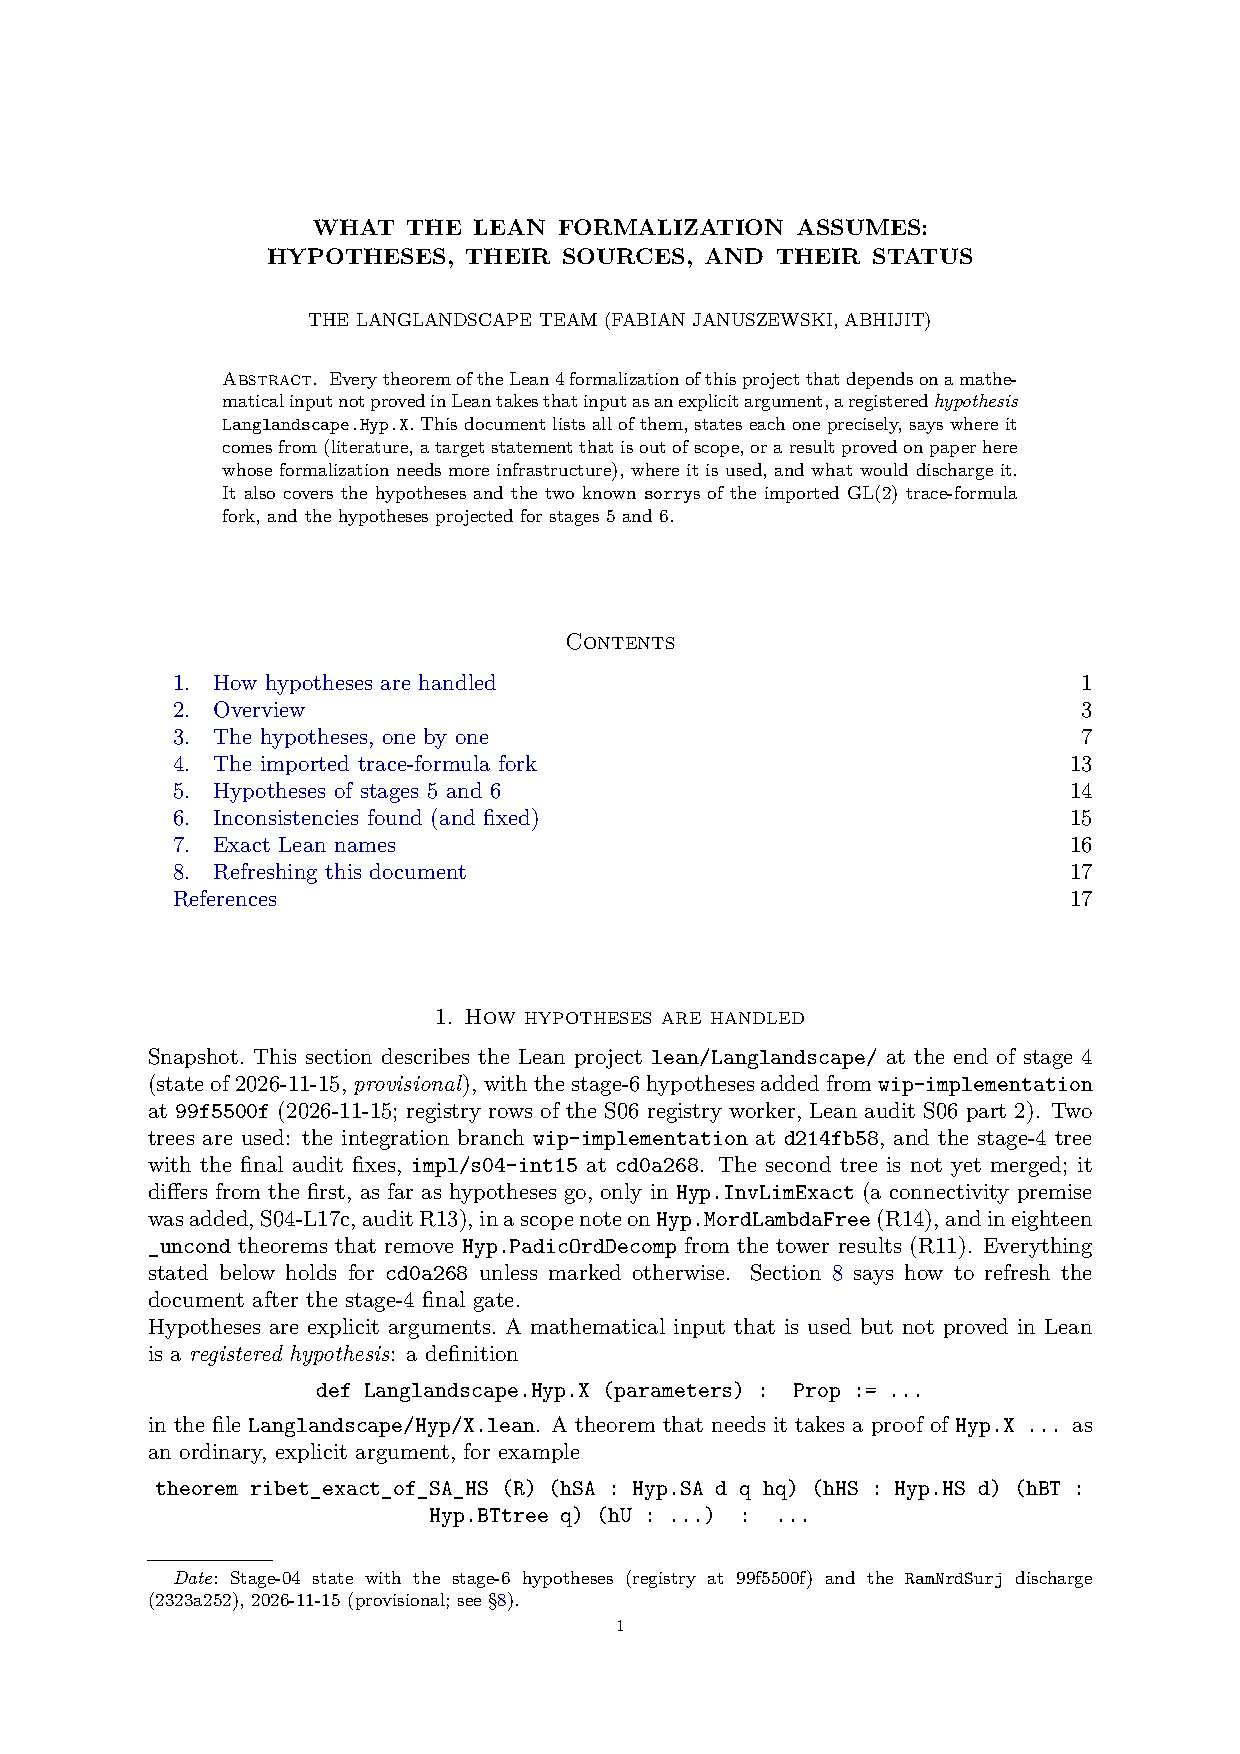
\includepdf[pages=-,scale=0.9,frame,pagecommand={\thispagestyle{plain}}]{../report/standalone-hypotheses.pdf}

\end{document}
